\documentclass[11pt,a4paper]{article}

\usepackage[utf8]{inputenc}
\usepackage[T1]{fontenc}
\usepackage{lmodern}
\usepackage[margin=1in]{geometry}
\usepackage{microtype}
\emergencystretch=3em % absorb small residual prose overfull boxes (inline math at line ends)
\usepackage{amsmath,amssymb,mathtools,amsthm}
\usepackage{booktabs}
\usepackage{enumitem}
\usepackage{graphicx}
\usepackage{placeins}
\usepackage{hyperref}

\graphicspath{{images_final/}}

\hypersetup{
    colorlinks=true,
    linkcolor=black,
    citecolor=black,
    urlcolor=blue
}

\newcommand{\E}{\mathbb{E}}
\newcommand{\Prob}{\mathbb{P}}
\newcommand{\R}{\mathbb{R}}
\newcommand{\Z}{\mathbb{Z}}
\newcommand{\Qcal}{\mathcal{Q}}
\newcommand{\Lcal}{\mathcal{L}}
\newcommand{\Acal}{\mathcal{A}}
\newcommand{\Fcal}{\mathcal{F}}
\newcommand{\dd}{\,\mathrm{d}}
\newcommand{\e}{\mathrm e}
\newcommand{\alphabar}{\bar\alpha}
\newcommand{\PnL}{\mathrm{PnL}}

\theoremstyle{plain}
\newtheorem{proposition}{Proposition}[section]
\newtheorem{approximation}[proposition]{Approximation}
\theoremstyle{definition}
\newtheorem{definition}{Definition}[section]
\newtheorem{remark}{Remark}[section]

% Float placement: allow denser pages so figure-heavy sections do not generate
% near-empty text pages.
\renewcommand{\topfraction}{0.9}
\renewcommand{\bottomfraction}{0.8}
\renewcommand{\textfraction}{0.07}
\renewcommand{\floatpagefraction}{0.75}
\setcounter{topnumber}{3}
\setcounter{bottomnumber}{2}
\setcounter{totalnumber}{4}

\title{Market Making with Persistent Flow Imbalance and Alpha}
\newcommand\blfootnote[1]{%
  \begingroup
  \renewcommand\thefootnote{}\footnote{#1}%
  \addtocounter{footnote}{-1}%
  \endgroup
}
\author{%
  Felipe Moret \quad Fabrizio Lillo \\[2pt]
  \small Scuola Normale Superiore di Pisa \\
  \small \texttt{felipebueno.moret@sns.it}, \;
  \texttt{fabrizio.lillo@sns.it}%
}
\date{}

\begin{document}

\maketitle
\blfootnote{Code, data, and paper source are available at
\url{https://github.com/felipemoret77/flow-imbalance-market-making}.}

\begin{abstract}
Classical market-making models in the Avellaneda--Stoikov and
Gu\'eant--Lehalle--Fernandez-Tapia (GLFT) tradition assume that buy and sell
market orders arrive at constant, symmetric rates.  Empirically, trade signs
are persistent and order-flow imbalance is informative about short-horizon
price changes.  We study how a market maker can adapt when this directional
pressure also evolves across slow regimes.  A market maker that keeps quoting
symmetrically under persistent one-sided flow accumulates inventory on the
losing side and, when flow predicts returns, is adversely selected.
This paper adapts the constant-absolute-risk-aversion (CARA) market-making
benchmark to persistent order flow through a sequence of increasingly
realistic models.  The first adds a persistent order-flow imbalance that shifts
the composition of buy and sell trades; the second lets that imbalance
generate a short-lived price drift; the third adds a slowly switching regime
that distinguishes transient imbalance from persistent flow pressure.  Each
model preserves the tractable inventory structure of the GLFT benchmark and
yields interpretable closed-form quoting approximations that skew the benchmark
quotes in response to observed flow.  Around the baseline calibrations,
common-path simulations show that the resulting policies markedly reduce the
adverse selection---or, in the martingale toy model, the flow-induced inventory
accumulation---suffered by the signal-blind benchmark, control inventory more
tightly, and improve the reported running-penalty performance diagnostic in the
alpha and regime-switching environments.  The stationary formulas are
conditional on the assumed large-horizon stabilization of the reduced HJB.
\end{abstract}

\section{Introduction}
\label{sec:intro}

A market maker (MM) in a limit order book (LOB) continuously posts bid and
ask quotes around a reference price, earning the quoted spread on round-trip
fills while carrying the inventory risk of the directional position
accumulated from asymmetric execution between them.  The canonical analytical
treatment frames this as a stochastic-control problem: the MM chooses signed
quote distances, the market responds with random market-order (MO) arrivals,
and the agent trades spread capture against the variance of marked-to-market
wealth.  The inventory-control view of the dealer's problem goes back to Ho and
Stoll~\cite{HoStoll1981}; its modern continuous-time formulations, the
closed-form benchmarks of Avellaneda and
Stoikov~\cite{AvellanedaStoikov2008} and of Gu\'eant, Lehalle, and
Fernandez-Tapia (GLFT)~\cite{GLFT2013}, are the reference points of this
literature (see \cite{Gueant2016} for a book-length treatment).
Both adopt a constant-absolute-risk-aversion (CARA) objective
and three stylized assumptions: a diffusive reference price, a fill intensity
that decays exponentially in quote distance, and \emph{constant, symmetric}
buy- and sell-side MO arrival rates.  Under these assumptions the stationary
quoting rule is, in the large-inventory limit, a half-spread that does not
depend on inventory plus a skew proportional to the inventory held: the
benchmark maker leans against its own position and against nothing else, since
the buy/sell composition of incoming market orders never enters its quotes.

\paragraph{Why the benchmark must be adapted.}
The constant-symmetric-rate assumption is counterfactual at microstructure
timescales: trade signs exhibit long
memory~\cite{LilloFarmer2004,BouchaudGefenPottersWyart2004}, a stylized fact
surveyed together with its price-impact counterpart
in~\cite{BouchaudFarmerLillo2008}, while order-flow imbalance explains
short-horizon price changes~\cite{ContKukanovStoikov2014} and is itself a
usable predictor of the future mid-price~\cite{Stoikov2018}.  This persistence
is not a primitive of the flow but the footprint of an execution mechanism:
large institutional orders---\emph{meta-orders}---are worked incrementally as
long sequences of child orders, so that a heavy-tailed distribution of parent
sizes produces a slowly decaying autocorrelation of executed
signs~\cite{LilloMikeFarmer2005}, and on horizons shorter than a few hours the
measured autocorrelation is attributable to this splitting by single investors
rather than to herding across them~\cite{TothPalitLilloFarmer2015}.  These
observations motivate a state-dependent model.  They also motivate, as a
further extension, a slowly switching directional-pressure state: meta-orders
have a finite execution phase followed by a distinct post-execution
phase~\cite{BacryIugaLasnierLehalle2015}, and the persistence of order flow is
itself regime-structured, with change points detectable online from public
flow~\cite{TsaknakiLilloMazzarisi2025}.  We do not identify the regime of
Section~\ref{sec:regime} with any individual meta-order---the observed
imbalance aggregates many concurrent executions, and a chain with exponential
dwell times is a one-timescale reduction of a broadly dispersed duration
distribution; the meta-order is the economic referent that makes a slowly
switching imbalance level the natural state variable, not a literal
description of it.  A maker quoting symmetrically under persistent
one-sided flow accumulates inventory; when that flow predicts subsequent price
changes, the inventory sits on the losing side and the maker is adversely
selected---the inventory-risk counterpart, in a quoting model, of the
information-based spread of Glosten and Milgrom~\cite{GlostenMilgrom1985}.  A
constant-rate benchmark cannot see this failure, which is documented for fast
liquidity providers, who absorb the early child orders of an institutional
meta-order into the opposite position~\cite{vanKervelMenkveld2019}.  We keep
the tractable CARA structure of GLFT but let the order-flow process drive the
quotes, through a sequence of increasingly state-dependent models.

\paragraph{Contributions.}
\begin{itemize}[leftmargin=1.2em,itemsep=1pt,topsep=2pt]
\item \textbf{Flow-imbalance toy model.}  We introduce an Ornstein--Uhlenbeck
  imbalance state \(I_t\) whose slow mean reversion makes the order-flow
  imbalance persistent; it reweights the composition of buy and sell MO flow while
  keeping the reference price a martingale, so that the only new channel is
  execution asymmetry.  We derive the corresponding Hamilton--Jacobi--Bellman
  (HJB) equation and its \emph{reduced} form---the equation for the inventory
  value alone, obtained by factoring out cash and reference price through CARA
  translation invariance---together with a closed-form ``tilted-GLFT'' ansatz---an odd imbalance
  loading, a flow-dependent inventory curvature, and a side-asymmetric cubic
  term---with no fitted constants.
\item \textbf{Fast-alpha model.}  We let aggregate directional flow generate
  a short-lived price drift (alpha).  When alpha mean-reverts much faster
  than the imbalance, a separation of time scales replaces it by its
  leading-order (frozen-\(i\)) conditional mean \(\alphabar(i)\), which enters
  the reduced HJB through the inventory-weighted drift reward
  \(q\alphabar(i)\).
\item \textbf{Slow-regime model.}  We add a slow Markov regime that shifts
  the mean-reversion level of the imbalance process, letting the policy
  distinguish transient imbalance from persistent flow pressure.
\item \textbf{A unifying optimal-quote map and closed-form approximations.}  All three
  models share the same CARA optimal-quote map---the optimal bid and ask
  depths are read off adjacent inventory differences of a reduced value
  function---and differ only in what drives that reduced value: a finite
  principal eigenvector in the signal-blind case and an ergodic reduced-HJB
  (RHJB) solution otherwise, conditional on the large-horizon stabilization
  of Remark~\ref{rem:ergodic_existence}.  In each case we obtain a closed-form ansatz by
  modulating the GLFT inventory curvature with the flow state and adding
  interpretable saturating signal loadings.
\item \textbf{Common-path evaluation.}  We compare the signal-blind GLFT
  benchmark against the state-dependent policies on matched realizations of a
  full jump-diffusion simulator, at a deliberately strong-signal calibration.
  In the regime environment the penalized-PnL ladder rises by \(+4435\)
  (paired s.e.\ \(5.2\)) when flow composition is observed and \(+1967\)
  (\(4.2\)) when alpha is used; the perfectly observed regime adds a further
  \(+175\) (\(1.8\)), which we do not read as the pure value of regime
  information (Section~\ref{sec:regime}).  In the fast-alpha environment the
  hybrid closed form is statistically indistinguishable from its RHJB
  (\(-0.8\pm1.1\)).  The first step is partly attributable to the benchmark's
  own risk calibration rather than to flow information
  (Remark~\ref{rem:blind_recalibration}).
\end{itemize}

\paragraph{Related work.}
The CARA market-making problem originates with Avellaneda and
Stoikov~\cite{AvellanedaStoikov2008}; its large-horizon, finite-inventory
analysis and the resulting closed-form quoting rule are due to Gu\'eant,
Lehalle, and Fernandez-Tapia~\cite{GLFT2013}.  Gu\'eant~\cite{Gueant2017}
shows that the CARA terminal-utility model used here and the
running-inventory-penalty model of Cartea, Jaimungal, and
Penalva~\cite{CarteaJaimungalPenalva2015} are two members of one family of
reduced HJBs with running inventory term \(\phi q^2\),
\(\phi=\tfrac12\gamma\sigma^2\) under CARA.  We derive the policies under the
CARA objective---exactly for the GLFT benchmark, up to the signal-risk-neutral
simplification of Definition~\ref{def:srn_rhjb} for the state-dependent
ones---and score them with the running-penalty diagnostic
(Remark~\ref{rem:xi}).  The exponential fill law we retain is one member of
the general intensity families analysed by Gu\'eant and
Lehalle~\cite{GueantLehalle2015}.  Approximating the reduced value by a
polynomial in inventory, substituting it into the reduced HJB and matching
powers of \(q\) to obtain elementary quotes is the device of
Gu\'eant~\cite{Gueant2017} and of Bergault, Evangelista, Gu\'eant, and
Vieira~\cite{BergaultEvangelistaGueantVieira2021}; what is new here is that the
matched coefficients carry a flow-dependent curvature rather than constants.

Signal-aware market making is the branch closest to this paper.  Cartea,
Jaimungal, and Ricci~\cite{CarteaJaimungalRicci2014} let a short-term
alpha and order-flow information enter the maker's quotes; Cartea and
Jaimungal~\cite{CarteaJaimungal2015} study the resulting risk profile, and
Cartea, Donnelly, and Jaimungal~\cite{CarteaDonnellyJaimungal2018} let a
finite-state Markov chain of volume imbalance modulate both the buy/sell
market-order intensities and the direction of mid-price jumps, solving the
resulting market-making problem numerically---the closest model to ours in
structure.  Closest in mechanism is Cartea and
Wang~\cite{CarteaWang2020}, where the alpha itself is generated by the
execution of liquidity-taking orders, as in Section~\ref{sec:fast_alpha}.
Order-book imbalance as the state that drives both the fill probability and the
adverse selection of a resting order is studied by Lehalle and
Mounjid~\cite{LehalleMounjid2017}, and a persistent, mean-reverting
price-direction state drives the market maker of Fodra and
Pham~\cite{FodraPham2015}.  The companion execution
problem with an order-flow state is treated in~\cite{CarteaJaimungal2016}.
Those models let the signal enter the price drift; in
\cite{CarteaJaimungalRicci2014} the market-order arrivals are themselves
modulated by a self- and mutually exciting process, so clustered one-sided
flow is present there too, and the quotes are obtained numerically.  Our
order-flow state differs in what makes closed forms possible: a single
one-dimensional OU imbalance drives both the buy/sell composition of fills and
the alpha, preserves the Cole--Hopf structure of the GLFT inventory block at
fixed imbalance, and yields a skew that can be written in elementary form.
The channel we isolate first is execution asymmetry alone: in the toy model of
Section~\ref{sec:toy} the price is a martingale and the flow state acts
\emph{only} through the composition of buy and sell fills, so the skew is pure
execution asymmetry rather than drift chasing; alpha is then added on top in
Section~\ref{sec:fast_alpha}.  Regime-switching microstructure states have
been used in high-frequency control by Guilbaud and
Pham~\cite{GuilbaudPham2013}, where a Markov chain drives the spread; in
Section~\ref{sec:regime} the chain instead shifts the mean-reversion level of
the imbalance itself, so the regime is informative about the \emph{future}
path of the flow rather than about current quoting costs.

\section{Probabilistic Setup and Signed Depths}
\label{sec:setup}

We write RHJB for ``reduced HJB'' throughout.
We work on a filtered probability space
\[
(\Omega,\Fcal,(\Fcal_t)_{t\ge0},\Prob)
\]
satisfying the usual conditions.  We take \((\Fcal_t)\) to be the usual
augmentation of the filtration generated jointly by the driving Brownian
motions, independent Poisson random measures on \(\R_+\times\R_+\), each with
intensity \(\dd t\,\dd z\), the initial state, and---in the regime
extension---the regime chain.  The point-process primitives include
\(\Pi^{N,a},\Pi^{N,b}\) for maker fills and, when aggregate flow is introduced
in the fast-alpha model, \(\Pi^{M,a},\Pi^{M,b}\).  These primitive sources are
mutually independent unless stated otherwise.  In particular, the controlled fill
processes are outputs of the model rather than generators of the filtration.
All state processes are adapted to \((\Fcal_t)\), and quote controls are
\((\Fcal_t)\)-predictable signed-depth processes.
At the baseline level the controlled state is cash, reference price, and
inventory:
\[
X_t\in\R,\qquad S_t\in\R,\qquad Q_t\in\Z.
\]
The state is enlarged only when a new economic channel is introduced: the toy
model adds \(I_t\), the fast-alpha simulation adds \(\alpha_t\), and the
regime extension adds \(R_t\).  Lower-case variables such as \(q,i,\alpha,r\)
are state values used in equations (the side index \(a\) of \(\delta^a\) below
is unrelated); upper-case variables such as
\(Q_t,I_t,\alpha_t,R_t\) denote the corresponding stochastic processes in the
original model, the process/value distinction for alpha being carried by the
time subscript.

Unless explicitly stated otherwise, the price, imbalance, and alpha noises
\(W^S\), \(W^I\), and \(W^\alpha\) are independent standard
\((\Fcal_t)\)-Brownian motions.  This convention removes mixed second-order
terms from the HJBs.

The market maker posts an ask quote and a bid quote around the reference price
\(S_t\):
\[
S_t^a=S_t+\delta_t^a,\qquad S_t^b=S_t-\delta_t^b.
\]
Thus
\[
\delta_t^a=S_t^a-S_t,\qquad \delta_t^b=S_t-S_t^b.
\]
Following the ask/bid convention of \cite{GLFT2013,Gueant2017}, we write
\(\delta^a\) for the ask depth and \(\delta^b\) for the bid depth; when a
statement applies to both sides we use the side index \(\ell\in\{a,b\}\).  The
depths \(\delta^a\) and \(\delta^b\) are signed distances to the reference
price.  A positive depth is away from the reference price; a negative depth is
price-improving relative to the reference.  The fill intensities of the market
maker's counting processes \(N^\ell\) are reduced-form exponential functions of
these signed depths:
\begin{equation}
\lambda_t^a
=\Lambda_t^{a,0}\e^{-k\delta_t^a},
\qquad
\lambda_t^b
=\Lambda_t^{b,0}\e^{-k\delta_t^b},
\label{eq:generic_fill_intensities}
\end{equation}
where \(k>0\) is the depth-decay parameter.  The zero-depth intensities
\(\Lambda_t^{a,0}\) and \(\Lambda_t^{b,0}\) are exogenous, nonnegative, and
uniformly bounded---there is \(\Lambda_{\max}<\infty\) with
\(\Lambda_t^{\ell,0}\le\Lambda_{\max}\) for all \(t\), \(\Prob\)-a.s.\ (in
every model below \(\Lambda^{\ell,0}\le2\bar\Lambda\)); when they depend on a
state \(I_t\) we write \(\Lambda^{\ell,0}(i)\), so that
\(\Lambda_t^{\ell,0}=\Lambda^{\ell,0}(I_t)\).  The side \(a\)
refers to buy market orders hitting the market maker's ask; the side \(b\)
refers to sell market orders hitting the market maker's bid.  For an admissible
strategy \(\delta\), define the controlled fill processes pathwise by thinning
the primitive Poisson random measures,
\begin{equation}
N_t^{\ell,\delta}
=\int_{(0,t]}\!\int_{\R_+}
\mathbf 1_{\{z\le \lambda_s^\ell(\delta)\}}\,\Pi^{N,\ell}(\dd s,\dd z),
\qquad \ell\in\{a,b\}.
\label{eq:fill_thinning}
\end{equation}
We suppress the superscript \(\delta\) when the control is clear.  Then
\(N^\ell_t-\int_0^t\lambda_s^\ell\,\dd s\) is an
\((\Fcal_t)\)-martingale~\cite{Bremaud1981}; independence of \(\Pi^{N,a}\) and
\(\Pi^{N,b}\) makes the two sides fire at distinct instants almost surely, with
conditionally independent innovations given \(\Fcal_{t-}\) (Cox processes when
quotes do not feed back on fills; under feedback, \eqref{eq:fill_thinning} is
the appropriate construction).  Two consequences are used throughout: fills
move inventory one unit at a time, so the \(\pm1\) dynamics of
\eqref{eq:cash_inventory} are well posed, and the two channels enter
additively, so the dynamic-programming equation is optimized one side at a
time through the optimal-quote map of Section~\ref{subsec:quote_map}.

An ask fill decreases inventory by one.  A bid fill increases inventory by
one.  Cash and inventory therefore satisfy
\begin{equation}
\dd X_t=(S_t+\delta_t^a)\dd N_t^a
       -(S_t-\delta_t^b)\dd N_t^b,
\qquad
\dd Q_t=-\dd N_t^a+\dd N_t^b .
\label{eq:cash_inventory}
\end{equation}
The model bid-ask spread relative to the reference price is
\[
\delta_t^a + \delta_t^b .
\]
Inventory is restricted to a finite grid
\[
\Qcal=\{-q_{\max},\ldots,q_{\max}\}.
\]
Here \(q_{\max}\in\mathbb N\), \(q_{\max}\ge1\), is the largest absolute
inventory the market maker is willing
to carry. At the limit the maker withdraws the side whose fill would breach
it: holding \(q=q_{\max}\) it stops quoting the bid, and holding
\(q=-q_{\max}\) it stops quoting the ask, so a further outward fill cannot
occur and inventory never drifts past \(\pm q_{\max}\) (equivalently, the
breaching fill intensity is set to zero).  This
same finite set of inventory levels is also the state space on which the
numerical schemes operate.

The market maker has constant absolute risk aversion \(\gamma>0\) and
maximizes, over a fixed horizon \(T>0\), the expected exponential utility of
terminal marked-to-market wealth~\cite{AvellanedaStoikov2008}:
\begin{equation}
H(t,x,s,q)
=
\sup_{\delta^a,\delta^b}
\E_{t,x,s,q}
\left[-\exp\{-\gamma(X_T+Q_TS_T)\}\right],
\qquad
H(T,x,s,q)=-\exp\{-\gamma(x+qs)\},
\label{eq:as_objective}
\end{equation}
where the supremum is over the admissible controls defined next.

For the control problem we fix the class of admissible quoting strategies on
the filtered space \((\Omega,\Fcal,(\Fcal_t)_{t\ge0},\Prob)\) introduced above.

\begin{definition}[Admissible quoting strategies]
\label{def:admissible}
A quoting strategy is a pair \(\delta=(\delta^a,\delta^b)\) of real-valued
processes on \([0,T]\).  It is \emph{admissible}, written \(\delta\in\Acal\), if
\begin{enumerate}[leftmargin=2.4em,itemsep=1pt,topsep=2pt,label=\textup{(A\arabic*)}]
\item \(\delta^a\) and \(\delta^b\) are \((\Fcal_t)\)-predictable;
\item there is a constant \(\underline\delta\in\R\) with
  \(\delta_t^\ell\ge\underline\delta\) for all \(t\in[0,T]\), \(\Prob\)-almost
  surely; together with the standing bound
  \(\Lambda_t^{\ell,0}\le\Lambda_{\max}\), this makes the induced fill
  intensities \(\lambda_t^\ell=\Lambda_t^{\ell,0}\e^{-k\delta_t^\ell}\) of
  \eqref{eq:generic_fill_intensities} uniformly bounded,
  \(\lambda_t^\ell\le\Lambda_{\max}\e^{-k\underline\delta}\);
\item \(\E\!\int_0^T\bigl(\lambda_t^a+\lambda_t^b\bigr)\,\dd t<\infty\).
\end{enumerate}
\end{definition}

Predictability in \textup{(A1)} means that the quotes posted over an
infinitesimal interval use only information strictly prior to it, so the
controlled counting processes \(N^\ell\) are well-defined point processes with
predictable intensities~\cite{Bremaud1981}; the lower bound \textup{(A2)} and the integrability
\textup{(A3)} rule out arbitrarily aggressive price-improving quotes and
explosive fill rates.  Under \textup{(A1)}--\textup{(A3)}, and on the finite
inventory grid \(\Qcal\), the controlled state \((X_t,S_t,Q_t)\) together with
any exogenous state is a bounded-rate jump--diffusion semimartingale adapted to
\((\Fcal_t)\), Markov under Markovian feedback quoting: it admits a unique non-explosive solution, and the expected
terminal utility in \eqref{eq:as_objective} is finite.

\begin{remark}[Reference price and market microstructure]
The reference price \(S_t\) may be read as a mid-price, but the model does
not represent the displayed best bid and ask: negative signed depths are
price-improving quotes relative to \(S_t\), to be viewed as marketable orders
if they would cross the opposite best quote.  This abstraction keeps the
smooth exponential law \eqref{eq:generic_fill_intensities}.
\end{remark}

\subsection{The CARA optimal-quote map}
\label{subsec:quote_map}

Every control problem in this paper is of the same type as
\eqref{eq:as_objective}: a CARA maker maximizing expected exponential utility
of terminal marked-to-market wealth over the admissible class \(\Acal\), on
the finite inventory grid \(\Qcal\), with a well-posed exogenous state (a
joint Markov switching diffusion, with pure-chain and pure-diffusion cases
included; see
Proposition~\ref{prop:verification}).  This subsection records the quoting
machinery---margin, curvature, and optimal-quote map---shared by every model.

\paragraph{GLFT scale constants.}
Two constants recur throughout: the inventory-independent execution margin
\(\delta_\gamma\) produced by the one-sided CARA quote optimization, and the
optimized-execution multiplier \(\chi_\gamma\),
\begin{equation}
\delta_\gamma
:=\frac1\gamma\log\left(1+\frac{\gamma}{k}\right),
\qquad
\chi_\gamma
:=\left(1+\frac{\gamma}{k}\right)^{-(1+k/\gamma)}.
\label{eq:delta_gamma}
\end{equation}

\paragraph{CARA optimal-quote map.}
The CARA objective is translation invariant in marked-to-market wealth, so in
every model the value factorizes as
\[
H=-\exp\{-\gamma(x+qs+u_q(z))\}
\]
for an exogenous state \(z\), where \(u_q(z)\) is the reduced 
value.  The optimal depths follow from a one-sided first-order condition.  An
ask fill takes \(q\to q-1\) and changes marked-to-market wealth by exactly
\(\delta^a\), so the post-/pre-fill value ratio is
\[
\frac{H(t,\,\cdot\,,q-1,z)}{H(t,\,\cdot\,,q,z)}
=\exp\bigl\{-\gamma\bigl(\delta^a+u_{q-1}(z)-u_q(z)\bigr)\bigr\},
\]
and the ask contribution to the dynamic-programming equation is proportional,
with the positive constant \(|H|\), to
\[
\Lambda^{a,0}\,\e^{-k\delta^a}
\Bigl[1-\exp\bigl\{-\gamma\bigl(\delta^a+u_{q-1}(z)-u_q(z)\bigr)\bigr\}\Bigr].
\]
The zero-depth intensity \(\Lambda^{a,0}\) scales the bracket but does not
enter the optimization; maximizing over \(\delta^a\) gives the first-order
condition
\[
\exp\bigl\{-\gamma\bigl(\delta^{a,\star}+u_{q-1}(z)-u_q(z)\bigr)\bigr\}
=\Bigl(1+\tfrac{\gamma}{k}\Bigr)^{-1},
\]
that is, \(\delta^{a,\star}=\delta_\gamma+u_q(z)-u_{q-1}(z)\) with the margin
\(\delta_\gamma\) of \eqref{eq:delta_gamma}; the bid side is identical with
\(q+1\) in place of \(q-1\).  The optimal-quote map is therefore the margin
plus an adjacent inventory difference of the reduced value,
\begin{equation}
\delta^a(q,z)=\delta_\gamma+u_q(z)-u_{q-1}(z)\quad(q\neq-q_{\max}),
\qquad
\delta^b(q,z)=\delta_\gamma+u_q(z)-u_{q+1}(z)\quad(q\neq q_{\max}).
\label{eq:state_dep_recovery}
\end{equation}
Equation~\eqref{eq:state_dep_recovery} is the CARA optimal-quote map used by
every model in this paper~\cite{AvellanedaStoikov2008,GLFT2013}; at inventory
boundaries the unavailable neighbor is dropped---no bid at \(q=q_{\max}\), no
ask at \(q=-q_{\max}\).

\subsection{The GLFT benchmark}
\label{subsec:glft}

The signal-blind GLFT benchmark~\cite{AvellanedaStoikov2008,GLFT2013} is the
special case in which the reference price is a martingale,
\(\dd S_t=\sigma\,\dd W^S_t\), and the two zero-depth MO intensities are
constant and symmetric,
\(\Lambda^{a,0}=\Lambda^{b,0}=\bar\Lambda>0\).  It is the
inventory-only baseline that the rest of the paper modulates with order-flow
information.

\paragraph{Exact finite-grid benchmark.}
Through the optimal-quote map \eqref{eq:state_dep_recovery}, the signal-blind
reduced value is \(u_q=\tfrac1k\log\theta_q\), where the Cole--Hopf profile
\(\theta(\tau)\) (with \(\tau=T-t\) and \(\theta(0)=\mathbf 1\)) solves the
linear system \(\partial_\tau\theta=\mathsf A_{\rm GLFT}\theta\)
on \(\Qcal\), with the tridiagonal inventory operator
\[
(\mathsf A_{\rm GLFT})_{q,q'}=
\begin{cases}
-d_q, & q'=q,\\
c_{\rm GLFT}, & q'=q\pm1\in\Qcal,\\
0, & \text{otherwise},
\end{cases}
\qquad
d_q=a_{\rm c}q^2,
\quad
a_{\rm c}=\tfrac{k}{2}\gamma\sigma^2,
\quad
c_{\rm GLFT}=\bar\Lambda\chi_\gamma .
\]
\begin{proposition}[Finite-grid stationary GLFT benchmark]
\label{prop:glft_stationary}
The matrix \(\mathsf A_{\rm GLFT}\) has a largest eigenvalue
\(\lambda_{\rm GLFT}\) that is \emph{simple}---an unrepeated root, so its
eigenspace is one-dimensional and the eigenvector is unique up to
scaling---with a strictly positive eigenvector
\(f=(f_q)_{q\in\Qcal}\) solving \(\mathsf A_{\rm GLFT}f=\lambda_{\rm GLFT}f\),
\(f_q>0\).  For the finite-horizon solution
\(\theta(\tau)=\exp\{\tau\mathsf A_{\rm GLFT}\}\mathbf 1\), the neighboring
component ratios \(\theta_q/\theta_{q\pm1}\) converge as \(\tau\to\infty\) to
the eigenvector ratios \(f_q/f_{q\pm1}\) (the scaling cancels), so the
stationary finite-grid GLFT depths are
\begin{equation}
\delta_{\rm GLFT}^{a,\infty}(q)
=\delta_\gamma+\frac1k\log\frac{f_q}{f_{q-1}},
\quad q>-q_{\max},\qquad
\delta_{\rm GLFT}^{b,\infty}(q)
=\delta_\gamma+\frac1k\log\frac{f_q}{f_{q+1}},
\quad q<q_{\max}.
\label{eq:glft_stationary_depths}
\end{equation}
\end{proposition}
The Perron--Frobenius argument is given in \cite{GLFT2013}; this finite-grid
eigenvector is the exact stationary GLFT reference.  The Monte Carlo comparisons
simulate its Gaussian continuum limit
\eqref{eq:glft_closed_ask}--\eqref{eq:glft_closed_bid} below.

\paragraph{Closed-form (Gaussian) quotes.}
On a wide grid the eigenvector \(f\) varies slowly between adjacent inventory
levels, so the inventory index can be treated as a continuous variable and
\(f\) is well approximated by a Gaussian, \(f_q\approx C\e^{-r_{\rm G}q^2/2}\)
(derived in \cite{GLFT2013}), with decay rate---whence the subscript
\(\mathrm G\)---
\[
r_{\rm G}=\sqrt{\frac{a_{\rm c}}{c_{\rm GLFT}}}.
\]
Substituting this profile in \eqref{eq:glft_stationary_depths} makes the depths
affine in inventory; this is the large-inventory continuum limit, which we mark
with a superscript \(\mathrm G\) (Gaussian),
\begin{align}
\delta_{\rm GLFT}^{a,\mathrm G}(q)
&=
\delta_\gamma-\frac{r_{\rm G}}{2k}\,(2q-1),
\label{eq:glft_closed_ask}\\
\delta_{\rm GLFT}^{b,\mathrm G}(q)
&=
\delta_\gamma+\frac{r_{\rm G}}{2k}\,(2q+1),
\label{eq:glft_closed_bid}
\end{align}
with \(\delta_\gamma,\chi_\gamma\) as in \eqref{eq:delta_gamma}.  Each term has
a direct reading.  The margin \(\delta_\gamma\) is the inventory-independent
transaction margin from the one-sided execution problem; it is \emph{not} the
full half-spread, because the inventory-risk curvature adds \(r_{\rm G}/(2k)\) to
both quotes, so the \(q\)-independent half-spread is
\[
\tfrac12\bigl(\delta_{\rm GLFT}^{a,\mathrm G}(q)+\delta_{\rm GLFT}^{b,\mathrm G}(q)\bigr)
=\delta_\gamma+\frac{r_{\rm G}}{2k}.
\]
The margin \(\delta_\gamma\) decreases in both \(\gamma\) and \(k\), with
risk-neutral limit \(1/k\) as \(\gamma\to0\) (the dimensionless margin
\(\gamma\delta_\gamma=\log(1+\gamma/k)\) increases in the risk-to-liquidity ratio
\(\gamma/k\)).  The linear term is the inventory skew: a maker holding
positive inventory lowers both quotes to revert toward a flat book, at a rate
set by the curvature \(r_{\rm G}\), which steepens with volatility and risk
aversion (larger \(a_{\rm c}\)) and flattens with liquidity (larger
\(c_{\rm GLFT}\)).  The two sides are skewed symmetrically precisely because
the flow is symmetric, \(\Lambda^{a,0}=\Lambda^{b,0}\).

\paragraph{Limitations.}
Under persistent, directional flow a maker quoting by
\eqref{eq:glft_closed_ask}--\eqref{eq:glft_closed_bid} keeps a symmetric skew,
accumulates inventory on the side being adversely filled, and cannot lean on a
drift it does not model.  The next three sections relax the constant-symmetric
flow and martingale-price assumptions one channel at a time---flow composition
(Section~\ref{sec:toy}), induced alpha (Section~\ref{sec:fast_alpha}), and a
slow regime (Section~\ref{sec:regime})---while keeping the same
\(\delta_\gamma\) margin, inventory curvature, and optimal-quote map.

% [Archived: the original commented-out GLFT section was moved to old_glft_derivations.tex (it was an inert \iffalse block; essentials are in the Introduction and Sec.~\ref{sec:setup}).]

\section{Flow-Imbalance Toy Model}
\label{sec:toy}

Throughout this section \(H(t,x,s,q,i)\) is the value function in the original
state variables and, as in Section~\ref{subsec:quote_map},
\(H=-\exp\{-\gamma(x+qs+u_q(t,i))\}\); the reduced HJB is the equation for
\(u_q(t,i)\) after this CARA wealth/price reduction.

\subsection{Primitive Imbalance State}

The first state-dependent extension we propose adds an
Ornstein--Uhlenbeck (OU) imbalance factor \(I_t\) with mean-reversion rate
\(\beta>0\) and volatility \(\eta>0\):
\begin{equation}
\dd I_t=-\beta I_t\,\dd t+\eta\,\dd W^I_t.
\label{eq:toy_ou}
\end{equation}
The reference price remains a martingale:
\[
\dd S_t=\sigma\,\dd W^S_t.
\]
Thus this model has flow imbalance but no alpha drift.
In this extension, the zero-depth buy and sell intensities are given by
\begin{align}
\Lambda^{a,0}(i)
&=\bar\Lambda(1+\tanh i)
=\bar\Lambda\frac{\e^i}{\cosh i},
\label{eq:lambda_plus_y}\\
\Lambda^{b,0}(i)
&=\bar\Lambda(1-\tanh i)
=\bar\Lambda\frac{\e^{-i}}{\cosh i}.
\label{eq:lambda_minus_y}
\end{align}
Therefore
\[
\Lambda^{a,0}(i)+\Lambda^{b,0}(i)=2\bar\Lambda,
\qquad
\frac{\Lambda^{a,0}(i)}{\Lambda^{b,0}(i)}=\e^{2i}.
\]
The state \(I_t\) reallocates activity between the ask and bid sides while
keeping total zero-depth activity constant.  Positive \(i\) means buy market
orders are more likely; negative \(i\) means sell market orders are more
likely.

Figure~\ref{fig:toy_intro_sample_path} illustrates this intensity structure.  At any imbalance level \(i\) the
zero-depth rates only reallocate a fixed total \(2\bar\Lambda\) between the two
sides, and each side then decays exponentially in the quoted depth,
\(\Lambda^\ell(i,\delta)=\Lambda^{\ell,0}(i)\,\e^{-k\delta}\).  The state
dependence is thus confined to the zero-depth level \(\Lambda^{\ell,0}(i)\);
the depth decay keeps the exponential shape that makes the CARA reduction
explicit, and which \cite{GueantLehalle2015} places within a broader family of
admissible intensity shapes.

\begin{figure}[htbp]
\centering
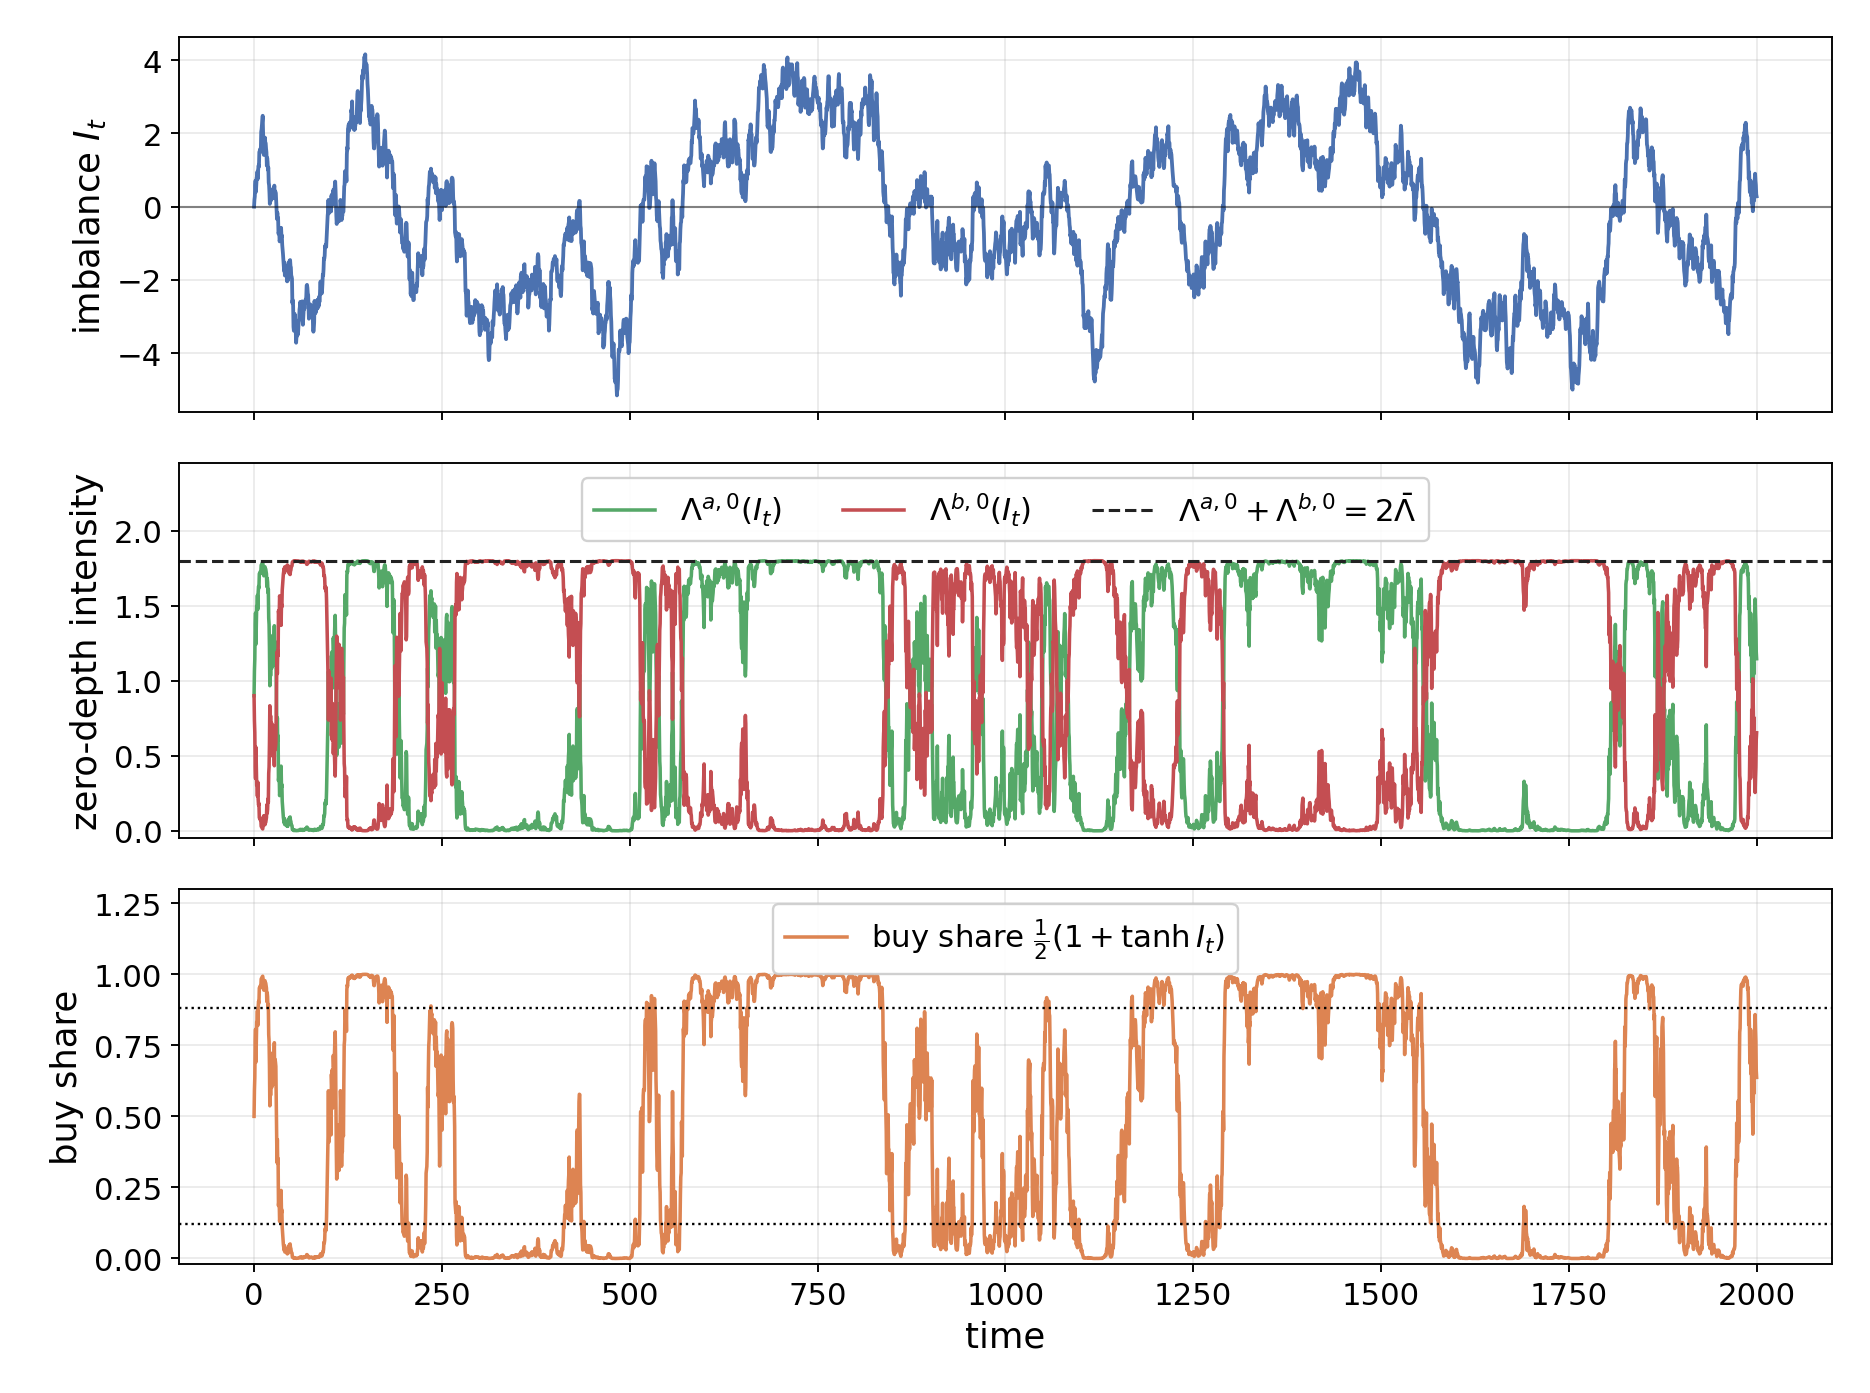
\includegraphics[width=0.8\linewidth]{toy_intro_ou_lambda_sample_path_v2.png}
\caption{Toy model: an OU imbalance path \(I_t\) (top); the induced
zero-depth side intensities \(\Lambda^{a,0}(I_t),\Lambda^{b,0}(I_t)\), whose sum
stays pinned at \(2\bar\Lambda\) (middle); and the buy share
\(\tfrac12(1+\tanh I_t)\) with the \(0.12\)--\(0.88\) band used in the
calibration discussion of Section~\ref{sec:toy} (bottom).  On this path the
share lies outside the band \(71\%\) of the time, against a stationary value of
about \(60\%\).}
\label{fig:toy_intro_sample_path}
\end{figure}


\FloatBarrier

\subsection{The HJB and Verification}

We first write the HJB in calendar time \(t\).  The terminal condition is
\[
H(T,x,s,q,i)=-\exp\{-\gamma(x+qs)\},
\qquad
u_q(T,i)=0.
\]
For interior inventory states, the dynamic programming equation in the
original variables is
\begin{align}
0={}&
\partial_t H(t,x,s,q,i)
+\frac{\sigma^2}{2}\partial_{ss} H(t,x,s,q,i)
+\Lcal_I H(t,x,s,q,i)
\notag\\
&+
\sup_{\delta^a\in\R}
\Lambda^{a,0}(i)\e^{-k\delta^a}
\Bigl[
H(t,x+s+\delta^a,s,q-1,i)-H(t,x,s,q,i)
\Bigr]
\notag\\
&+
\sup_{\delta^b\in\R}
\Lambda^{b,0}(i)\e^{-k\delta^b}
\Bigl[
H(t,x-s+\delta^b,s,q+1,i)-H(t,x,s,q,i)
\Bigr],
\label{eq:toy_full_hjb_t}
\end{align}
where the imbalance generator is
\[
\Lcal_I H
=-\beta i\,\partial_i H+\frac{\eta^2}{2}\partial_{ii} H
\]
when it acts on \(H\).  Relative to the signal-blind CARA--GLFT HJB, the
imbalance changes the equation in two ways: the new generator \(\Lcal_I H\)
is the only new continuous term (the price is still driftless, so its
contribution remains \(\sigma^2\partial_{ss}H/2\)), and the zero-depth fill
rates become \(\Lambda^{a,0}(i)\) and \(\Lambda^{b,0}(i)\), which rescales the
execution Hamiltonians without creating a new operator; the one-sided jump
structure and the two signed-depth controls are unchanged.

The dynamic programming equation \eqref{eq:toy_full_hjb_t} identifies the value
function by the following finite-grid verification of the \emph{exact} CARA
HJB, which applies here and, with the obvious changes, to the fast-alpha and
regime extensions below.

\begin{proposition}[Verification on the finite grid]
\label{prop:verification}
Fix the finite inventory grid \(\Qcal\).  Let the exogenous state
\(Z_t=(Y_t,R_t)\) be a Markov switching diffusion: conditional on the
finite-state chain \(R_t\), whose jump rates are bounded, the diffusion \(Y_t\)
has globally Lipschitz coefficients and at most linear growth.  A pure
diffusion (such as the OU imbalance \eqref{eq:toy_ou}) and a pure finite-state
chain are included as special cases.  Assume that the reference-price drift
and volatility used in the control problem are bounded functions of the
exogenous state.  Suppose \(H\) has the CARA form
\(H(t,x,s,q,z)=-\exp\{-\gamma(x+qs+u_q(t,z))\}\), with \(u\) bounded,
\(C^1\) in \(t\), and \(C^2\) in the diffusion coordinates for each regime.
Assume that \(\nabla_Yu_q\), the adjacent-inventory differences
\(u_q-u_{q\pm1}\), and regime-jump differences are bounded, that \(H\) solves
the joint switching jump--diffusion dynamic programming equation
\eqref{eq:toy_full_hjb_t}---or its fast-alpha and regime
analogues below---with the stated terminal condition, and that the per-side
supremum over the depth is attained by a measurable selector
\((\delta^{a,\star},\delta^{b,\star})\in\Acal\).  Then \(H\) equals the value
function of~\eqref{eq:as_objective} over \(\Acal\), and the selector is an
optimal Markov control.
\end{proposition}

\begin{proof}[Proof sketch]
Write \(\Xi_t=(X_t,S_t,Q_t,Z_t)\), \(g(\Xi_T):=-\e^{-\gamma(X_T+Q_TS_T)}\), and
\(\mathcal G^\delta\) for the generator of \(\Xi\) under the quoting control
\(\delta\).  On \(\Qcal\), \(\Xi\) is a jump--diffusion semimartingale with
bounded fill and switching rates (Markov under Markovian feedback quoting), so
for \(H\) of the assumed regularity the It\^o--Dynkin formula for switching
jump--diffusions~\cite{YinZhu2010} gives, for every \(\delta\in\Acal\) and \(t\le T\),
\begin{equation}
g(\Xi_T)=H(t,\Xi_t)
+\int_t^T\bigl(\partial_tH+\mathcal G^{\delta}H\bigr)(\rho,\Xi_\rho)\,\dd\rho
+M_T^\delta,
\label{eq:verif_dynkin}
\end{equation}
with \(M^\delta\) the local martingale of Brownian and compensated fill and
regime-jump integrals.  Put \(\mathcal W_t=X_t+Q_tS_t\).  Since
\(|Q_t|\le q_{\max}\) and the reference-price drift and volatility are bounded,
the continuous part of \(\mathcal W\) has finite exponential moments of every
order on \([0,T]\); fills change \(\mathcal W\) by
\(\delta_t^\ell\ge\underline\delta\) and, as
\(\lambda_t^\ell\le\Lambda_{\max}\e^{-k\underline\delta}\), their count is
dominated by a Poisson process of finite deterministic rate; hence
\(\sup_{t\le T}\E\exp\{-p\mathcal W_t\}<\infty\) for every \(p>0\).  The
switching diffusion \(Y\) (globally Lipschitz coefficients, at most linear
growth) has finite polynomial moments of every order
\cite{Pham2009,YinZhu2010}; its
diffusion matrix \(\Sigma_Y(z)\) need not be bounded, but bounded
\(\nabla_Yu_q\) gives
\(\lvert\Sigma_Y(z)^\top\nabla_Yu_q\rvert\le C(1+\lvert z\rvert)\), so Hölder's
inequality and these moments make the Brownian integrands square-integrable.
The fill- and regime-jump ratios are uniformly bounded (\(\delta^\ell\) bounded
below, adjacent-inventory and regime differences of \(u\) bounded, all rates
bounded).  Every component of \(M^\delta\) is thus square-integrable, so
\(M^\delta\) is a true martingale and \(\E_{t,x,s,q,z}[M_T^\delta]=0\).

Since \eqref{eq:toy_full_hjb_t} reads
\(\partial_tH+\sup_{\delta}\mathcal G^{\delta}H=0\), each side's execution
Hamiltonian being maximized pointwise at the selector, the integrand in
\eqref{eq:verif_dynkin} is nonpositive for every \(\delta\in\Acal\) and
vanishes identically under
\(\delta^\star:=(\delta^{a,\star},\delta^{b,\star})\).  Taking
\(\E_{t,x,s,q,z}\) in \eqref{eq:verif_dynkin} gives
\(H(t,x,s,q,z)\ge\sup_{\delta\in\Acal}\E_{t,x,s,q,z}[g(\Xi_T)]\), with equality
in the per-control bound at \(\delta^\star\in\Acal\), so that
\(H(t,x,s,q,z)=\E^{\,\delta^\star}_{t,x,s,q,z}[g(\Xi_T)]
\le\sup_{\delta\in\Acal}\E_{t,x,s,q,z}[g(\Xi_T)]\).  The two bounds combine,
so \(H\) is the value function of \eqref{eq:as_objective} and the measurable
selector \(\delta^\star\) attains the supremum: it is an optimal Markov
control.
\end{proof}

The two analogues invoked in the statement are obtained from
\eqref{eq:toy_full_hjb_t} without new operators: the fast-alpha problem of
Section~\ref{sec:fast_alpha} adds the drift term \(\alphabar(i)\,\partial_sH\),
which the CARA reduction turns into the reward \(q\alphabar(i)\) of
\eqref{eq:fast_alpha_hjb}, and the regime problem replaces \(\Lcal_I\) by the
joint generator \eqref{eq:regime_joint_generator}, which the reduction turns
into the block \eqref{eq:regime_cara_joint_cole_hopf}.

\subsection{CARA Reduction and the Reduced HJB}

Substituting the CARA form into \eqref{eq:toy_full_hjb_t} and dividing by
\(-\gamma H\) turns the imbalance generator into
\(\Lcal_IH/(-\gamma H)=\Lcal_Iu_q-\tfrac{\gamma\eta^2}{2}(\partial_i u_q)^2\).
The extra term \(-\tfrac{\gamma\eta^2}{2}(\partial_i u_q)^2\) is the
risk-sensitive CARA charge for signal uncertainty.  The imbalance diffusion
gives the continuation value instantaneous variance \(\eta^2(\partial_i u_q)^2\)
from the signal channel alone, and a CARA maker charges \(\tfrac\gamma2\) of this
variance---exactly as it charges \(\tfrac{\gamma\sigma^2}{2}q^2\) for inventory
(price) risk.

\begin{proposition}[Exact CARA reduction of the toy HJB]
\label{prop:toy_reduction}
With \(H=-\exp\{-\gamma(x+qs+u_q(t,i))\}\), the HJB \eqref{eq:toy_full_hjb_t} is
equivalent, in time-to-maturity \(\tau=T-t\), to
\begin{align}
\partial_\tau u_q
={}&
\Lcal_I u_q-\frac{\gamma\eta^2}{2}(\partial_i u_q)^2-\frac{\gamma\sigma^2}{2}q^2
\notag\\
&+\frac{\Lambda^{a,0}(i)}{k}\chi_\gamma\exp\{k(u_{q-1}-u_q)\}
+\frac{\Lambda^{b,0}(i)}{k}\chi_\gamma\exp\{k(u_{q+1}-u_q)\},
\label{eq:toy_exact_cara_hjb}
\end{align}
with optimal depths \(\delta^{a,\star}=\delta_\gamma+u_q-u_{q-1}\),
\(\delta^{b,\star}=\delta_\gamma+u_q-u_{q+1}\).
\end{proposition}

\begin{proof}
Dividing \eqref{eq:toy_full_hjb_t} by \(-\gamma H\) gives the OU term above and,
from the price term, \(\tfrac{(\sigma^2/2)\partial_{ss}H}{-\gamma H}=-\tfrac{\gamma\sigma^2}{2}q^2\).
Each one-sided optimization is that of Section~\ref{subsec:quote_map} with
\(z=i\), giving \(\delta^{\ell,\star}\) as stated and, on re-substitution, the
optimized execution rates
\(\tfrac{\Lambda^{\ell,0}(i)}{k}\chi_\gamma\e^{k(u_{q\mp1}-u_q)}\); passing to
\(\tau=T-t\) yields \eqref{eq:toy_exact_cara_hjb}.
\end{proof}

\begin{definition}[Signal-risk-neutral RHJB]
\label{def:srn_rhjb}
The \emph{signal-risk-neutral} reduced HJB drops the signal-risk term
\(-\tfrac{\gamma\eta^2}{2}(\partial_i u_q)^2\) from \eqref{eq:toy_exact_cara_hjb},
\begin{align}
\partial_\tau u_q
={}&
\Lcal_I u_q-\frac{\gamma\sigma^2}{2}q^2
+\frac{\Lambda^{a,0}(i)}{k}\chi_\gamma\exp\{k(u_{q-1}-u_q)\}
+\frac{\Lambda^{b,0}(i)}{k}\chi_\gamma\exp\{k(u_{q+1}-u_q)\},
\label{eq:toy_hjb}
\end{align}
with quotes given by the optimal-quote map \eqref{eq:state_dep_recovery}.
\end{definition}

Keeping this term would make the reduced HJB nonlinear in the signal direction;
we drop it, which keeps the OU propagation of \(I_t\) linear and preserves the
GLFT inventory structure.  The policy then still prices price and inventory risk
under CARA, but is risk-neutral with respect to signal uncertainty: it still
propagates the full future distribution of \(I_t\) through \(\Lcal_I\), yet does
not charge the CARA variance penalty \(\tfrac{\gamma\eta^2}{2}(\partial_i u_q)^2\)
for it.  The reduced policies are therefore optimal for \eqref{eq:toy_hjb} and
are signal-risk-neutral approximations to the exact CARA control of
Proposition~\ref{prop:verification}.

\subsection{Solving the Reduced HJB}

The reduced HJB \eqref{eq:toy_hjb} has two parts.  The inventory/fill part is
nonlinear in \(u\), but at fixed imbalance \(i\) the Cole--Hopf change
\(w=\e^{ku}\) makes it a linear tridiagonal operator on \(q\); the signal part
\(\Lcal_I\) is linear in \(u\) and acts along the imbalance grid at fixed
\(q\).  We therefore advance the equation by operator splitting---an inventory
sub-step in \(w\) alternating with a signal sub-step in \(u\), each an exact
matrix exponential---with the symmetric (Strang) ordering of
Section~\ref{subsec:strang}.

\subsubsection{Cole--Hopf Inventory Step}

At fixed \(i\), set
\[
w_q(\tau,i)=\e^{k u_q(\tau,i)}.
\]
The inventory part of \eqref{eq:toy_hjb} becomes
\begin{equation}
\partial_\tau w_q
=
-\frac{k}{2}\gamma\sigma^2q^2w_q
+
\chi_\gamma
\Lambda^{a,0}(i)w_{q-1}
+
\chi_\gamma
\Lambda^{b,0}(i)w_{q+1}.
\label{eq:toy_w}
\end{equation}
Thus, after the Cole--Hopf change, the inventory part is linear in
the vector
\[
w(i)=
\bigl(w_{-q_{\max}}(i),w_{-q_{\max}+1}(i),\ldots,w_{q_{\max}}(i)\bigr)^\top
\]
when \(i\) is held fixed.  With \(\chi_\gamma\) as in \eqref{eq:delta_gamma},
define
\[
c_+(i)=\chi_\gamma\Lambda^{a,0}(i),
\qquad
c_-(i)=\chi_\gamma\Lambda^{b,0}(i),
\qquad
d_q=\frac{k}{2}\gamma\sigma^2q^2 .
\]
At a fixed imbalance value \(i\), the inventory operator is
\[
(\mathsf A_i^{\rm toy}w)_q
=
-d_qw_q+c_+(i)w_{q-1}+c_-(i)w_{q+1},
\]
with the unavailable neighbor omitted at the inventory boundaries.  In the
ordered basis \((-q_{\max},\ldots,q_{\max})\) this is a tridiagonal matrix---a
single fill moves inventory only to \(q\pm1\)---whose upper and lower
off-diagonals differ unless \(\Lambda^{a,0}(i)=\Lambda^{b,0}(i)\), so the
fixed-\(i\) inventory matrix is generally non-symmetric.
Because this block is linear at fixed \(i\), the inventory sub-step over
\(\Delta\tau\) is the exact matrix exponential
\[
w(\tau+\Delta\tau,i)=\exp\{\Delta\tau\,\mathsf A_i^{\rm toy}\}\,w(\tau,i).
\]

Conditional on the current \(i\), this fixed-\(i\) inventory block keeps the same
tridiagonal GLFT structure as the signal-blind model; the coupling across
imbalance states is carried instead by the OU generator \(\Lcal_I\) in
\eqref{eq:toy_hjb}.

\subsubsection{Imbalance Signal Step}
\label{subsubsec:toy_signal_step}

The second piece of \eqref{eq:toy_hjb} is the propagation of the imbalance
state.  If the inventory part is suppressed, each inventory slice solves the
linear signal equation
\begin{equation}
\partial_\tau u_q(\tau,i)=\Lcal_Iu_q(\tau,i),
\qquad
\Lcal_I=-\beta i\,\partial_i+\frac{\eta^2}{2}\partial_{ii}.
\label{eq:toy_signal_step}
\end{equation}
This step has no quote optimization and no inventory jump; it only propagates
the continuation value under the mean reversion and diffusion of \(I_t\).
Discretize \(\Lcal_I\) by centered differences on the uniform \(I\)-grid
\(i_0<\cdots<i_{J-1}\) (spacing \(\Delta i\)), acting on the vector
\(U_q(\tau)=\bigl(u_q(\tau,i_0),\ldots,u_q(\tau,i_{J-1})\bigr)^\top\) at fixed
inventory \(q\).  With \(a_\Delta=\eta^2/(2\Delta i^2)\) and
\(b_j^\Delta=\beta i_j/(2\Delta i)\), the interior row \(0<j<J-1\) of the
resulting \(J\times J\) matrix \(\mathsf L_I^\Delta\) is
\[
(\mathsf L_I^\Delta U_q)_j
=(a_\Delta+b_j^\Delta)\,u_q(\tau,i_{j-1})
-2a_\Delta\,u_q(\tau,i_j)
+(a_\Delta-b_j^\Delta)\,u_q(\tau,i_{j+1}),
\]
so \(\mathsf L_I^\Delta\) is tridiagonal.  At the grid edges, where the centered
stencil would require off-grid nodes, we use instead a one-sided first
difference for the drift and a reflecting (Neumann) ghost-node closure
\(u_q(\tau,i_{-1})=u_q(\tau,i_1)\), \(u_q(\tau,i_J)=u_q(\tau,i_{J-2})\) for the
diffusion, so that the first row is
\((-2(a_\Delta-b_0^\Delta),\,2(a_\Delta-b_0^\Delta),\,0,\ldots,0)\) and the last
\((0,\ldots,0,\,2(a_\Delta+b_{J-1}^\Delta),\,-2(a_\Delta+b_{J-1}^\Delta))\).  Every row of
\(\mathsf L_I^\Delta\) sums to zero, and under the cell-P\'eclet condition
\(\beta\,i_{\max}\,\Delta i\le\eta^2\) of
Proposition~\ref{prop:finite_horizon} (satisfied here with ample margin) the
off-diagonal entries are nonnegative---unconditionally so in the boundary
rows, where the mean-reverting drift points into the grid---so
\(\mathsf L_I^\Delta\) is the
generator of a Markov chain reflected at the grid boundary.

Over a time increment \(\Delta\tau\), the signal
update is the matrix exponential
\[
U_q(\tau+\Delta\tau)
=
\exp\{\Delta\tau\,\mathsf L_I^\Delta\}\,U_q(\tau),
\]
applied separately for each inventory level \(q\).


\subsubsection{Strang Splitting}
\label{subsec:strang}

We therefore use a symmetric
half-step/full-step/half-step update:
\[
\partial_\tau u_q
=
\Lcal_Iu_q+\mathcal H_q(u;i),
\]
where \(\mathcal H_q(u;i)\) denotes the inventory-risk and optimized-fill
terms in \eqref{eq:toy_hjb}.  The word ``symmetric'' means that each time
step first moves \(I\) for half a time step, then updates inventory for a full
time step, and finally moves \(I\) for another half time step.

Concretely, each \(I\)-half-step is the matrix exponential
\(\exp\{\tfrac{\Delta\tau}{2}\mathsf L_I^\Delta\}\) applied to every inventory
slice \(U_q\) in the reduced value \(u\), and the middle
inventory step applies \(\exp\{\Delta\tau\,\mathsf A_{i_j}^{\rm toy}\}\) of
\eqref{eq:toy_w} to \(w=\e^{ku}\) at each fixed \(i_j\).  

\subsection{Ergodic and Spectral Interpretation}

Equation~\eqref{eq:toy_hjb} is autonomous in \(\tau\), suggesting a
large-horizon split into linear growth plus a stationary relative shape; this
stabilization is exact for the linear GLFT benchmark and an explicit
assumption for the nonlinear RHJB, not a consequence of autonomy alone.  In
GLFT (Proposition~\ref{prop:glft_stationary}),
\(\theta_q(\tau)=\e^{\lambda_{\rm GLFT}\tau}\bigl(Cf_q+o(1)\bigr)\) with
\(C=\langle\mathbf 1,f\rangle/\langle f,f\rangle>0\) for a fixed normalization
of \(f\) (orthogonal projection, \(\mathsf A_{\rm GLFT}\) being symmetric);
\(C\) depends on that normalization, but \(Cf\) and \(f_q/f_{q\pm1}\) do not.
Hence \(u_q(\tau)=\tfrac1k\log\theta_q(\tau)=\tfrac{\lambda_{\rm GLFT}}{k}\tau
+\tfrac1k\log f_q+\tfrac1k\log C+o(1)\) as \(\tau\to\infty\): the
\(\tau\)-linear growth and the \(q\)-independent \(\tfrac1k\log C\) cancel in
adjacent differences, so only the relative profile \(\tfrac1k\log f_q\) enters
the quotes.  We therefore posit a common growth rate \(\lambda_I\), a scalar
\(c_I\) fixed by the terminal data, and a stationary relative value \(v\) with
\begin{equation}
u_q(\tau,i)=\lambda_I\tau+c_I+v_q(i)+o(1),
\qquad\tau\to\infty.
\label{eq:toy_ergodic_ansatz}
\end{equation}
The stationary equation fixes \(v\) only up to an additive constant; we take
\(v_0(0)=0\), any other choice being absorbed by \(c_I\) with quotes unchanged.

\begin{proposition}[Finite-horizon existence and uniqueness]
\label{prop:finite_horizon}
On the finite \((q,i)\) grid, write \(U(\tau)\) for the vector of values
\(u_q(\tau,i_j)\), \(q\in\Qcal\), and consider the centered finite-difference
semidiscretization of \eqref{eq:toy_hjb} (and of its fast-alpha and regime-aware
analogues in the next sections) on a uniform grid of spacing \(\Delta i\).
Assume the relevant cell-P\'eclet condition
\begin{equation}
\beta i_{\max}\Delta i\le\eta^2
\quad\text{(toy and fast-alpha)},
\qquad
\beta\max_{j,r}|i_j-z_r|\Delta i\le\eta^2
\quad\text{(regime model)}.
\label{eq:cell_peclet_conditions}
\end{equation}
Then the semidiscretization is a finite-dimensional system
\(U'(\tau)=F(U)\),
\(U(0)=0\), with a unique \(C^1\) solution on all of \([0,T]\).
\end{proposition}

\begin{proof}[Proof sketch]
The generator term (\(\mathsf L_I^\Delta\), or the joint \((I,R)\) generator
of the regime model) is a bounded linear map and the optimized execution terms
\((\Lambda^{\ell,0}(i)/k)\,\chi_\gamma\,\e^{k(u_{q\mp1}-u_q)}\) are smooth, so
\(F\) is locally Lipschitz and Cauchy--Lipschitz gives a unique local \(C^1\)
solution.  The execution terms are increasing in \(u_{q\mp1}\), and the
off-diagonal entries \(a_\Delta\pm b_j^\Delta\) of \(\mathsf L_I^\Delta\) are
nonnegative under the first condition in \eqref{eq:cell_peclet_conditions}
(here \(0.0075\le\eta^2=0.1024\)); conditional on regime \(r\) the same
calculation with \(|i_j-z_r|\) gives the second, the chain rates being
nonnegative by definition.  Hence \(F\) is quasi-monotone and the system obeys
a comparison principle.  The constants
\(\underline U(\tau)=-\tfrac12\gamma\sigma^2q_{\max}^2\,\tau\) and
\(\overline U(\tau)=\tfrac{2\bar\Lambda\chi_\gamma}{k}\,\tau\) are a sub- and a
supersolution (at a candidate constant in \((q,i)\) every adjacent inventory
difference vanishes, so each optimized per-unit execution rate equals
\(\chi_\gamma/k\); with \(\Lambda^{a,0}+\Lambda^{b,0}=2\bar\Lambda\),
\(q^2\le q_{\max}^2\) and the nonpositive inventory-risk term the two
inequalities follow), so \(\underline U\le U\le\overline U\); in the
fast-alpha and regime analogues the bounded drift reward \(q\alphabar(i)\)
widens the two rates by \(\mp q_{\max}\|\alphabar\|_\infty\).  The bounds are
finite on \([0,T]\), so the solution cannot blow up and is global---the grid
analogue of the comparison argument of \cite{Gueant2017}.
\end{proof}

\begin{remark}[Large-horizon ergodic limit]
\label{rem:ergodic_existence}
Proposition~\ref{prop:finite_horizon} solves the RHJB on each finite horizon;
the large-horizon profile that sets the quotes assumes the ergodic convergence
\eqref{eq:toy_ergodic_ansatz}: under the normalization \(v_0(0)=0\),
\(u_q(\tau,i)-u_0(\tau,0)\to v_q(i)\) and \(u_0(\tau,0)-\lambda_I\tau\to c_I\),
so the value grows at rate \(\lambda_I\) while its relative shape stabilizes.
Existence of these limits and uniqueness of the additive eigenfunction modulo
constants are outside our scope.  Under the ansatz, \((\lambda_I,v)\) is the
nonlinear Perron--Frobenius analogue of the linear GLFT spectral limit
(Proposition~\ref{prop:glft_stationary}), to which it reduces with the signal
off, and solves the stationary RHJB of Proposition~\ref{prop:toy_ergodic}.
\end{remark}

\begin{proposition}[Stationary RHJB conditional on the ergodic limit]
\label{prop:toy_ergodic}
Under the ergodic ansatz \eqref{eq:toy_ergodic_ansatz}, the pair
\((\lambda_I,v)\) solves
\begin{align}
\lambda_I
={}&
\Lcal_Iv_q
-\frac{\gamma\sigma^2}{2}q^2
+\frac{\Lambda^{a,0}(i)}{k}\chi_\gamma\exp\{k(v_{q-1}-v_q)\}
+\frac{\Lambda^{b,0}(i)}{k}\chi_\gamma\exp\{k(v_{q+1}-v_q)\}
\label{eq:toy_ergodic}
\end{align}
(\(v_{q\pm1}=v_{q\pm1}(i)\); the unavailable neighbor is omitted at inventory
boundaries), the stationary quotes are
\begin{equation}
\delta_I^a(q,i)=\delta_\gamma+v_q(i)-v_{q-1}(i),
\qquad
\delta_I^b(q,i)=\delta_\gamma+v_q(i)-v_{q+1}(i),
\label{eq:toy_quote_recovery}
\end{equation}
and \(v\) inherits the reflection symmetry
\begin{equation}
v_q(i)=v_{-q}(-i).
\label{eq:toy_value_symmetry}
\end{equation}
Switching the signal off (\(\Lcal_I v\equiv0\),
\(\Lambda^{a,0}=\Lambda^{b,0}=\bar\Lambda\)) collapses \eqref{eq:toy_ergodic}
to the finite-grid GLFT eigenproblem of
Proposition~\ref{prop:glft_stationary}, with
\(v_q=\tfrac1k\log(f_q/f_0)\) and
\(\lambda_I=\lambda_{\rm GLFT}/k\).
\end{proposition}

\begin{proof}
At the stationary level, insert
\(u_q(\tau,i)=\lambda_I\tau+c_I+v_q(i)\) into \eqref{eq:toy_hjb}.  Then
\(\partial_\tau u_q=\lambda_I\); the scalar \(c_I\) is annihilated by
\(\Lcal_I\), and both \(c_I\) and the common growth term cancel in every
adjacent difference, \(u_{q\pm1}-u_q=v_{q\pm1}-v_q\), so the execution
exponentials and the \(\Lcal_I\), inventory-risk terms become those of
\eqref{eq:toy_ergodic}; \eqref{eq:toy_quote_recovery} is the optimal-quote map
\eqref{eq:state_dep_recovery} evaluated at \(v\).  For the symmetry, the OU
dynamics are centered at zero, \(q^2\) is even, and
\(\Lambda^{a,0}(i)=\Lambda^{b,0}(-i)\), so on an \(I\)-grid symmetric about
zero the reflection \((q,i)\mapsto(-q,-i)\) swaps ask and bid and commutes
with the right-hand side of the finite-horizon system; since the initial data
\(U(0)=0\) is reflection-symmetric, uniqueness in
Proposition~\ref{prop:finite_horizon} gives \(u_q(\tau,i)=u_{-q}(\tau,-i)\)
for every \(\tau\), and the ergodic limit \eqref{eq:toy_ergodic_ansatz}
inherits \eqref{eq:toy_value_symmetry}.  Setting \(\Lcal_I v\equiv0\) and
\(\Lambda^{a,0}=\Lambda^{b,0}=\bar\Lambda\) makes the two execution terms
symmetric, which in the Cole--Hopf variable \(w_q=\e^{kv_q}\) is the eigenproblem
of Proposition~\ref{prop:glft_stationary}.
\end{proof}

The symmetry \eqref{eq:toy_value_symmetry} has two consequences used below.  At
\(i=0\), the inventory profile is even, \(v_q(0)=v_{-q}(0)\), and any
inventory-linear term \(qh(i)\) carries an odd coefficient,
\(h(-i)=-h(i)\).  This is the same inventory-reflection parity as in GLFT, but
it does not imply that \(v_q(0)\) equals the signal-blind GLFT profile: in the
full \(I\)-aware RHJB,
\(\Lcal_Iv_q(0)=\tfrac{\eta^2}{2}\partial_{ii}v_q(0)\) generally couples the
balanced state to nearby imbalance states.  The closed-form ansatz of the next
subsection therefore uses the GLFT curvature as an even baseline and adds an
odd imbalance loading.

\subsection{Toy Ansatz}
\label{subsec:toy_curvature}

At fixed \(i\), the inventory block of \eqref{eq:toy_ergodic} retains the
tridiagonal nearest-neighbor GLFT structure, but its two off-diagonals are
generally unequal away from \(i=0\).  This motivates approximating
\(v_q(i)\) by a Gaussian inventory profile shifted by the asymmetric flow.
We summarize it by a
\emph{tilted-GLFT} ansatz---the symmetric GLFT inventory ladder plus an odd,
imbalance-driven displacement: the GLFT inventory curvature in \(q\) and an odd
loading \(h_I(i)\) (the ``tilt'', \(h_I(0)=0\), with \(h_I>0\) biasing the book
long).  Imbalance thins one side of the book, so the effective RHJB inventory curvature depends
on \(i\) and steepens away from balanced flow, and that \(i\)-dependence induces
a side-asymmetric cubic term.  The body reports both layers as elementary
closed forms with no fitted constants, both in Approximation~\ref{prop:toy_curvature}
and both built from the elementary loading \(h_I\): the dynamic-curvature quotes
\eqref{eq:toy_affine_quotes}, linear in inventory with the state-dependent
curvature \(r(i)\), and their self-consistent cubic refinement
\eqref{eq:toy_curvature_quotes}, the working closed form.  Only the fully coupled, non-elementary refinement---a single global
saturating loading whose constants are fixed by an offline moment solve---is
deferred to Appendix~\ref{app:toy_refined}; the numerical study below evaluates
the self-consistent cubic and Galerkin-cubic forms against the numerical RHJB.

The matching brings in one further GLFT scale, the inventory-rebalancing scale
\begin{equation}
\kappa
=
\sqrt{\frac{k}{2}\gamma\sigma^2\,\bar\Lambda\chi_\gamma}
=\sqrt{a_{\rm c}\,c_{\rm GLFT}},
\label{eq:toy_glft_scales}
\end{equation}
the geometric mean of the curvature scale \(a_{\rm c}\) and the liquidity scale
\(c_{\rm GLFT}\).  Here \(\kappa\) is the scale appearing in the matching
equations, whereas \(2\kappa\) is the effective rate at which the GLFT skew reverts inventory
toward a flat book---it shifts both quotes to favor the trades that reduce
\(|q|\)---up to a small factor \((1+\gamma/k)\,\e^{-r_{\rm G}/2}\approx1\).

\begin{approximation}[Toy model closed-form quotes: dynamic curvature and self-consistent cubic]
\label{prop:toy_curvature}
\emph{(i) Dynamic curvature and elementary loading.}  Model the ergodic relative value \(v_q(i)\) by the state-dependent profile
\begin{equation}
v_q(i)\approx c(i)+q\,h_I(i)-\frac{r(i)}{2k}\,q^2 ,
\label{eq:toy_affine_ansatz}
\end{equation}
featuring an odd loading \(h_I(i)\) and the dynamic inventory curvature \(r(i)\).
Inserting it into the ergodic RHJB \eqref{eq:toy_ergodic} and matching the \(q^2\) term yields the state-dependent curvature \(r(i)\) in closed form. With the \emph{effective imbalance} \(\vartheta(i):=i-kh_I(i)\)---the imbalance the flow sees once the maker's own loading \(kh_I\) is subtracted---the curvature tracks, under this local-equilibrium closure, the ratio of balanced to imbalanced flows:
\begin{equation}
r(i)=r_{\rm G}\sqrt{\frac{\cosh i}{\cosh\vartheta(i)}},
\label{eq:toy_dynamic_r_main}
\end{equation}
where \(r_{\rm G}\) is the GLFT inventory curvature. Because \(r(i)\) is even in \(i\) with \(r'(0)=0\), it does not enter the \(i^1\) balance at the origin: freezing \(r\) at \(r_{\rm G}\) there preserves the loading ODE of the curvature-frozen regime:
\begin{equation}
\frac{\eta^2}{2}h_I''-\beta i\,h_I'
+\frac{2\kappa}{k}\,\frac{\sinh\vartheta}{\cosh i}=0 .
\label{eq:toy_lo_ode}
\end{equation}
Over the band the imbalance actually explores, the odd loading is well captured by the saturating closed-form ansatz
\begin{equation}
h_I(i) = A_1 \tanh(A_2 i), \qquad A_1 = \frac{\kappa}{k(\kappa+\beta)} \frac{\eta}{\sqrt{\beta}}, \quad A_2 = \frac{\sqrt{\beta}}{\eta},
\label{eq:toy_loading_ansatz}
\end{equation}
where the inner scale \(A_2\) sets a saturation locked to the OU stationary scale, and the amplitude \(A_1\) fixes the origin slope \(A_I = A_1 A_2 = \frac{\kappa/k}{\kappa+\beta}\) under this \(\tanh\) profile. Substituting \eqref{eq:toy_loading_ansatz} into \eqref{eq:toy_dynamic_r_main}, the depth-decay parameter \(k\) cancels in the inner subtraction, yielding an explicit elementary formula for the dynamic curvature:
\begin{equation}
r(i)=r_{\rm G}\sqrt{\frac{\cosh i}{\cosh\left[i-\left(\frac{\kappa}{\kappa+\beta}\frac{\eta}{\sqrt{\beta}}\right)\tanh\left(\frac{\sqrt{\beta}}{\eta}i\right)\right]}}.
\label{eq:toy_explicit_curvature_main}
\end{equation}

The optimal-quote map \eqref{eq:state_dep_recovery} then returns the curvature-refined quotes, strictly linear in inventory \(q\):
\begin{align}
\delta_{\rm toy,lin}^a(q,i)
&=\delta_\gamma+h_I(i)-\frac{r(i)}{2k}(2q-1),
\notag\\
\delta_{\rm toy,lin}^b(q,i)
&=\delta_\gamma-h_I(i)+\frac{r(i)}{2k}(2q+1).
\label{eq:toy_affine_quotes}
\end{align}
At balanced flow \(i=0\), \(h_I(0)=0\), \(\vartheta=0\), and \(r(0)=r_{\rm G}\); thus \eqref{eq:toy_affine_quotes} collapses to the signal-blind GLFT quotes \eqref{eq:glft_closed_ask}--\eqref{eq:glft_closed_bid}. This linear-inventory form is the leading-order scaffold; the body's working closed form adds the side-asymmetric cubic correction \(s(i)\) that refines it at extreme inventory.

\smallskip\noindent\emph{(ii) Self-consistent cubic.}  Refine the ansatz \eqref{eq:toy_affine_ansatz} by expanding the ergodic relative value \(v_q(i)\) to third order in inventory:
\begin{equation}
v_q(i)\approx c(i)+q\,h_I(i)-\frac{r(i)}{2k}\,q^2+\frac{s(i)}{3k}\,q^3 ,
\label{eq:toy_cubic_ansatz}
\end{equation}
and determine its coefficients by inserting it into the ergodic RHJB \eqref{eq:toy_ergodic} and matching powers of the inventory \(q\). The \(q^1\) and \(q^2\) balances recover the loading \(h_I(i)\) and the dynamic curvature \eqref{eq:toy_dynamic_r_main} above. Matching the \(q^3\) term fixes the cubic coefficient \(s(i)\) in closed form in terms of the curvature \(r(i)\) and the effective imbalance \(\vartheta(i)=i-kh_I(i)\):
\begin{equation}
s(i)=\frac{r(i)^2}{6}\,\tanh\vartheta(i).
\label{eq:toy_curvature_rs}
\end{equation}
The optimal-quote map \eqref{eq:state_dep_recovery} then returns the cubic-refined closed-form quotes:
\begin{align}
\delta_{\rm toy}^a(q,i)
&=\delta_\gamma+h_I(i)-\frac{r(i)}{2k}(2q-1)
+\frac{s(i)}{k}\Bigl(q^2-q+\tfrac13\Bigr),
\notag\\
\delta_{\rm toy}^b(q,i)
&=\delta_\gamma-h_I(i)+\frac{r(i)}{2k}(2q+1)
-\frac{s(i)}{k}\Bigl(q^2+q+\tfrac13\Bigr).
\label{eq:toy_curvature_quotes}
\end{align}
At balanced flow \(i=0\), \(\vartheta=0\), so \(s(0)=0\), and these quotes collapse to the linear-inventory curvature-refined forms \eqref{eq:toy_affine_quotes}.
\end{approximation}


\begin{proof}
Throughout we work at a fixed imbalance \(i\) and suppress the argument: \(r,s,c,h_I\)
stand for \(r(i),s(i),c(i),h_I(i)\) (the cubic coefficient \(s\) is unrelated to the
reference price \(s\) of Section~\ref{sec:setup}, eliminated by the CARA reduction),
and the effective imbalance is \(\vartheta=i-kh_I\); the
coefficients are then matched order by order in the inventory \(q\).

\emph{Neighbour differences.}  In \eqref{eq:toy_cubic_ansatz} the level
\(c\) cancels from adjacent differences, while the linear, quadratic, and
cubic terms contribute their discrete differences---\(\mp h_I\) from the linear
term, \(-\tfrac{r}{2k}(\pm2q+1)\) from the quadratic term, and
\(\tfrac{s}{3k}\bigl[(q\mp1)^3-q^3\bigr]\) from the cubic term.  Using
\((q-1)^3-q^3=-3q^2+3q-1\) and \((q+1)^3-q^3=3q^2+3q+1\), and multiplying by
\(k\),
\begin{equation}
k(v_{q-1}-v_q)=r q-\tfrac r2-kh_I-s q^2+s q-\tfrac s3,
\qquad
k(v_{q+1}-v_q)=-r q-\tfrac r2+kh_I+s q^2+s q+\tfrac s3.
\label{eq:toy_cubic_neighbour}
\end{equation}

\emph{Execution sum.}  Insert \eqref{eq:toy_cubic_neighbour} into the two
optimized execution terms of \eqref{eq:toy_ergodic} with
\(\Lambda^{a,0}=\bar\Lambda\e^{i}/\cosh i\) and
\(\Lambda^{b,0}=\bar\Lambda\e^{-i}/\cosh i\); combining \(\e^{\pm i}\) with
\(\e^{\mp kh_I}\) into \(\e^{\pm\vartheta}\),
\begin{align}
\frac{\Lambda^{a,0}}{k}\chi_\gamma\e^{k(v_{q-1}-v_q)}
&=\frac{c_{\rm GLFT}}{k\cosh i}\,\e^{-r/2-s/3}\,
\e^{\,\vartheta+(r+s)q-s q^2},
\notag\\
\frac{\Lambda^{b,0}}{k}\chi_\gamma\e^{k(v_{q+1}-v_q)}
&=\frac{c_{\rm GLFT}}{k\cosh i}\,\e^{-r/2+s/3}\,
\e^{-\vartheta-(r-s)q+s q^2}.
\label{eq:toy_cubic_exec_sides}
\end{align}
The two terms in \eqref{eq:toy_cubic_exec_sides} combine into a single
hyperbolic cosine: their full exponents
share the common part \(sq-\tfrac r2\) and differ only by
the sign of \(\vartheta+rq-sq^2-\tfrac s3\), so factoring out \(\e^{\,sq-r/2}\)
and using \(\e^{X}+\e^{-X}=2\cosh X\),
\[
\frac{\Lambda^{a,0}}{k}\chi_\gamma\e^{k(v_{q-1}-v_q)}
+\frac{\Lambda^{b,0}}{k}\chi_\gamma\e^{k(v_{q+1}-v_q)}
=\frac{2c_{\rm GLFT}}{k\cosh i}\,\e^{\,sq-r/2}\,
\cosh\!\bigl(\vartheta+rq-sq^2-\tfrac s3\bigr).
\]
The approximation enters only now, in dropping the prefactor
\(\e^{\,sq-r/2}\) and the inner shift \(s/3\).  Within the local-equilibrium
closure the curvature is anchored at \(r(0)=r_{\rm G}\), the frozen-\(i\) block
at \(i=0\) being the symmetric GLFT block (a property of the closure, not of
the coupled RHJB slice; see the discussion after
Proposition~\ref{prop:toy_ergodic}).  Off balance, the imbalance redistributes the fixed total intensity
\(2\bar\Lambda\), while \(a_{\rm c}\) and \(c_{\rm GLFT}\) remain the natural
base scales; the closure consequently has \(r=O(r_{\rm G})\), with
\(r_{\rm G}\ll1\).  The cubic coefficient is one order smaller,
\(s=O(r_{\rm G}^2)\), the size at which \(sq^2\) enters the cosh argument at the
same order one as the skew \(rq\) over the band the policy visits,
\(q=O(r_{\rm G}^{-1})\).  The kept argument \(\vartheta+rq-sq^2\) is then
\(O(1)\), whereas the dropped prefactor exponent \(sq-\tfrac r2\) is
\(O(r_{\rm G})\) and the inner shift \(s/3\) is \(O(r_{\rm G}^2)\):
\begin{equation}
\frac{\Lambda^{a,0}}{k}\chi_\gamma\e^{k(v_{q-1}-v_q)}
+\frac{\Lambda^{b,0}}{k}\chi_\gamma\e^{k(v_{q+1}-v_q)}
=\frac{2c_{\rm GLFT}}{k\cosh i}\,
\cosh\bigl\{\vartheta+rq-s q^2\bigr\}+O(r_{\rm G}).
\label{eq:toy_cubic_cosh}
\end{equation}

\emph{Expansion in \(q\).}  With the inventory skew \(p:=rq-sq^2\) and
\(\cosh\{\vartheta+p\}=\cosh\vartheta\cosh p+\sinh\vartheta\sinh p\), expanding
to third order in \(q\),
\begin{equation}
\cosh\bigl\{\vartheta+rq-sq^2\bigr\}
=\cosh\vartheta
+r\sinh\vartheta\;q
+\Bigl(\tfrac{r^2}2\cosh\vartheta-s\sinh\vartheta\Bigr)q^2
+\Bigl(\tfrac{r^3}6\sinh\vartheta-rs\cosh\vartheta\Bigr)q^3
+O(q^4).
\label{eq:toy_cubic_expand}
\end{equation}

\emph{OU generator.}  The generator
\(\Lcal_I=\tfrac{\eta^2}{2}\partial_{ii}-\beta i\,\partial_i\) acts on the
imbalance argument alone, so on the cubic ansatz \eqref{eq:toy_cubic_ansatz} it
differentiates the coefficients \(c,h_I,r,s\) and leaves the powers of \(q\)
inert,
\begin{equation}
\Lcal_I v_q
=\Lcal_I c+(\Lcal_I h_I)\,q-\frac{1}{2k}(\Lcal_I r)\,q^2+\frac{1}{3k}(\Lcal_I s)\,q^3 .
\label{eq:toy_cubic_OU}
\end{equation}
\emph{Matching RHJB coefficients.}  The right-hand side of the ergodic RHJB
\eqref{eq:toy_ergodic} is the sum of this
generator term, the inventory-risk term
\(-\tfrac{\gamma\sigma^2}{2}q^2=-\tfrac{a_{\rm c}}{k}q^2\), and the execution sum
\eqref{eq:toy_cubic_expand}, while the left-hand side \(\lambda_I\) is
\(q\)-independent.  Collecting coefficients order by order in \(q\),
\begin{align}
q^0:\quad &\Lcal_I c+\frac{2c_{\rm GLFT}}{k\cosh i}\cosh\vartheta=\lambda_I,
\label{eq:toy_cubic_q0}\\
q^1:\quad &\Lcal_I h_I+\frac{2c_{\rm GLFT}}{k\cosh i}\,r\sinh\vartheta=0,
\label{eq:toy_q1_match}\\
q^2:\quad &-\frac{1}{2k}\Lcal_I r-\frac{a_{\rm c}}{k}
+\frac{2c_{\rm GLFT}}{k\cosh i}\Bigl(\tfrac{r^2}2\cosh\vartheta-s\sinh\vartheta\Bigr)=0,
\label{eq:toy_cubic_q2}\\
q^3:\quad &\frac{1}{3k}\Lcal_I s
+\frac{2c_{\rm GLFT}}{k\cosh i}\Bigl(\tfrac{r^3}6\sinh\vartheta-rs\cosh\vartheta\Bigr)=0 .
\label{eq:toy_cubic_q3}
\end{align}

The \(q^0\) balance \eqref{eq:toy_cubic_q0} fixes the growth rate \(\lambda_I\), which
does not enter the quotes; the \(q^1\), \(q^2\), and \(q^3\) balances fix the
loading \(h_I\), the curvature \(r\), and the cubic coefficient \(s\), treated in
turn below.

\emph{Curvature \(r\) and cubic \(s\).}  Both come from the execution sum,
which by \eqref{eq:toy_cubic_cosh} is the local execution rate
\(E_i(p)=\tfrac{2c_{\rm GLFT}}{k\cosh i}\cosh(\vartheta+p)\) evaluated at the
inventory skew \(p=rq-sq^2\).  Its constant feeds the \(q^0\) balance and its
slope term \(E_i'(0)\,p\) the loading channel (the \(q^1\) source of
\eqref{eq:toy_q1_match}, together with the cross term
\(-s\sinh\vartheta\,q^2\)); what sets the inventory curvature is how \(E_i\)
curves with \(p\).  Matching the nonlinear part \(E_i(p)-E_i(0)-E_i'(0)p\) to
the inventory-risk term \(\tfrac{a_{\rm c}}{k}q^2\), with
\(p^2=r^2q^2-2rsq^3+O(q^4)\) and \(p^3=r^3q^3+O(q^4)\), the \(q^2\) and
\(q^3\) coefficients give
\[
\tfrac12\cosh\vartheta\,r^2=\tfrac12 r_{\rm G}^2\cosh i,
\qquad
\tfrac16\sinh\vartheta\,r^3-\cosh\vartheta\,rs=0,
\]
that is, the two identities \eqref{eq:toy_dynamic_r_main} and
\eqref{eq:toy_curvature_rs}: the curvature is set by the second derivative of
the execution rate in \(p\), the cubic coefficient by the third.

Read this as a \emph{local-equilibrium closure}: \eqref{eq:toy_dynamic_r_main}
and \eqref{eq:toy_curvature_rs} fix \(r,s\) pointwise from the \(q^2,q^3\)
balances at frozen \(i\), dropping the OU transport terms
\(-\tfrac1{2k}\Lcal_I r\) and \(\tfrac1{3k}\Lcal_I s\) of
\eqref{eq:toy_cubic_q2}--\eqref{eq:toy_cubic_q3}.  At the closure values the
balances carry the exact residuals
\[
\mathcal R_2=-\frac{1}{2k}\Lcal_I r
-\frac{2c_{\rm GLFT}}{k\cosh i}\,s\sinh\vartheta,
\qquad
\mathcal R_3=\frac{1}{3k}\Lcal_I s ;
\]
restoring them would make \(r,s\) a coupled differential system in \(i\).  The
slope--cubic term is sign-definite and \(O(r_{\rm G}^2)\),
\(-\tfrac{2c_{\rm GLFT}}{k\cosh i}s\sinh\vartheta
=-\tfrac{c_{\rm GLFT}r^2}{3k}\,
\tfrac{\sinh^2\vartheta}{\cosh i\cosh\vartheta}\le0\);
the transport \(-\tfrac1{2k}\Lcal_I r\) is \(O(r_{\rm G})\) but changes sign in
\(i\), with zero mean under the OU stationary weight
\(\pi_I(i)\propto\e^{-\beta i^2/\eta^2}\): the adjoint relation
\(\Lcal_I^*\pi_I=0\) gives \(\int_{\R}\pi_I\,\Lcal_I r\,\dd i=0\) by parts.
Keeping only the slope--cubic term---the raw curvature
\(r_{\rm raw}^2=r_{\rm G}^2\cosh i/
[\cosh\vartheta(1-\tfrac13\tanh^2\vartheta)]\)---over-curves
systematically; dropping both (the closure) tracks the numerical RHJB depths,
with a residual smaller than the raw one across the parameter range we
checked.  The loading meets the same closure one order down, with residual
\(\mathcal R_1\), the \(q^1\) balance \eqref{eq:toy_q1_match} at the ansatz
(each \(\mathcal R_n\) is the order-\(q^n\) balance at the ansatz, vanishing
for the exact profile); there the Galerkin loading of
Approximation~\ref{prop:toy_galerkin} improves on freeze-and-drop by imposing
\(\mathcal R_1\) \emph{on average} over the band the imbalance visits, not
pointwise.

\emph{Loading (\(q^1\)).}  The \(q^1\) balance \eqref{eq:toy_q1_match},
\(\Lcal_I h_I+\frac{2c_{\rm GLFT}}{k\cosh i}\,r\sinh\vartheta=0\), is a
differential equation for the loading (the inventory-risk term is pure \(q^2\)
and drops out), coupled to the curvature through \(r=r(i)\) and
\(\vartheta=i-kh_I\); we freeze the curvature in the source at its balanced
value \(r\to r_{\rm G}\).  This is exact at the order that fixes the loading:
\(h_I\) odd makes \(\vartheta\) odd and \(\cosh i/\cosh\vartheta\) even, so
\(r(i)=r_{\rm G}\sqrt{\cosh i/\cosh\vartheta}\) is even,
\(r(i)=r_{\rm G}+O(i^2)\), while the source factor
\(\sinh\vartheta/\cosh i\) is odd and \(O(i)\); the freeze thus
perturbs \eqref{eq:toy_q1_match} only at \(O(i^3)\), leaving the \(i^1\)
coefficient---hence the slope \(A_I\) below---unchanged, not merely
approximated.  With \(c_{\rm GLFT}r_{\rm G}=\kappa\), \eqref{eq:toy_q1_match}
reduces to \eqref{eq:toy_lo_ode} at this order.

The saturating ansatz \eqref{eq:toy_loading_ansatz} is odd, with
\(h_I=A_Ii-\tfrac13A_I\tfrac{\beta}{\eta^2}i^3+O(i^5)\), so the OU drift acts
on its linear term and the OU diffusion on its cubic term, each contributing
\(-\beta A_Ii\): the diffusion doubles the linear damping to \(2\beta\).  Since
\(\vartheta=(1-kA_I)i+O(i^3)\), the \(i^1\) balance of \eqref{eq:toy_lo_ode}
reads \(A_I(2\kappa+2\beta)=2\kappa/k\), the amplitude in
\eqref{eq:toy_loading_ansatz}.  Matching only the \(i^1\) coefficient leaves
the \(i^3\) condition unimposed; it is reinstated by the curvature-consistent
loading of Approximation~\ref{prop:toy_galerkin}.

\emph{Quote recovery.}  The optimal-quote map \eqref{eq:state_dep_recovery}
applied to the neighbour differences \eqref{eq:toy_cubic_neighbour} yields
\eqref{eq:toy_curvature_quotes}.
\end{proof}

Figure~\ref{fig:toy_closed_form_anatomy} plots the three ingredients of
Approximation~\ref{prop:toy_curvature} at the baseline parameters.  The
loading bends away from its origin slope beyond \(|i|\approx2\) and approaches
the plateau \(A_1\approx0.83\) (\(0.80\) at \(|i|=6\)); the curvature
ratio \(r(i)/r_{\rm G}\) rises to \(\approx2.2\) at \(|i|=6\)---the defensive
flaring of the spread at large imbalance---and the cubic follows the sign of
\(\vartheta\), so at \(q=10\) it partly offsets the curvature term when
\(\vartheta>0\) and reinforces it when \(\vartheta<0\).

\begin{figure}[htbp]
\centering
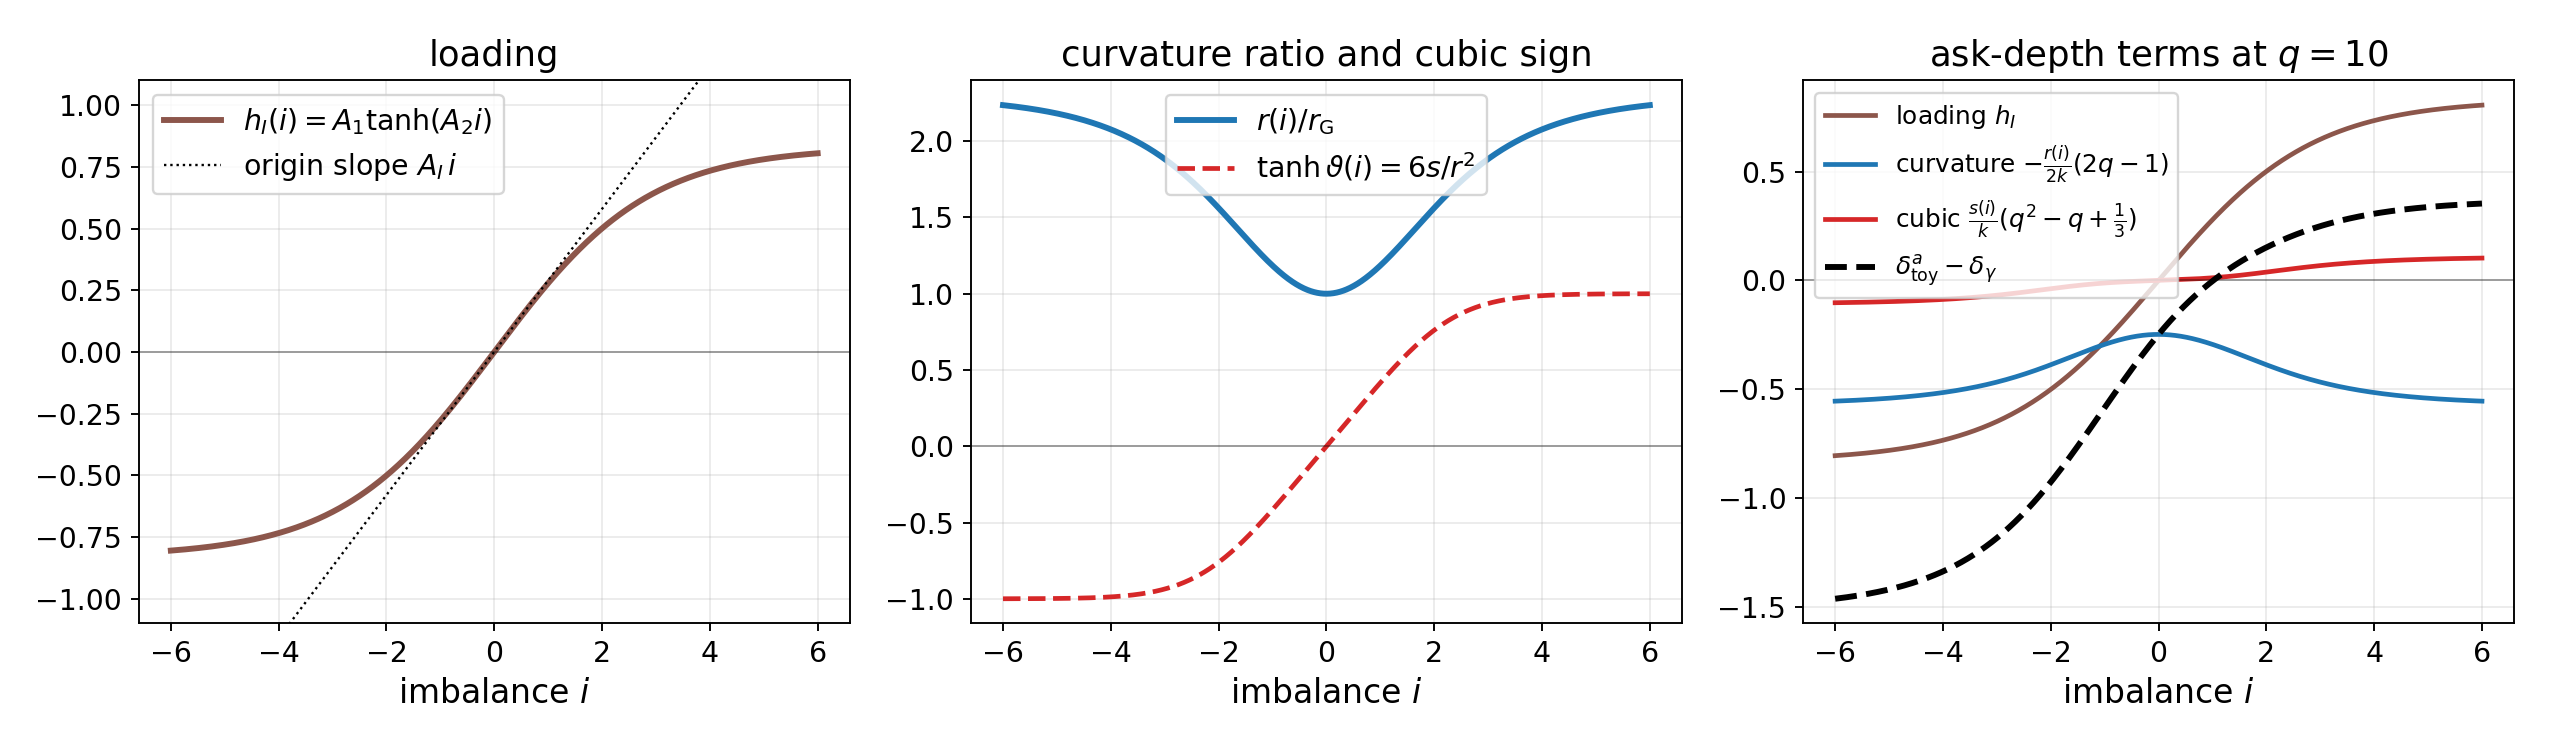
\includegraphics[width=\linewidth]{toy_closed_form_anatomy.png}
\caption{Ingredients of the toy closed form \eqref{eq:toy_curvature_quotes}
at the baseline parameters.  Left: the saturating loading \(h_I\)
\eqref{eq:toy_loading_ansatz} against its origin slope \(A_Ii\).  Middle: the
curvature ratio \(r(i)/r_{\rm G}\) \eqref{eq:toy_explicit_curvature_main},
which reaches \(2.24\) at \(|i|=6\), and \(\tanh\vartheta(i)=6s(i)/r(i)^2\),
the sign and relative size of the cubic \eqref{eq:toy_curvature_rs}.  Right:
the three terms of the ask depth \(\delta^a_{\rm toy}-\delta_\gamma\) at
\(q=10\): loading, curvature \(-\tfrac{r(i)}{2k}(2q-1)\) and cubic
\(\tfrac{s(i)}{k}(q^2-q+\tfrac13)\).}
\label{fig:toy_closed_form_anatomy}
\end{figure}

\subsection{Toy Numerical Study}

The toy study uses the parameters of Table~\ref{tab:parameters}
(\(\beta=0.0125\), \(\eta=0.32\), \(\bar\Lambda=0.9\), \(k=2\), \(\gamma=0.01\),
\(\sigma=0.3\); \(q_{\max}=60\), \(121\) imbalance points on \([-6,6]\),
\(T=10000\), \(\Delta t=0.05\), \(20000\) paths).  These give
\(\tfrac{\gamma\sigma^2}{2}=0.00045\); the OU state has stationary standard
deviation \(\sqrt{\eta^2/2\beta}\approx2.02\) and half-life
\(\log2/\beta\approx55.5\).

\paragraph{Calibration.}
The values in Table~\ref{tab:parameters} are illustrative rather than
estimated: time is measured in units in which balanced flow brings
\(2\bar\Lambda=1.8\) market orders per unit, with \(\sigma=0.3\) in these units,
and the flow parameters are chosen so that the three time scales are well
separated (alpha half-life \(\log2/\zeta\approx2.8\), imbalance half-life
\(\log2/\beta\approx55\), mean regime dwell \(\tau_R=120\)) and the imbalance
channel is visible in the quotes: the stationary imbalance
\(\sqrt{\eta^2/2\beta}\approx2.0\) makes the buy share \(\tfrac12(1+\tanh I)\)
fall outside the band \([0.12,0.88]\) about \(62\%\) of the time (equivalently,
exceed \(0.88\) about \(31\%\) of the time), a deliberately strong asymmetry.
Remark~\ref{rem:calibration_local} reports how the elementary closures behave
away from this point; an empirical calibration of \((\beta,\eta)\) to
trade-sign autocorrelations is left for future work.

\begin{table}[htbp]
\centering
\caption{Model and simulation parameters used in the reported experiments.}
\label{tab:parameters}
\begin{tabular}{lll}
\hline
Symbol & Meaning & Value\\
\hline
\(\gamma\) & CARA risk aversion & \(0.01\)\\
\(\sigma\) & reference-price volatility & \(0.3\)\\
\(\bar\Lambda\) & base market-order intensity & \(0.9\)\\
\(k\) & fill-intensity depth decay & \(2\)\\
\(\beta\) & imbalance OU mean reversion & \(0.0125\)\\
\(\eta\) & imbalance OU volatility & \(0.32\)\\
\(\zeta\) & alpha mean reversion & \(0.25\)\\
\(\epsilon\) & alpha flow-jump size & \(0.005\)\\
\(\eta_\alpha\) & alpha diffusion volatility & \(0.001\)\\
\(\tau_R\) & mean regime dwell time & \(120\)\\
\(z_{\pm1}\) & regime imbalance levels & \(\pm1.25\)\\
\(q_{\max}\) & inventory grid bound & \(60\)\\
\(I\)-grid & imbalance grid & \(121\) points on \([-6,6]\), \(\Delta i=0.1\)\\
\(T\) & simulation horizon & \(10000\)\\
\(\Delta t\) & simulation time step & \(0.05\)\\
\(\Delta t_{\rm rec}\) & diagnostic recording interval & \(1\)\\
paths & Monte Carlo paths & \(20000\)\\
\hline
\end{tabular}
\end{table}

\begin{table}[htbp]
\centering
\small
\caption{Policies compared in the numerical studies.  ``GLFT'' is throughout
the Gaussian continuum form, not the finite-grid eigenvector
\eqref{eq:glft_stationary_depths}.  The RHJB policies quote through the
optimal-quote map \eqref{eq:state_dep_recovery} applied to the ergodic relative
value of the stated equation; the \(I\)-aware RHJB has no alpha term, the
Alpha/\(I\)-aware RHJB is solved under a centred no-regime OU, and the
regime-aware RHJB takes \(R_t\) as perfectly observed---a full-information
benchmark, the target the regime closed forms approximate.  These names are
used in the result tables and figure legends below, abbreviated there by
dropping the ``signal-blind'', ``RHJB'' and study qualifiers where the column
width requires it.}
\label{tab:policies}
\begin{tabular}{llll}
\toprule
Policy & Observes & Quotes from & Study\\
\midrule
Signal-blind GLFT & \(q\) & \eqref{eq:glft_closed_ask}--\eqref{eq:glft_closed_bid} & all\\
\(I\)-aware RHJB & \(q,I\) & ergodic \eqref{eq:toy_ergodic} & all\\
Alpha/\(I\)-aware RHJB & \(q,I\) via \(\alphabar(I)\) & ergodic \eqref{eq:fast_alpha_ergodic} & \S\ref{sec:fast_alpha}, \S\ref{sec:regime}\\
Regime-aware RHJB & \(q,I,R\) & ergodic \eqref{eq:regime_ergodic_hjb} & \S\ref{sec:regime}\\
Toy self-consistent cubic & \(q,I\) & \eqref{eq:toy_curvature_quotes} & \S\ref{sec:toy}\\
Toy Galerkin-cubic & \(q,I\) & \eqref{eq:toy_galerkin_quotes} & \S\ref{sec:toy}\\
Fast-alpha hybrid cubic & \(q,I\) & \eqref{eq:fast_alpha_selfconsistent_quotes} & \S\ref{sec:fast_alpha}\\
Fast-alpha Galerkin-cubic & \(q,I\) & \eqref{eq:fa_galerkin_quotes} & \S\ref{sec:fast_alpha}\\
Regime hybrid cubic & \(q,I,R\) & \eqref{eq:regime_sccubic_quotes} & \S\ref{sec:regime}\\
Regime Galerkin-cubic & \(q,I,R\) & \eqref{eq:regime_galerkin_quotes} & \S\ref{sec:regime}\\
\bottomrule
\end{tabular}
\end{table}

The policies compared are signal-blind Gaussian GLFT, the numerical
\(I\)-aware RHJB, and the two toy closed forms (Table~\ref{tab:policies}).  Since \(S_t\) is a martingale in
this model, any performance difference comes from inventory control under
asymmetric fills: signal-blind GLFT is evaluated in the same \(I\)-imbalanced
environment without observing \(I_t\).  This benchmark is the textbook GLFT
rule at the maker's own \((\gamma,\sigma)\), not the policy of a maker who
knows the model and filters \(I_t\) from its fills, so the gap to the
\(I\)-aware RHJB bounds the value of flow information from above.

The \emph{self-consistent cubic} closed form (Approximation~\ref{prop:toy_curvature})---the
dynamic-curvature quotes \eqref{eq:toy_affine_quotes}, built from the elementary
loading \(h_I\) \eqref{eq:toy_loading_ansatz} and the dynamic curvature \(r(i)\)
\eqref{eq:toy_dynamic_r_main}, with the higher-order cubic \(s(i)\) added---and
the offline global Galerkin loading of
Appendix~\ref{app:toy_refined} keep the same tilted-GLFT structure: the
self-consistent cubic form corrects the asymmetric inventory tails, while the Galerkin-cubic
loading tightens the imbalance-axis fit at some cost along the inventory axis.  Figure~\ref{fig:toy_ansatz_selected_q}
overlays the body self-consistent cubic closed form and the appendix Galerkin-cubic loading
on the numerical RHJB as functions of imbalance; the inventory-axis fit is
quantified in Appendix~\ref{app:toy_refined}.


\begin{figure}[htbp]
\centering
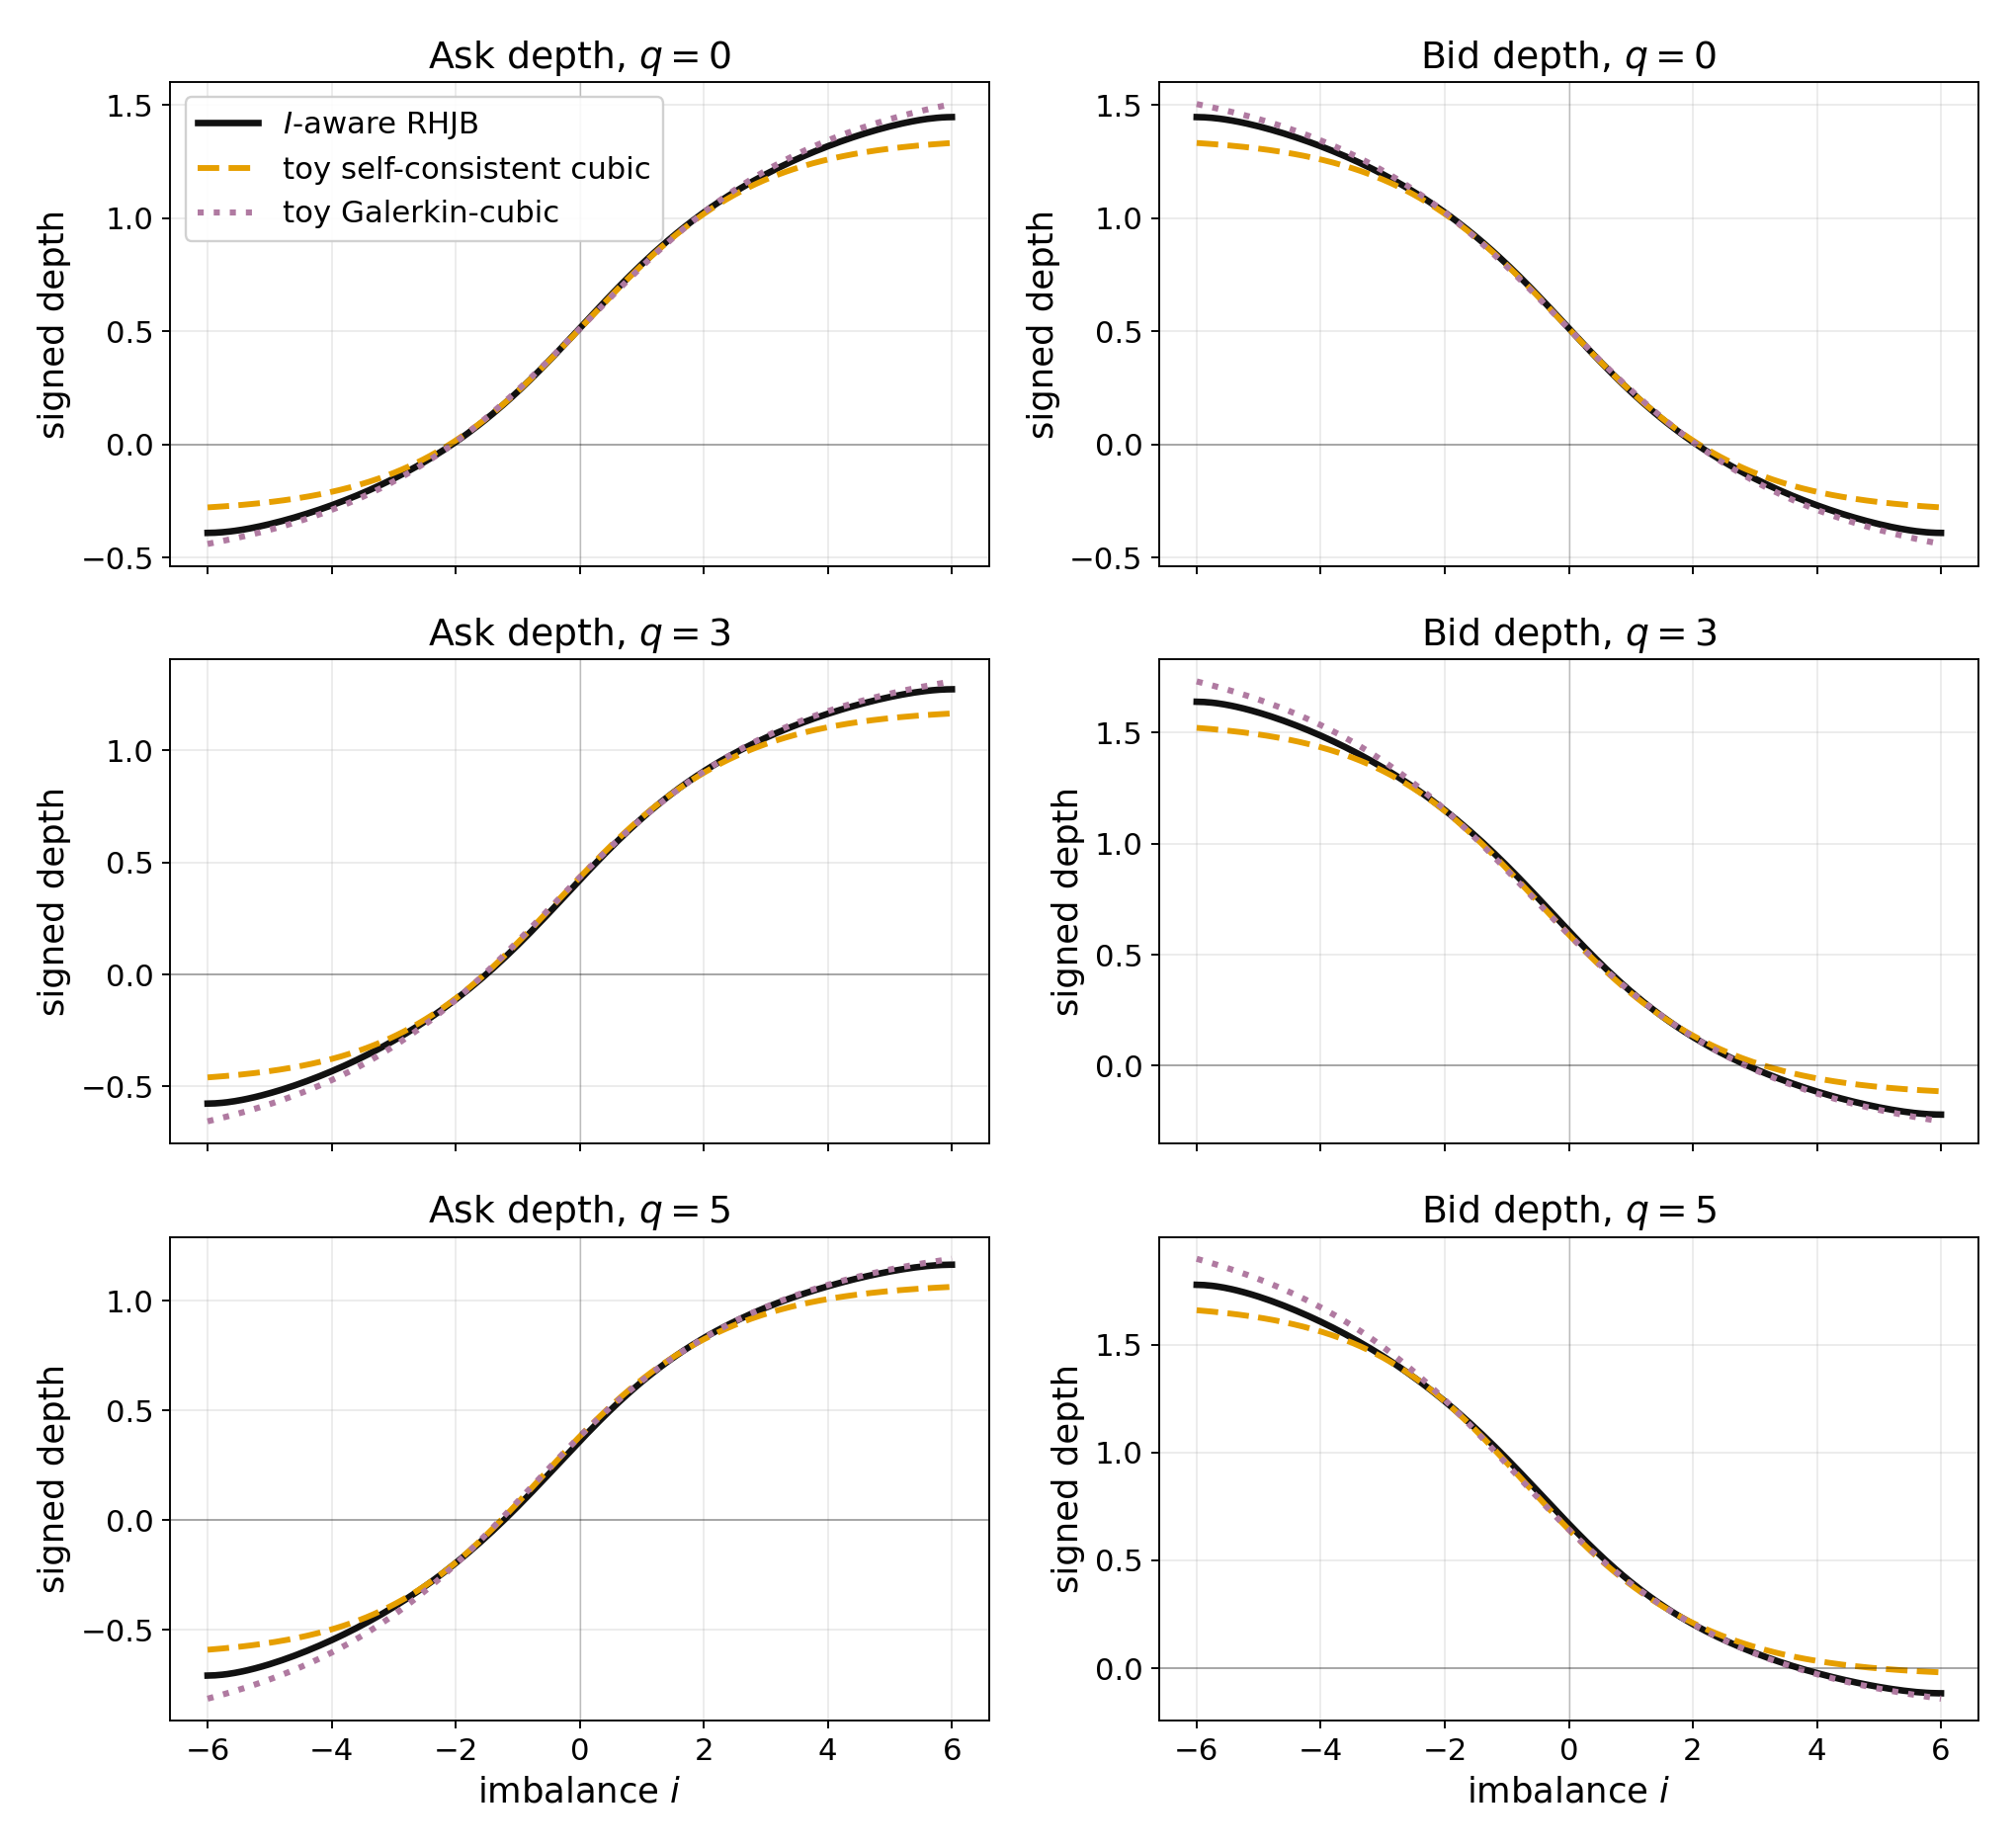
\includegraphics[width=0.85\linewidth]{cara_glft_yaware_ansatz_depths_vs_imbalance_v2.png}
\caption{Toy model quotes as functions of the imbalance value \(i\) at selected inventory values
(rows), overlaid on the numerical RHJB (solid): the body's self-consistent cubic closed
form \eqref{eq:toy_curvature_quotes} (dashed) and the global Galerkin loading of
Appendix~\ref{app:toy_refined} (dotted).}
\label{fig:toy_ansatz_selected_q}
\end{figure}

Terminal marked-to-market profit and loss is
\(\PnL_T:=X_T+Q_TS_T-(X_0+Q_0S_0)\).  The certainty equivalent reported in
Table~\ref{tab:toy_summary} is the sure PnL that the CARA maker regards as
equivalent to this random \(\PnL_T\),
\begin{equation}
\mathrm{CE}
=
-\frac1\gamma
\log
\E\left[\exp\{-\gamma \PnL_T\}\right],
\label{eq:certainty_equivalent}
\end{equation}
estimated from the terminal Monte Carlo sample.  By Jensen's inequality,
\(\mathrm{CE}\le\E[\PnL_T]\).  When the cumulant-generating function is finite
near the origin, the small-\(\gamma\) expansion gives
\(\E[\PnL_T]-\mathrm{CE}=\tfrac\gamma2\operatorname{Var}(\PnL_T)+O(\gamma^2)\);
the variance expression is therefore an approximation, not an identity.  The
exact CE in \eqref{eq:certainty_equivalent} incorporates all higher cumulants.

\begin{table}[htbp]
\centering
\begin{tabular}{lrrrrrr}
\toprule
Policy & Mean PnL & CE & Fills & \(\E|Q_t|\) & \(Q^{\rm life}_{.01}\) & \(Q^{\rm life}_{.99}\)\\
\midrule
Signal-blind GLFT & \(2407.65\) & \(953^{\dagger}\) & \(4812.56\) & \(15.53\) & \(-39\) & \(39\)\\
\(I\)-aware RHJB & \(2097.03\) & \(1842\pm6\) & \(3550.00\) & \(5.46\) & \(-13\) & \(14\)\\
Toy self-consistent cubic & \(2108.54\) & \(1834\pm12\) & \(3555.50\) & \(5.68\) & \(-13\) & \(13\)\\
Toy Galerkin-cubic & \(2095.17\) & \(1836\pm8\) & \(3540.05\) & \(5.55\) & \(-13\) & \(13\)\\
\bottomrule
\end{tabular}
\caption{Toy model Monte Carlo: \(20000\) paths, \(T=10000\), inventory grid
\([-60,60]\).  The price is a martingale, so \(I\)-aware policies harvest no
drift; their advantage is better control of flow-induced inventory exposure
and a higher CE.  \(\E|Q_t|\): path average of \(T^{-1}\int_0^T|Q_t|\,\dd t\);
\(Q^{\rm life}_{.01},Q^{\rm life}_{.99}\): 1st/99th inventory percentiles
pooled over paths and times; \(\pm\): one bootstrap standard error (SE) of CE
(200 path-level resamples).  Signal-blind GLFT sits far below
(\(\mathrm{CE}\approx950\), \(\E|Q_t|=15.5\)); the self-consistent cubic
\eqref{eq:toy_curvature_quotes} and appendix Galerkin loading both match the
numerical RHJB (\(\mathrm{CE}\) \(1834\)--\(1842\)) at \(\E|Q_t|\approx5.5\)
(\(\E[Q_t\mid I_t]\): Figure~\ref{fig:toy_inventory_cond_y}); paired on the
shared paths, \(\Delta\mathrm{CE}\) against the RHJB is \(-7.7\) (bootstrap SE
\(10.7\), \(95\%\) interval \([-29.5,12.9]\)) for the cubic and \(-5.9\)
(SE \(7.9\), \([-22.1,8.5]\)) for the Galerkin form.  (\(\dagger\))
Blind CE is tail-dominated and exploratory: exponential-weight effective
sample size (ESS) \(\approx8\) of \(20000\), batch variability \(\approx130\),
which a bootstrap SE cannot represent, so none is quoted; the
state-aware--blind ordering held in all ten contiguous \(2000\)-path batches
(state-aware ESS \(70\)--\(250\)).}
\label{tab:toy_summary}
\end{table}

\begin{figure}[htbp]
\centering
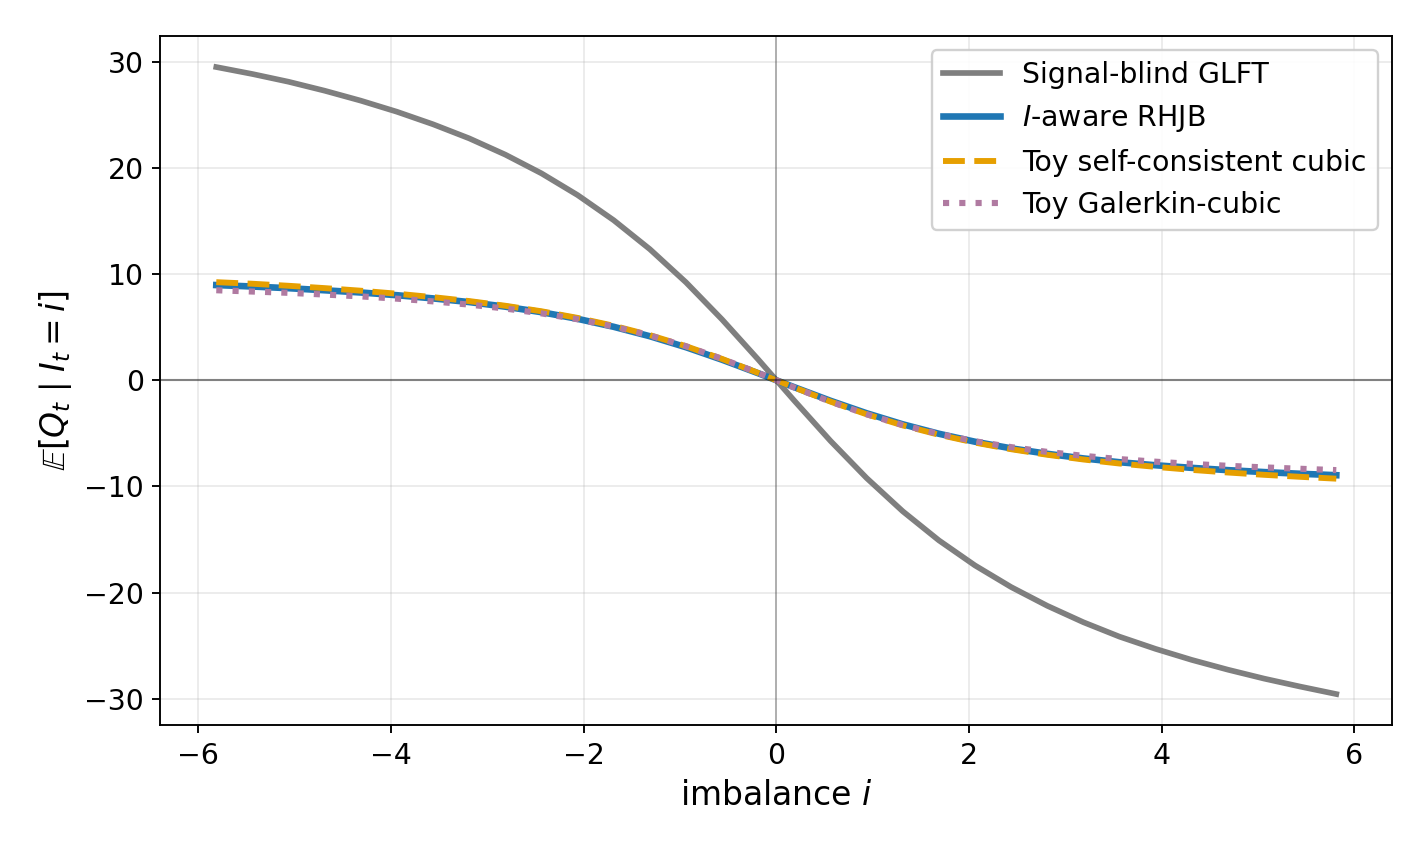
\includegraphics[width=0.7\linewidth]{cara_glft_expected_inventory_vs_y.png}
\caption{Toy model conditional inventory.  The plotted curves show
\(\E[Q_t\mid I_t]\) estimated over the \(20000\) simulated paths.  The
signal-blind GLFT policy is evaluated in the same imbalanced environment as
the \(I\)-aware policies; the body self-consistent cubic closed form
\eqref{eq:toy_curvature_quotes} and the appendix Galerkin loading both track the
numerical RHJB's conditional inventory closely, while directional flow pushes
the signal-blind GLFT inventory much farther away from zero.}
\label{fig:toy_inventory_cond_y}
\end{figure}


\section{Fast-Alpha Model}
\label{sec:fast_alpha}

\subsection{Simulation Environment}

The fast-alpha model keeps the same imbalance process \(I_t\), but now the
reference price has an explicit short-term drift:
\begin{equation}
\dd S_t=\alpha_t\,\dd t+\sigma\,\dd W^S_t.
\label{eq:alpha_price}
\end{equation}
This model captures the adverse-selection channel created when directional
order flow carries short-lived price information; see
\cite{CarteaJaimungalRicci2014,CarteaJaimungal2015,CarteaJaimungalPenalva2015,CarteaDonnellyJaimungal2018}
for related market-making models with predictive signals.  The difference here
is that the signal is not exogenous: the same imbalance state \(I_t\) that
skews the fill composition also generates the drift.  The drift state is
\begin{equation}
\dd\alpha_t
=
-\zeta\alpha_t\,\dd t
+\eta_\alpha\,\dd W^\alpha_t
+\epsilon\,\dd M_t^a
-\epsilon\,\dd M_t^b,
\label{eq:alpha_full_sde}
\end{equation}
with mean-reversion rate \(\zeta>0\), diffusive volatility \(\eta_\alpha\ge0\),
per-order jump size \(\epsilon>0\), and \(M^a,M^b\) the exogenous aggregate
market-order counts, Cox processes of intensities \(\Lambda^{a,0}(I_t)\),
\(\Lambda^{b,0}(I_t)\) constructed from the primitives of
Section~\ref{sec:setup} by
\(M_t^\ell=\int_{(0,t]}\!\int_{\R_+}\mathbf 1_{\{z\le\Lambda^{\ell,0}(I_s)\}}\,
\Pi^{M,\ell}(\dd s,\dd z)\).  Writing
\(\dd M_t^\ell=\dd\widetilde M_t^\ell+\Lambda^{\ell,0}(I_t)\,\dd t\) separates
martingale shocks from the predictable trend,
\begin{equation}
\E[\dd\alpha_t \mid \Fcal_t] = \Bigl( -\zeta\alpha_t+\epsilon\bigl(\Lambda^{a,0}(I_t)-\Lambda^{b,0}(I_t)\bigr) \Bigr)\dd t.
\label{eq:alpha_expected_drift}
\end{equation}
Since the intensities depend only on the autonomous factor \(I_t\) and
\(\alpha_t\) does not feed back into \((I,M^\ell)\), the system
\((I,\alpha)\) is triangular with globally Lipschitz, linear-growth
coefficients and bounded jump rates, hence has a unique non-explosive strong
solution \cite{Protter2005,Applebaum2009}.  We adopt a small-maker,
reduced-form coupling: conditional on the current imbalance and posted quotes,
the maker fills \(N^\ell\) and the aggregate counts \(M^\ell\) are
independent---the common scale \(\Lambda^{\ell,0}(I_t)\) links their state
dependence, not their event times---so adverse selection is captured through
the common state \(I_t\) rather than by making a maker fill and an alpha jump
the same order event.

\subsection{Fast-Alpha Reduction}

\begin{approximation}[Fast-alpha quasi-stationary mean]
\label{prop:alpha_bar}
If \(\alpha_t\) mean-reverts much faster than \(I_t\), its \(I\)-conditional mean is
\begin{equation}
\E[\alpha_t \mid I_t=i] \approx \alphabar(i) := \frac{2\bar\Lambda\epsilon}{\zeta}\tanh i .
\label{eq:alpha_bar_fast}
\end{equation}
\end{approximation}

\begin{proof}
At leading order in the fast-\(\alpha\) limit we freeze the slow variable
\(I_t=i\).  Conditioning \eqref{eq:alpha_full_sde} on \(I_t=i\), the drift of \(\alpha_t\)
is \(-\zeta\,\E[\alpha_t\mid i]+\epsilon\bigl(\Lambda^{a,0}(i)-\Lambda^{b,0}(i)\bigr)\),
and \eqref{eq:lambda_plus_y}--\eqref{eq:lambda_minus_y} give
\(\epsilon(\Lambda^{a,0}(i)-\Lambda^{b,0}(i))=2\bar\Lambda\epsilon\tanh i\) (the
diffusion \(\eta_\alpha\dd W^\alpha_t\) has zero conditional mean).  Setting this
frozen-\(I\) drift to zero gives \eqref{eq:alpha_bar_fast}; corrections from the
slow motion of \(I_t\) are of order \(\beta/\zeta\) and \(\eta^2/\zeta\).
\end{proof}

\begin{remark}[The frozen-\(I\) drift and its robustness]
\label{rem:frozen_i_robustness}
Equation~\eqref{eq:alpha_bar_fast} is the \emph{frozen-\(I\)} closure: the
\(I\)-conditional mean of \(\alpha\) with \(I\) held fixed over the fast
lifetime of \(\alpha\).  The exact stationary conditional mean is the bounded
odd solution of the resolvent equation
\[
(\zeta-\Lcal_I)\,m_\alpha(i)=2\bar\Lambda\epsilon\tanh i,\qquad
\Lcal_I=-\beta i\,\partial_i+\tfrac{\eta^2}{2}\partial_{ii},
\]
whose slope at the origin, \(m_\alpha'(0)\approx0.028\), is about \(23\%\)
below \(2\bar\Lambda\epsilon/\zeta=0.036\) (Figure~\ref{fig:alphabar_vs_exact}).  As \(m_\alpha\) is a discounted
Gaussian average of \(\tanh\) (its derivative one of \(\operatorname{sech}^2\)),
not elementary in general, we keep the frozen-\(I\) source as the leading-order
closure of the paper's minimal elementary architecture; richer elementary or
semi-closed refinements are not pursued.  The RMS difference between stationary
RHJB depths under \(\alphabar\) and \(m_\alpha\), pooled over both sides and
\(q\in\{-5,0,10,15\}\) and weighted by the OU stationary law
\(\pi_I=\mathcal N(0,\eta^2/2\beta)\), is \(\approx0.048\) depth units
(pointwise maximum \(\approx0.07\)), about \(9\%\) of the GLFT half-spread
\(\delta_\gamma+r_{\rm G}/(2k)\approx0.51\).  The \(23\%\) slope correction is
thus attenuated, not eliminated, in the posted depths; this is a depth
diagnostic and does not by itself establish robustness of the simulated PnL\@.
\end{remark}

\begin{figure}[htbp]
\centering
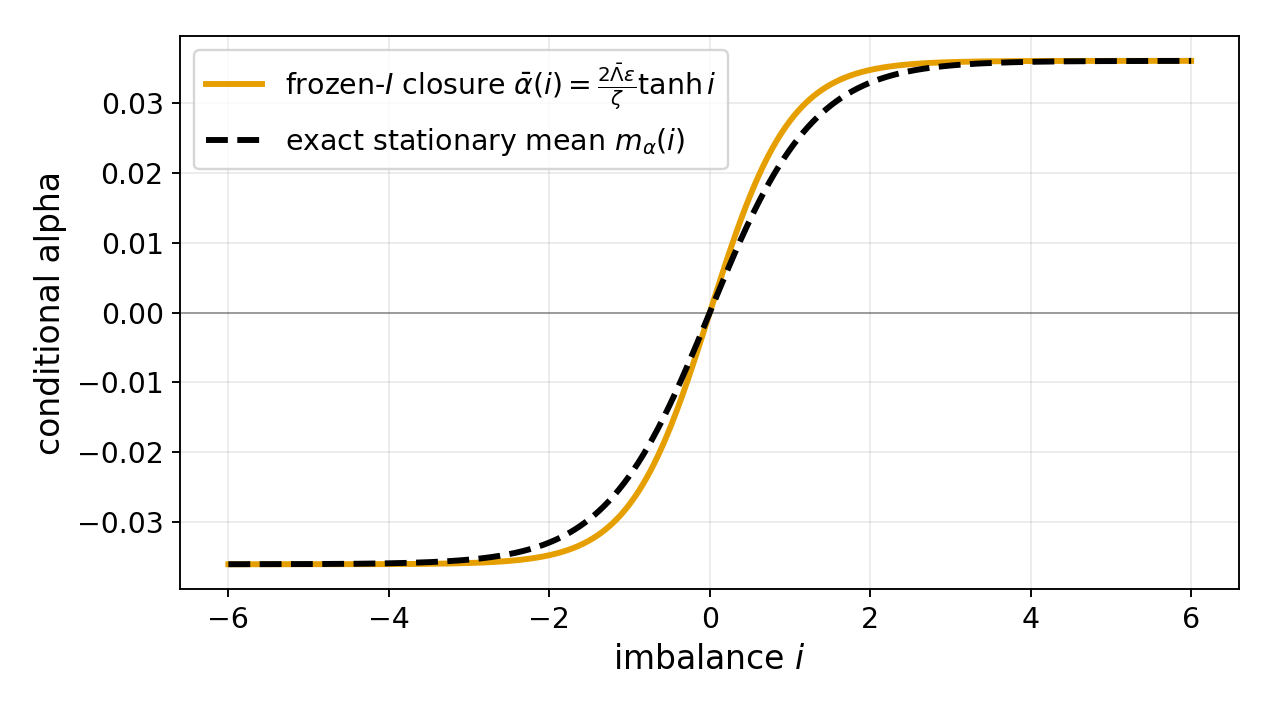
\includegraphics[width=0.6\linewidth]{alpha_frozen_vs_exact_mean.png}
\caption{The frozen-\(I\) closure \(\alphabar(i)\) \eqref{eq:alpha_bar_fast}
against the exact stationary conditional mean \(m_\alpha(i)\), the bounded odd
solution of the resolvent equation of Remark~\ref{rem:frozen_i_robustness}
(finite differences on \([-20,20]\)).  Both saturate at
\(2\bar\Lambda\epsilon/\zeta=0.036\); the OU diffusion smooths the transition,
lowering the origin slope from \(0.036\) to \(0.028\).}
\label{fig:alphabar_vs_exact}
\end{figure}

At the reported \(\zeta=0.25\) the alpha half-life \(\log2/\zeta\approx2.8\) is
twenty times shorter than the \(I\)-half-life \(55.5\)---the separation of time
scales that justifies using \(\alphabar(I_t)\) in the control equation while
retaining the full \(\alpha_t\) in the simulation.

\subsection{Fast-Alpha RHJB}

The full simulation state is \((X_t,S_t,Q_t,I_t,\alpha_t)\); the reported
control problem is solved instead in the \emph{surrogate model} in which the
reference-price drift is replaced by its frozen-\(I\) mean,
\(\dd S_t=\alphabar(I_t)\dd t+\sigma\dd W^S_t\), so that the state collapses to
\((X,S,Q,I)\).  Equation~\eqref{eq:fast_alpha_hjb} is the signal-risk-neutral
reduction of the exact CARA HJB of that surrogate.  It is neither the HJB of the
true \(\alpha\)-model nor the value function of an information-restricted
subclass of \(\Acal\): under \((Q,I)\)-feedback with the true \(\alpha\)-dynamics
the value function is not \((Q,I)\)-Markov, since \(\alpha_t\) still predicts
future \(S\).  The surrogate policies are then \emph{evaluated} on the fully
simulated system, and the depth cost of the substitution is the RMS reported
next.  An exploratory three-state
signal-risk-neutral ergodic solve in \((q,i,\alpha)\) (diffusion surrogate for
the alpha jumps) differs from the frozen-\(I\) policy by a depth RMS of
\(\approx0.06\), about \(12\%\) of the half-spread and the same order as the
other closure effects above---consistent with the residual
\(\alpha-\E[\alpha\mid I]\) carrying \(\approx17\%\) of the alpha variance but
reverting \(\zeta/\beta=20\) times faster than the imbalance; we do not pursue
the full-dimensional HJB further.  The fast-alpha policy uses the same
signal-risk-neutral reduction as \eqref{eq:toy_hjb}
(Remark~\ref{rem:srn_size} below quantifies the dropped term
\(-\tfrac{\gamma\eta^2}{2}(\partial_iu_q)^2\)) and adds the drift-reward term \(q\alphabar(i)\):
\begin{align}
\partial_\tau u_q
={}&
\Lcal_I u_q
+q\alphabar(i)
-\frac{\gamma\sigma^2}{2}q^2
\notag\\
&+
\frac{\Lambda^{a,0}(i)}{k}
\chi_\gamma
\exp\{k(u_{q-1}-u_q)\}
+
\frac{\Lambda^{b,0}(i)}{k}
\chi_\gamma
\exp\{k(u_{q+1}-u_q)\}.
\label{eq:fast_alpha_hjb}
\end{align}
The quotes are recovered from \(u\) by the unchanged map
\eqref{eq:state_dep_recovery}.
At fixed \(i\), the Cole--Hopf inventory step is
\begin{align}
\partial_\tau w_q
={}&
\left(kq\alphabar(i)-\frac{k}{2}\gamma\sigma^2q^2\right)w_q
\notag\\
&+
\chi_\gamma
\Lambda^{a,0}(i)w_{q-1}
+
\chi_\gamma
\Lambda^{b,0}(i)w_{q+1}.
\label{eq:fast_alpha_w}
\end{align}
The new diagonal term \(kq\alphabar(i)\) is the only difference relative to
the toy inventory block.  Economically, it makes inventory valuable when it is
aligned with the predicted price drift.

For fixed \(i\), the right-hand side of \eqref{eq:fast_alpha_w} defines the
fast-alpha inventory operator
\(\mathsf A_i^{\alpha}=\mathsf A_i^{\rm toy}+k\alphabar(i)\operatorname{diag}(q)\),
where \(\operatorname{diag}(q)\) has entries \(q\) in the ordered basis
\((-q_{\max},\ldots,q_{\max})\).  Spectrally, this asymmetric perturbation shifts the local principal eigenvector toward positive inventory when \(\alphabar(i)>0\) and toward negative inventory when \(\alphabar(i)<0\). This is the precise mathematical reason why the Alpha/\(I\)-aware policy carries directional inventory. By contrast, because the imbalance process \(I_t\) remains autonomous, its finite-difference generator matrix \(\mathsf L_I^\Delta\) is unchanged from the toy model.

Proposition~\ref{prop:toy_ergodic} applies verbatim: under the ergodic ansatz
\(u_q(\tau,i)=\lambda_{\alpha/I}\tau+c_{\alpha/I}+v_q(i)+o(1)\), normalized as
in Remark~\ref{rem:ergodic_existence}, the \(\tau\)-independent drift
\(q\alphabar(i)\) carries through and the pair \((\lambda_{\alpha/I},v)\)
solves
\begin{align}
\lambda_{\alpha/I}
={}&
\Lcal_Iv_q
+q\alphabar(i)
-\frac{\gamma\sigma^2}{2}q^2
+\frac{\Lambda^{a,0}(i)}{k}\chi_\gamma\exp\{k(v_{q-1}-v_q)\}
+\frac{\Lambda^{b,0}(i)}{k}\chi_\gamma\exp\{k(v_{q+1}-v_q)\},
\label{eq:fast_alpha_ergodic}
\end{align}
with quotes \(\delta^{a/b}=\delta_\gamma+v_q-v_{q\mp1}\).

\begin{remark}[Size of the dropped signal-risk term]
\label{rem:srn_size}
For the toy and fast-alpha models the exact CARA reduction is solved by the
same Strang scheme with the OU half-step applied to \(\psi=\e^{-\gamma u}\) (the
transform of \eqref{eq:regime_cara_joint_cole_hopf}), in which the signal-risk term is absorbed exactly.  On \(|i|\le6\),
\(q\in\{-5,0,10,15\}\), the signal-risk-neutral depths differ from the exact
CARA depths by an RMSE of \(0.044\) uniform / \(0.034\) stationary-weighted
(toy) and \(0.104\) / \(0.091\) (fast-alpha)---small in the toy, comparable to
the closed-form error itself in the fast-alpha model.  The same ordering holds
for the policies themselves.  Running the exact-CARA RHJB against the
signal-risk-neutral one on \(4000\) shared fast-alpha paths, the exact-CARA
policy holds less inventory (\(\E|Q_t|=5.95\) against \(7.19\)) and gives up
realized PnL---paired \(-137.3\pm2.6\), penalized \(-38.2\pm2.4\)---for a
certainty-equivalent difference indistinguishable from zero
(\(\Delta\mathrm{CE}=-7.4\), \(95\%\) bootstrap CI \([-49.7,32.8]\)): at
\(\gamma=0.01\) the signal-risk charge costs realized PnL without buying
measurable utility.  An elementary
leading-order correction, \(\sigma^2\to\sigma^2+\eta^2h'(i)^2\) in the
curvature \(r(i)\) of the closed forms below (\(h\) their imbalance loading),
improves the stationary-weighted fit of the fast-alpha closed form to the
exact-CARA depths (\(0.110\to0.064\)) but loses the GLFT collapse at \(i=0\)
(\(r(0)/r_{\rm G}\approx1.05\) toy, \(1.51\) fast-alpha) and, in a
\(20000\)-path paired Monte Carlo, quotes more conservatively
(\(\Delta\mathrm{PnL}=-139.7\pm0.6\)) with no detectable certainty-equivalent
gain (\(\Delta\mathrm{CE}=+7.7\), \(95\%\) bootstrap CI \([-3.5,18.5]\)).  The
SRN--CARA gap grows with \(\gamma\), and both elementary forms degrade once
\(r(i)\,q\) approaches unity, so this comparison is baseline-local; we retain
the signal-risk-neutral closed forms throughout.
\end{remark}

\subsection{Fast-Alpha Ansatz}

The ansatz keeps the GLFT curvature and adds a scalar signal loading,
\begin{equation}
v_q(i)\approx c(i)+q\bigl(A_{\rm flow}i+A_\alpha\tanh i\bigr)-\frac{r_{\rm G}}{2k}q^2 ,
\label{eq:fast_alpha_ansatz_value}
\end{equation}
where the flow composition and alpha drift are treated as independent additive effects.

\begin{approximation}[Fast-alpha local loading]
\label{prop:fast_alpha_loading}
Local matching of the ergodic RHJB \eqref{eq:fast_alpha_ergodic} near \(i=0\) yields the closed-form slopes
\begin{equation}
A_{\rm flow}=\frac{(2/k)\kappa}{\beta+2\kappa},
\qquad
A_\alpha=\frac{2\bar\Lambda\epsilon/\zeta}{\beta+2\kappa},
\label{eq:fast_alpha_closed_h}
\end{equation}
where \(2\kappa\) is the effective inventory-rebalancing rate from \eqref{eq:toy_glft_scales}.  The optimal-quote map then returns the closed-form affine quotes
\begin{align}
\delta_{\alpha/I,\mathrm{ans}}^a(q,i)
&=\delta_\gamma-\frac{r_{\rm G}}{2k}(2q-1)+A_{\rm flow}i+A_\alpha\tanh i,
\notag\\
\delta_{\alpha/I,\mathrm{ans}}^b(q,i)
&=\delta_\gamma+\frac{r_{\rm G}}{2k}(2q+1)-A_{\rm flow}i-A_\alpha\tanh i.
\label{eq:fast_alpha_ansatz_quotes_qY}
\end{align}
\end{approximation}

These affine quotes are the leading-order (\(i^1\)) form; the refinements below build on them.

\begin{proof}
Inserting the ansatz \(v_q=c+q\,h-\frac{r_{\rm G}}{2k}q^2\) into the ergodic RHJB \eqref{eq:fast_alpha_ergodic} and isolating the terms linear in \(q\) yields the matching condition
\[
\Lcal_I h(i)+\alphabar(i)+\frac{2c_{\rm GLFT}}{k\cosh i}\,r_{\rm G}\sinh\bigl(i-kh(i)\bigr)=0.
\]
We solve for the local slope by performing a first-order Taylor expansion around balanced flow (\(i=0\)). Since the profile is odd, \(h(0)=0\), so the function itself expands as \(h(i)\approx h'(0)i\). The terms expand as follows: the OU generator reduces to \(\Lcal_I h\approx-\beta i h'(i)\); the fast-alpha drift is \(\alphabar(i)\approx(2\bar\Lambda\epsilon/\zeta)i\); the prefactor \(1/\cosh i\) expands to \(1\); and the hyperbolic sine expands to \(\sinh\bigl(i-kh(i)\bigr)\approx i-kh'(0)i\). Substituting these and \(c_{\rm GLFT}r_{\rm G}=\kappa\) into the matching condition, the leading-order \(i^1\) terms obey
\[
-\beta h'(0)+\frac{2\bar\Lambda\epsilon}{\zeta}+\frac{2\kappa}{k}\bigl(1-kh'(0)\bigr)=0
\;\Longrightarrow\;
h'(0)=\frac{(2/k)\kappa+2\bar\Lambda\epsilon/\zeta}{\beta+2\kappa}.
\]
The shared denominator \(\beta+2\kappa\) reveals that the total slope is discounted by both the OU mean reversion (\(\beta\)) and the market-maker's own inventory rebalancing (\(2\kappa\)).  This origin slope \(h'(0)\) is exactly the sum \(A_{\rm flow}+A_\alpha\).
It is the slope of the \emph{locally affine} closure: the expansion
\(h\approx h'(0)i\) suppresses the cubic term that the diffusion acts on (for an
imposed \(\tanh\) shape, \(h'''(0)\neq0\) would add \(\eta^2\) to the
denominator).  Numerically, the exact solution of this matching condition has origin slope
\(\approx0.95\); the fuller appendix residual \eqref{eq:fa_loading_residual},
which carries the state-dependent curvature \(r(i)\) and the \(\e^{-r/2}\)
execution factor, gives \(\approx0.93\); and the measured RHJB skew slope at
\(q=0\) is \(\approx0.90\)---all below this local-affine value; the \(\tanh\) extension is
validated against the RHJB depths below rather than by the origin match.

To construct a global ansatz, we must extend this slope. Because the alpha drift globally follows \(\alphabar(i)\propto\tanh i\), its contribution is extended as \(A_\alpha\tanh i\). For the flow composition, imposing the saturated toy loading \(A_1\tanh(A_2 i)\) \emph{with the curvature frozen at \(r_{\rm G}\)} makes the flow term saturate early while the alpha term keeps growing, which mis-shapes the quotes at large imbalance; at this leading, curvature-frozen order we therefore keep the linear term \(A_{\rm flow}i\), and the quote map \(v_q-v_{q\pm1}\) recovers \eqref{eq:fast_alpha_ansatz_quotes_qY}.  The hybrid closure below can afford the saturating flow loading because its state-dependent curvature multiplier \(\mathcal M_I(i)\) grows with the same effective imbalance and restores the tail response that a frozen curvature loses.
\end{proof}

The leading-order quotes \eqref{eq:fast_alpha_ansatz_quotes_qY} freeze the
curvature at \(r_{\rm G}\) and keep the flow channel linear; they are the
scaffold of the derivation, not a separately reported model (the numerical
study below overlays only the cubic and Galerkin closed forms on the RHJB).
The body's working closed form is a saturating \emph{hybrid flow-gated
empirical cubic closure}---the \emph{hybrid cubic} for short---built on that
scaffold in three steps, with no fitted
or tuning constants; the architecture behind those steps was itself selected
against the RHJB (Remark~\ref{rem:architecture}).  The word \emph{empirical} describes the
architecture---which shift enters each coefficient---rather than parameter
fitting: every coefficient remains algebraic in the primitive model
parameters.  Unlike the toy local-equilibrium closure, it is not a
coefficient-by-coefficient match of one cubic value profile.

\paragraph{Flow-gated skew.}
Write the loading as the saturating toy flow loading plus the alpha-drift loading,
\begin{equation}
h_I(i)=A_1\tanh(A_2 i),\qquad h_\alpha(i)=A_\alpha\tanh i,\qquad A_2=\frac{\sqrt\beta}{\eta},
\label{eq:fa_selfcons_loadings}
\end{equation}
with \(A_\alpha\) the alpha slope of \eqref{eq:fast_alpha_closed_h} and
\(A_1\) the toy amplitude of Section~\ref{subsec:toy_curvature}.  The flow
channel uses the toy \emph{saturating} loading, whose origin slope
\(A_1A_2=\kappa/[k(\kappa+\beta)]\) folds in the OU-diffusion damping of the
\(\tanh\) profile and therefore sits below the bare local-linear slope
\(A_{\rm flow}\) of \eqref{eq:fast_alpha_closed_h} (\(0.290\) vs \(0.367\) at
the baseline); the hybrid cubic thus matches the affine leading order at
\(O(i^0)\) but not in the \(i^1\) flow slope.  The alpha channel extends the
local-linear coefficient \(A_\alpha=(2\bar\Lambda\epsilon/\zeta)/(\beta+2\kappa)\)
as a bounded \(\tanh\)---an extrapolation of the origin slope, not the
profile-consistent coefficient
\(A_\alpha\to(2\bar\Lambda\epsilon/\zeta)/(\beta+\eta^2+2\kappa)\) that applying
\(\Lcal_I\) to the full \(\tanh\) would give; we retain the local-linear
amplitude, which lies very close to the one-dimensional depth-RMSE optimum
against the RHJB, whereas the profile-consistent value underfits the alpha skew
markedly; this selection is one of the structural choices recorded in
Remark~\ref{rem:architecture}.  The state-dependent curvature deliberately reads the
\emph{flow-only} shift,
\begin{equation}
\vartheta_I(i)=i-k\,h_I(i),\qquad
\mathcal M_I(i)=\sqrt{\frac{\cosh i}{\cosh\vartheta_I(i)}},\qquad
r(i)=r_{\rm G}\,\mathcal M_I(i),
\label{eq:fa_selfcons_curv}
\end{equation}
and the skew gates the alpha weight from \(1\) at balanced flow to
\(\mathcal M_I\) in the saturated tail,
\begin{equation}
h_{\rm shift}(i)=\mathcal M_I(i)\,h_I(i)
+\bigl[1+g(i)\,(\mathcal M_I(i)-1)\bigr]\,h_\alpha(i),
\qquad g(i)=\tanh^2(A_2 i).
\label{eq:fa_selfcons_shift}
\end{equation}
This is a structural choice: the slope-subtracted toy closure applied to the
total loading would use \(\vartheta_{\rm full}:=i-kh_{\rm shift}\) and give
\(r_{\rm full}=r_{\rm G}\sqrt{\cosh i/\cosh\vartheta_{\rm full}}\), since
\(q\alphabar(i)\), though linear in \(q\), enters the execution exponent
through the loading; we do not impose it, and the reported flow-only
curvature is the empirical flow-gated choice evaluated below.

\paragraph{Hybrid full-shift cubic.}
Given the deliberately flow-only curvature, we retain the toy cubic functional
form as a separate \(q^3\)-inspired skew correction and evaluate its
hyperbolic factor at the \emph{full quoted shift}---the state the book
occupies given the reported skew---rather than at the flow shift
\(\vartheta_I\).  This does not restore strict \(q^2\) matching of a single
cubic profile:
\begin{equation}
\vartheta_{\rm full}(i)=i-k\,h_{\rm shift}(i),\qquad s(i)=\frac{r(i)^2}{6}\,\tanh\vartheta_{\rm full}(i).
\label{eq:fa_selfcons_cubic}
\end{equation}
For the baseline parameterization, the total skew slope at the origin exceeds the imbalance it offsets, \(k\bigl(h_I'(0)+h_\alpha'(0)\bigr)=k\,(A_1A_2+A_\alpha)>1\). Numerically, over the imbalance band the OU state populates, \(h_{\rm shift}\) has the same sign as \(i\) and \(\operatorname{sgn}(i)\,\bigl(h_{\rm shift}(i)-i/k\bigr)>0\); hence \(\vartheta_{\rm full}=i-k\,h_{\rm shift}\) carries the \emph{opposite} sign to \(i\) on that band, and the cubic \emph{opposes} the inventory tilt. This is exactly the sign of the residual \(q\)-convexity in the numerical fast-alpha RHJB (which is opposite to the bare toy cubic): evaluating \(s\) at \(\vartheta_I\) instead would reinforce the tilt and degrade the fit. The optimal-quote map \(v_q-v_{q\pm1}\) then returns the body's closed-form quotes
\begin{equation}
\boxed{\;
\begin{aligned}
\delta_{\alpha/I,\,\text{hybrid}}^a(q,i)&=\delta_\gamma+h_{\rm shift}(i)-\frac{r(i)}{2k}(2q-1)+\frac{s(i)}{k}\Bigl(q^2-q+\tfrac13\Bigr),\\[2pt]
\delta_{\alpha/I,\,\text{hybrid}}^b(q,i)&=\delta_\gamma-h_{\rm shift}(i)+\frac{r(i)}{2k}(2q+1)-\frac{s(i)}{k}\Bigl(q^2+q+\tfrac13\Bigr).
\end{aligned}\;}
\label{eq:fast_alpha_selfconsistent_quotes}
\end{equation}

\paragraph{Limit and empirical fidelity.}
At \(i=0\) both loadings vanish, so \(h_{\rm shift}=0\), \(\vartheta_I=\vartheta_{\rm full}=0\), \(r=r_{\rm G}\) and \(s=0\): the quotes collapse to the signal-blind GLFT form \eqref{eq:glft_closed_ask}--\eqref{eq:glft_closed_bid}, and no constant is fitted. Against the numerical RHJB the hybrid flow-gated cubic is the best-balanced closed form, with pooled ask\(+\)bid depth RMSE \(\approx0.096\) along the imbalance axis (on the \([-6,6]\) evaluation grid; wide-domain and stationary-weighted figures in Remark~\ref{rem:domain_convergence}) and \(\approx0.120\) along the inventory axis. The single-global-loading Galerkin-cubic variant of Appendix~\ref{app:fast_alpha_refined} lowers the inventory-axis RMSE to \(\approx0.105\) at the cost of the imbalance axis (\(\approx0.643\)); the body hybrid cubic is the balanced default.

Figure~\ref{fig:alpha_hybrid_anatomy} makes the closure visible: the flow
component \(\mathcal M_Ih_I\) and the gated alpha component of the skew; the
two effective imbalances, \(\vartheta_I\) growing with \(i\) while
\(\vartheta_{\rm full}\) has the opposite sign to \(i\) on all of \([-6,6]\),
as claimed above; the curvature multiplier and the gate; and the three terms
of the ask depth at \(q=10\).

\begin{figure}[htbp]
\centering
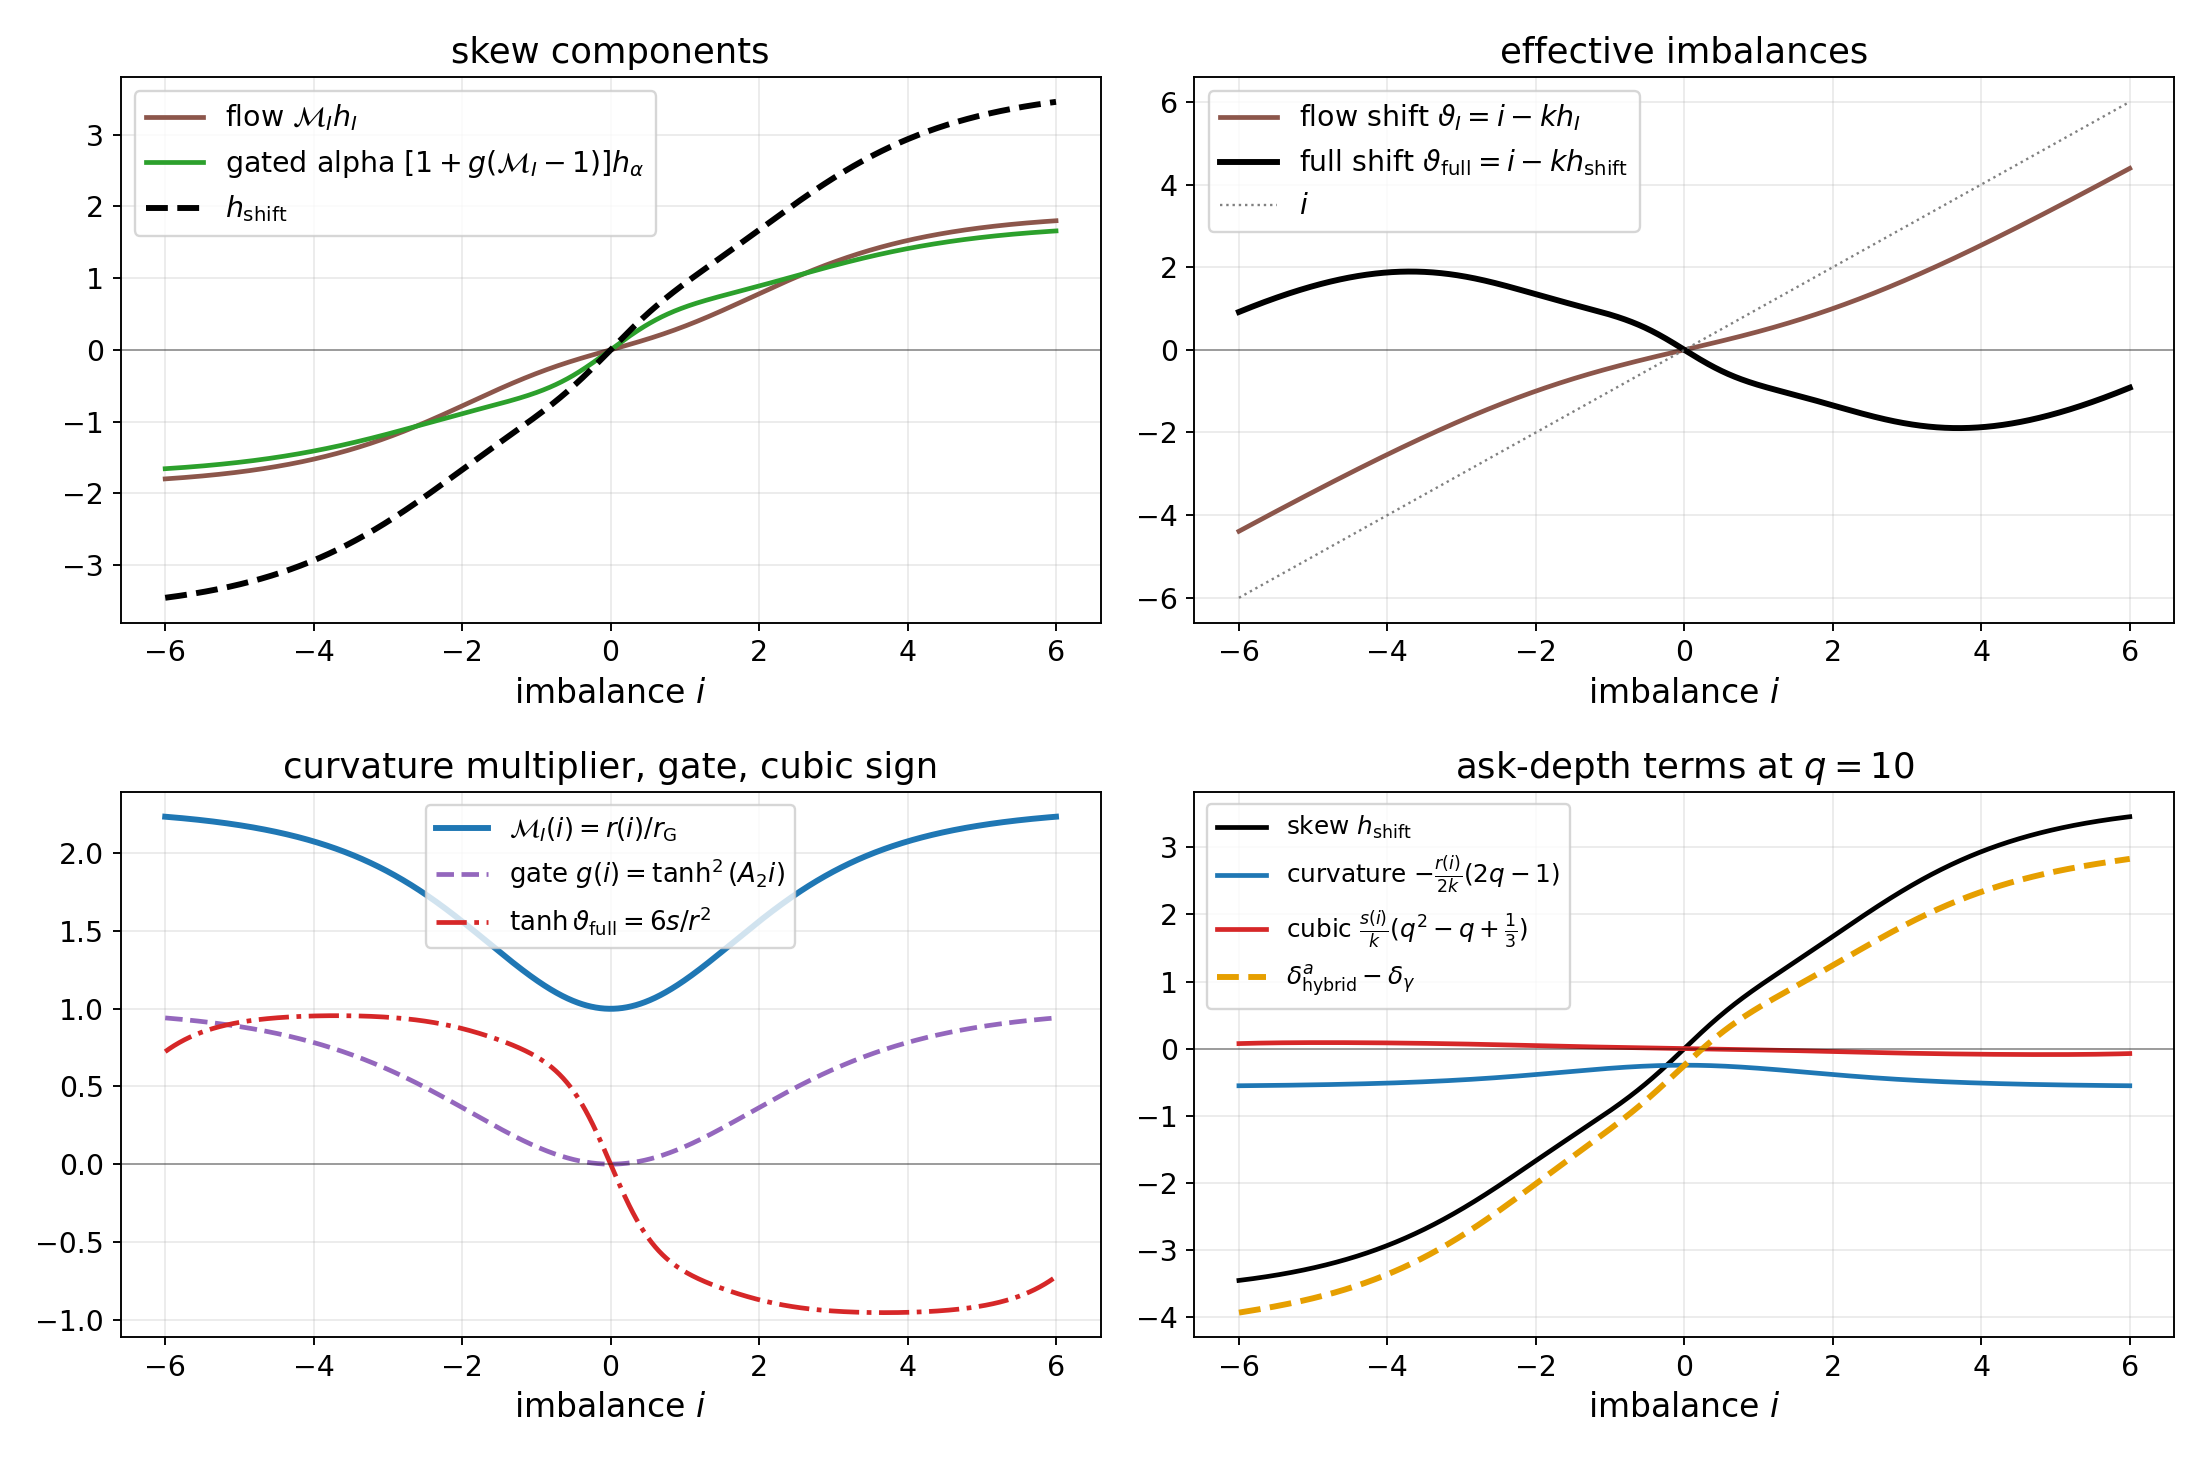
\includegraphics[width=0.9\linewidth]{alpha_hybrid_anatomy.png}
\caption{Ingredients of the hybrid flow-gated cubic
\eqref{eq:fast_alpha_selfconsistent_quotes} at the baseline parameters.  Top
left: the skew \(h_{\rm shift}\) \eqref{eq:fa_selfcons_shift} and its flow and
gated-alpha components.  Top right: the flow-only shift \(\vartheta_I\), which
the curvature reads, and the full shift \(\vartheta_{\rm full}\), which the
cubic reads and which has the opposite sign to \(i\) throughout
(\(k(A_I+A_\alpha)\approx2.1>1\)).  Bottom left: the curvature multiplier
\(\mathcal M_I\) \eqref{eq:fa_selfcons_curv}, the gate \(g\), and
\(\tanh\vartheta_{\rm full}=6s/r^2\).  Bottom right: skew, curvature and cubic
terms of the ask depth at \(q=10\).}
\label{fig:alpha_hybrid_anatomy}
\end{figure}

\begin{remark}[Architecture selection]
\label{rem:architecture}
The hybrid closure has no fitted scalar, but five structural choices---the
flow-only curvature \eqref{eq:fa_selfcons_curv}, the gate \(g\), the cubic
evaluated at the full shift \eqref{eq:fa_selfcons_cubic}, the local-linear
\(A_\alpha\), and, in Section~\ref{sec:regime}, the ungated regime
channel---were each fixed by comparing depth RMSE against the baseline RHJB.
The fidelity figures above are therefore in-sample with respect to that
selection; the frozen holdouts of Remark~\ref{rem:calibration_local} are the
out-of-sample check.
\end{remark}

\begin{remark}[Why the Alpha/\(I\)-aware policy carries more inventory]
\label{rem:why_carry_inventory}
Ignoring execution terms, the local tradeoff
\(q\alphabar(i)-\tfrac{\gamma\sigma^2}{2}q^2\) in the fast-alpha RHJB \eqref{eq:fast_alpha_hjb} has the
inventory target \(q^\star_{\rm d}(i)\approx\alphabar(i)/(\gamma\sigma^2)\),
which at saturated signal strength is
\(2\bar\Lambda\epsilon/(\zeta\gamma\sigma^2)=0.036/0.0009\approx40\) at the
baseline parameters---inside the \([-60,60]\) grid.  The alpha-aware policy
therefore intentionally carries directional inventory, posting
price-improving or marketable depths on one side when the signal is strong;
this is the economic content of the drift term, tempered in practice by the
execution channel (the realized lifetime quantiles stay near \([-16,16]\),
Table~\ref{tab:alpha_summary}) and controlled by \(\gamma\), \(\sigma\),
\(\epsilon\), or \(\zeta\).
\end{remark}

\subsection{Fast-Alpha Numerical Study}

The five policies compared---signal-blind Gaussian GLFT, the \(I\)-aware and
Alpha/\(I\)-aware RHJBs, the hybrid flow-gated cubic, and the Galerkin-cubic
form (Table~\ref{tab:policies})---are all evaluated under the full simulated
system \eqref{eq:alpha_price}--\eqref{eq:alpha_full_sde}, so the comparison
measures how well each converts the observable imbalance state into inventory
decisions when the realized drift follows the jump process; no policy observes
the realized \(\alpha_t\) path.  The study inherits every parameter of the toy
study (Table~\ref{tab:parameters}) and adds the alpha block \(\zeta=0.25\),
\(\epsilon=0.005\), \(\eta_\alpha=0.001\), whence the frozen-\(I\) drift proxy
has origin slope \(2\bar\Lambda\epsilon/\zeta=0.036\).  The depth figures
(Figures~\ref{fig:alpha_galerkin_ansatz_selected_q}
and~\ref{fig:alpha_galerkin_ansatz_vs_inventory}) compare stationary quoting
rules---the RHJB policies through
\eqref{eq:state_dep_recovery} applied to the ergodic values of
\eqref{eq:toy_ergodic} and \eqref{eq:fast_alpha_ergodic}, and the closed forms
\eqref{eq:fast_alpha_selfconsistent_quotes} and \eqref{eq:fa_galerkin_quotes};
the leading-order affine form \eqref{eq:fast_alpha_ansatz_value} only supplies
their local slopes and is not shown---so the Monte Carlo horizon affects only
the PnL and inventory diagnostics of Table~\ref{tab:alpha_summary}.

\begin{figure}[htbp]
\centering
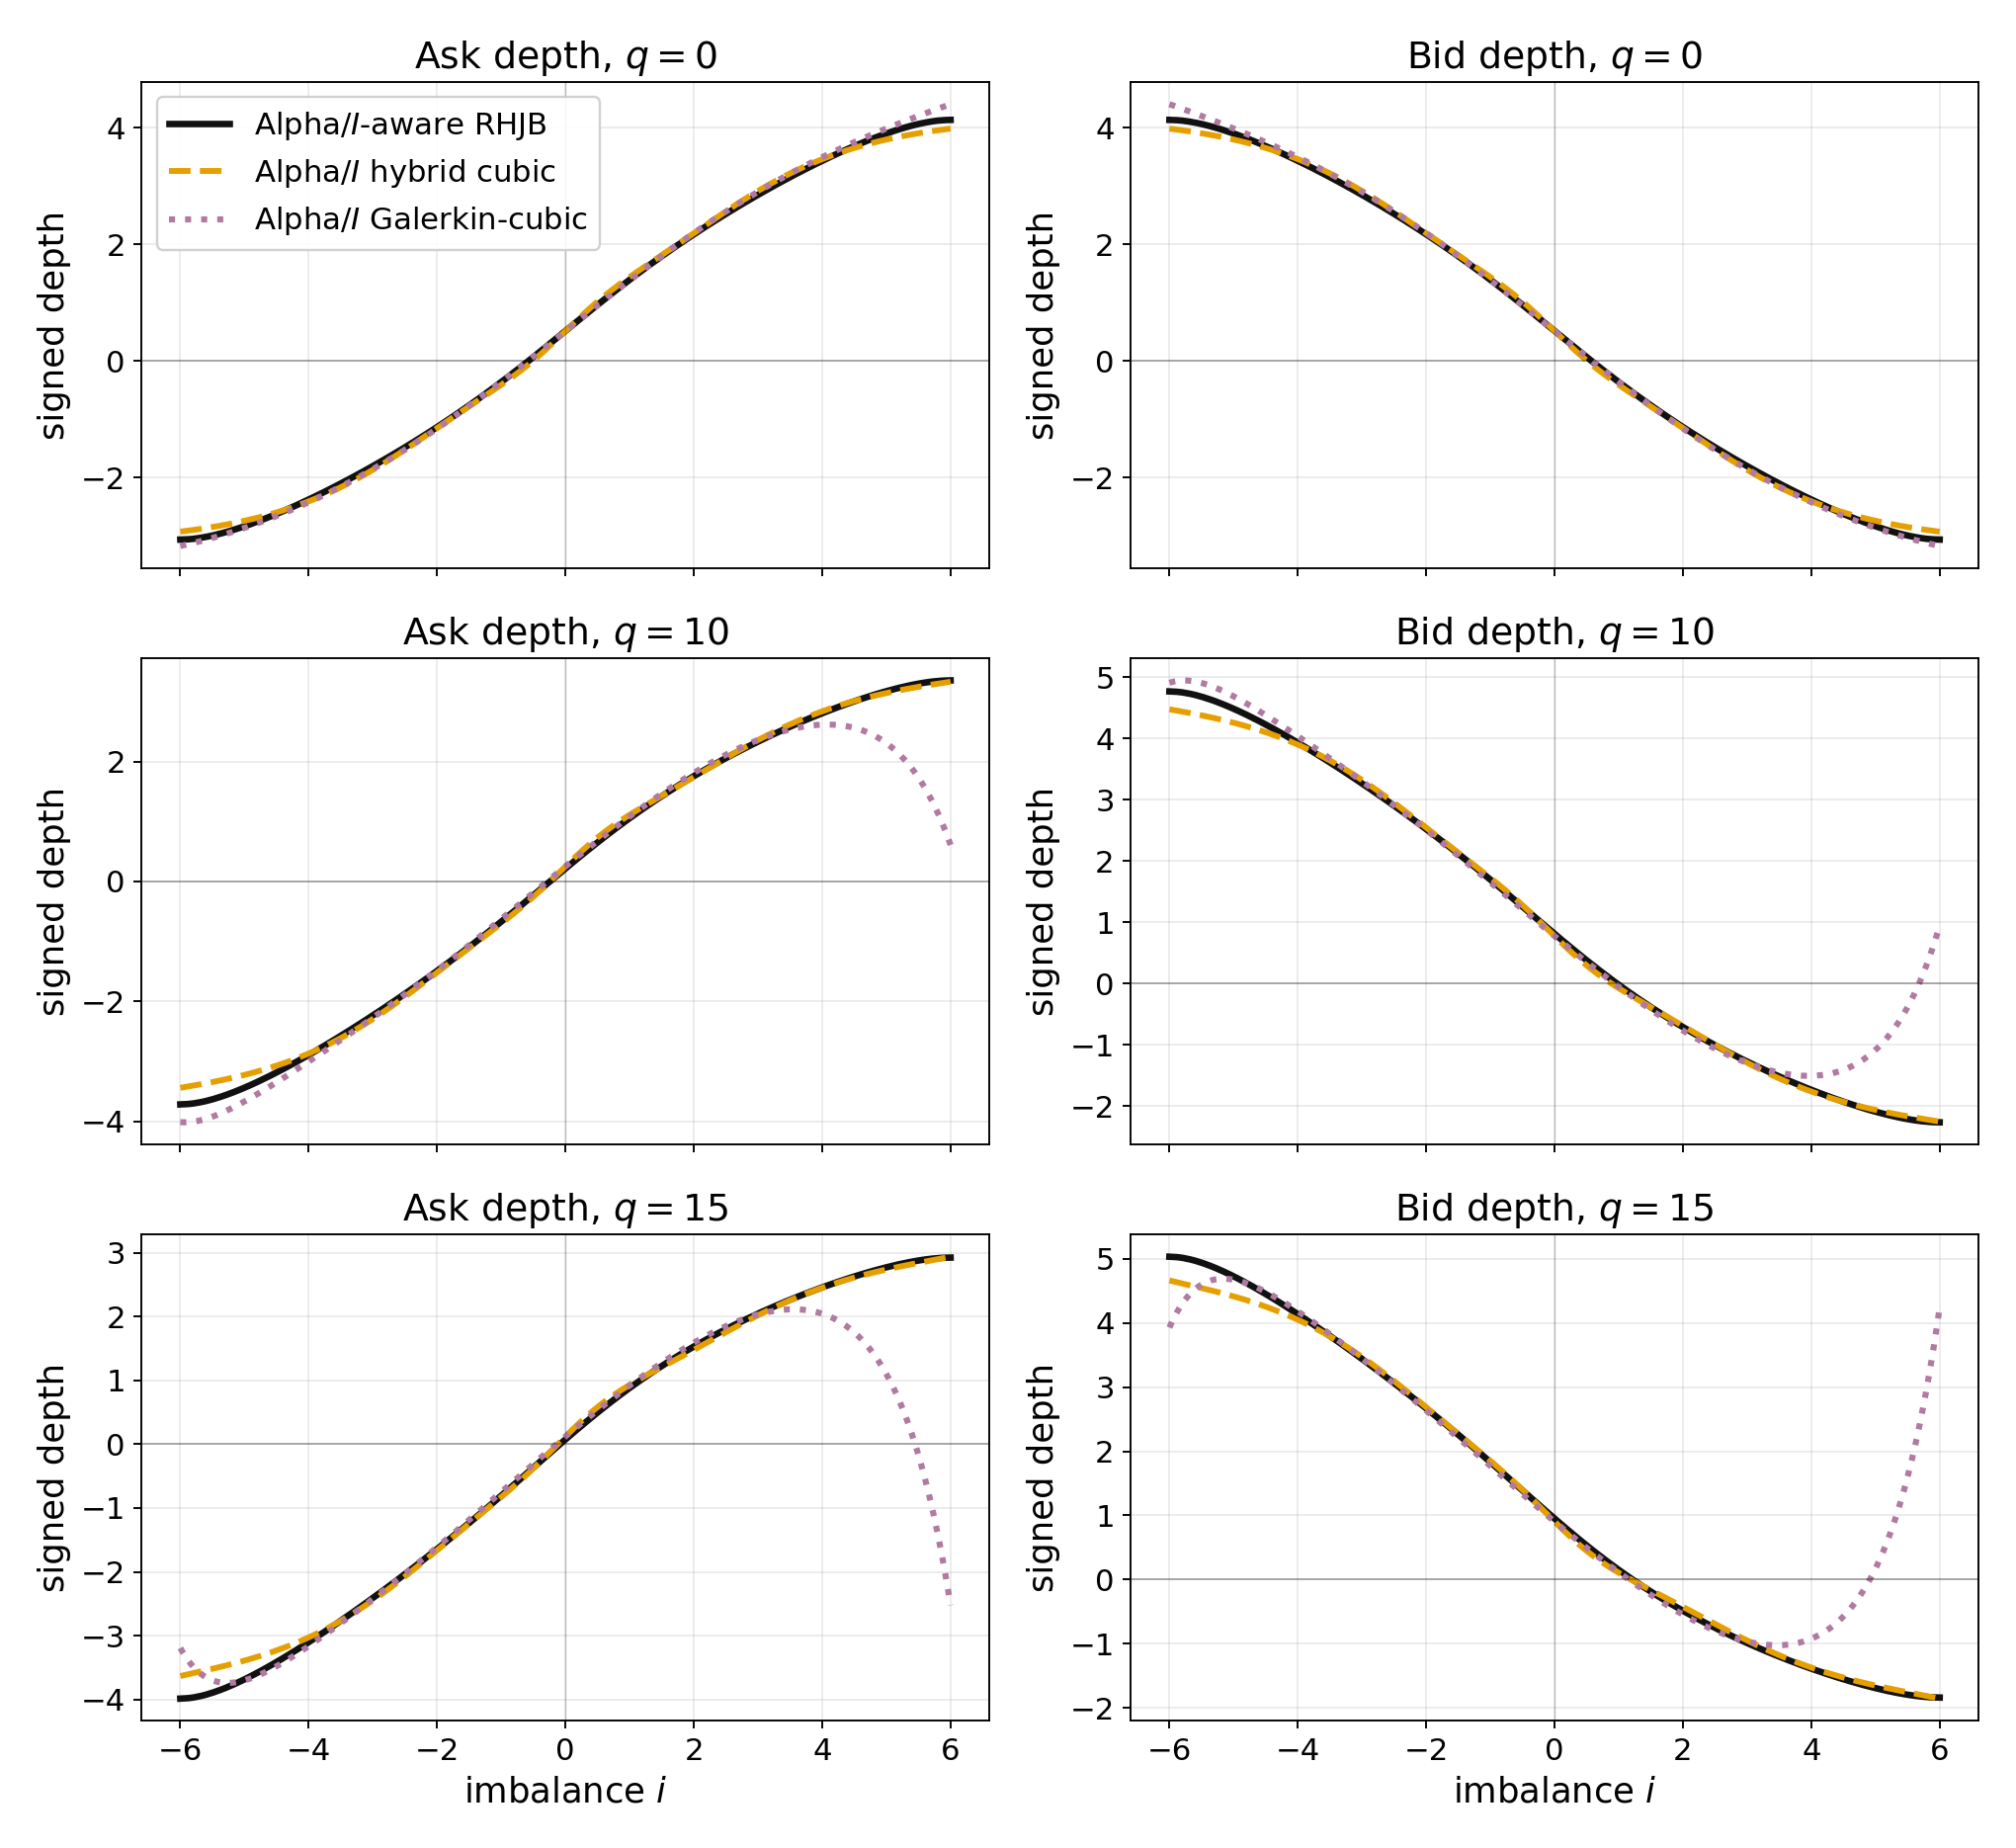
\includegraphics[width=0.85\linewidth]{alpha_reduced_galerkin_depths_vs_imbalance_v2.png}
\caption{Fast-alpha quotes as functions of the imbalance \(I\) at selected inventory values
(rows), overlaid on the numerical RHJB (solid): the body's hybrid flow-gated cubic
\eqref{eq:fast_alpha_selfconsistent_quotes} (dashed) and the appendix Galerkin-cubic form
\eqref{eq:fa_galerkin_quotes} (dotted). The hybrid cubic tracks the RHJB on both sides; the
single-loading Galerkin form deviates sharply in the imbalance tails at large inventory.}
\label{fig:alpha_galerkin_ansatz_selected_q}
\end{figure}

\begin{figure}[htbp]
\centering
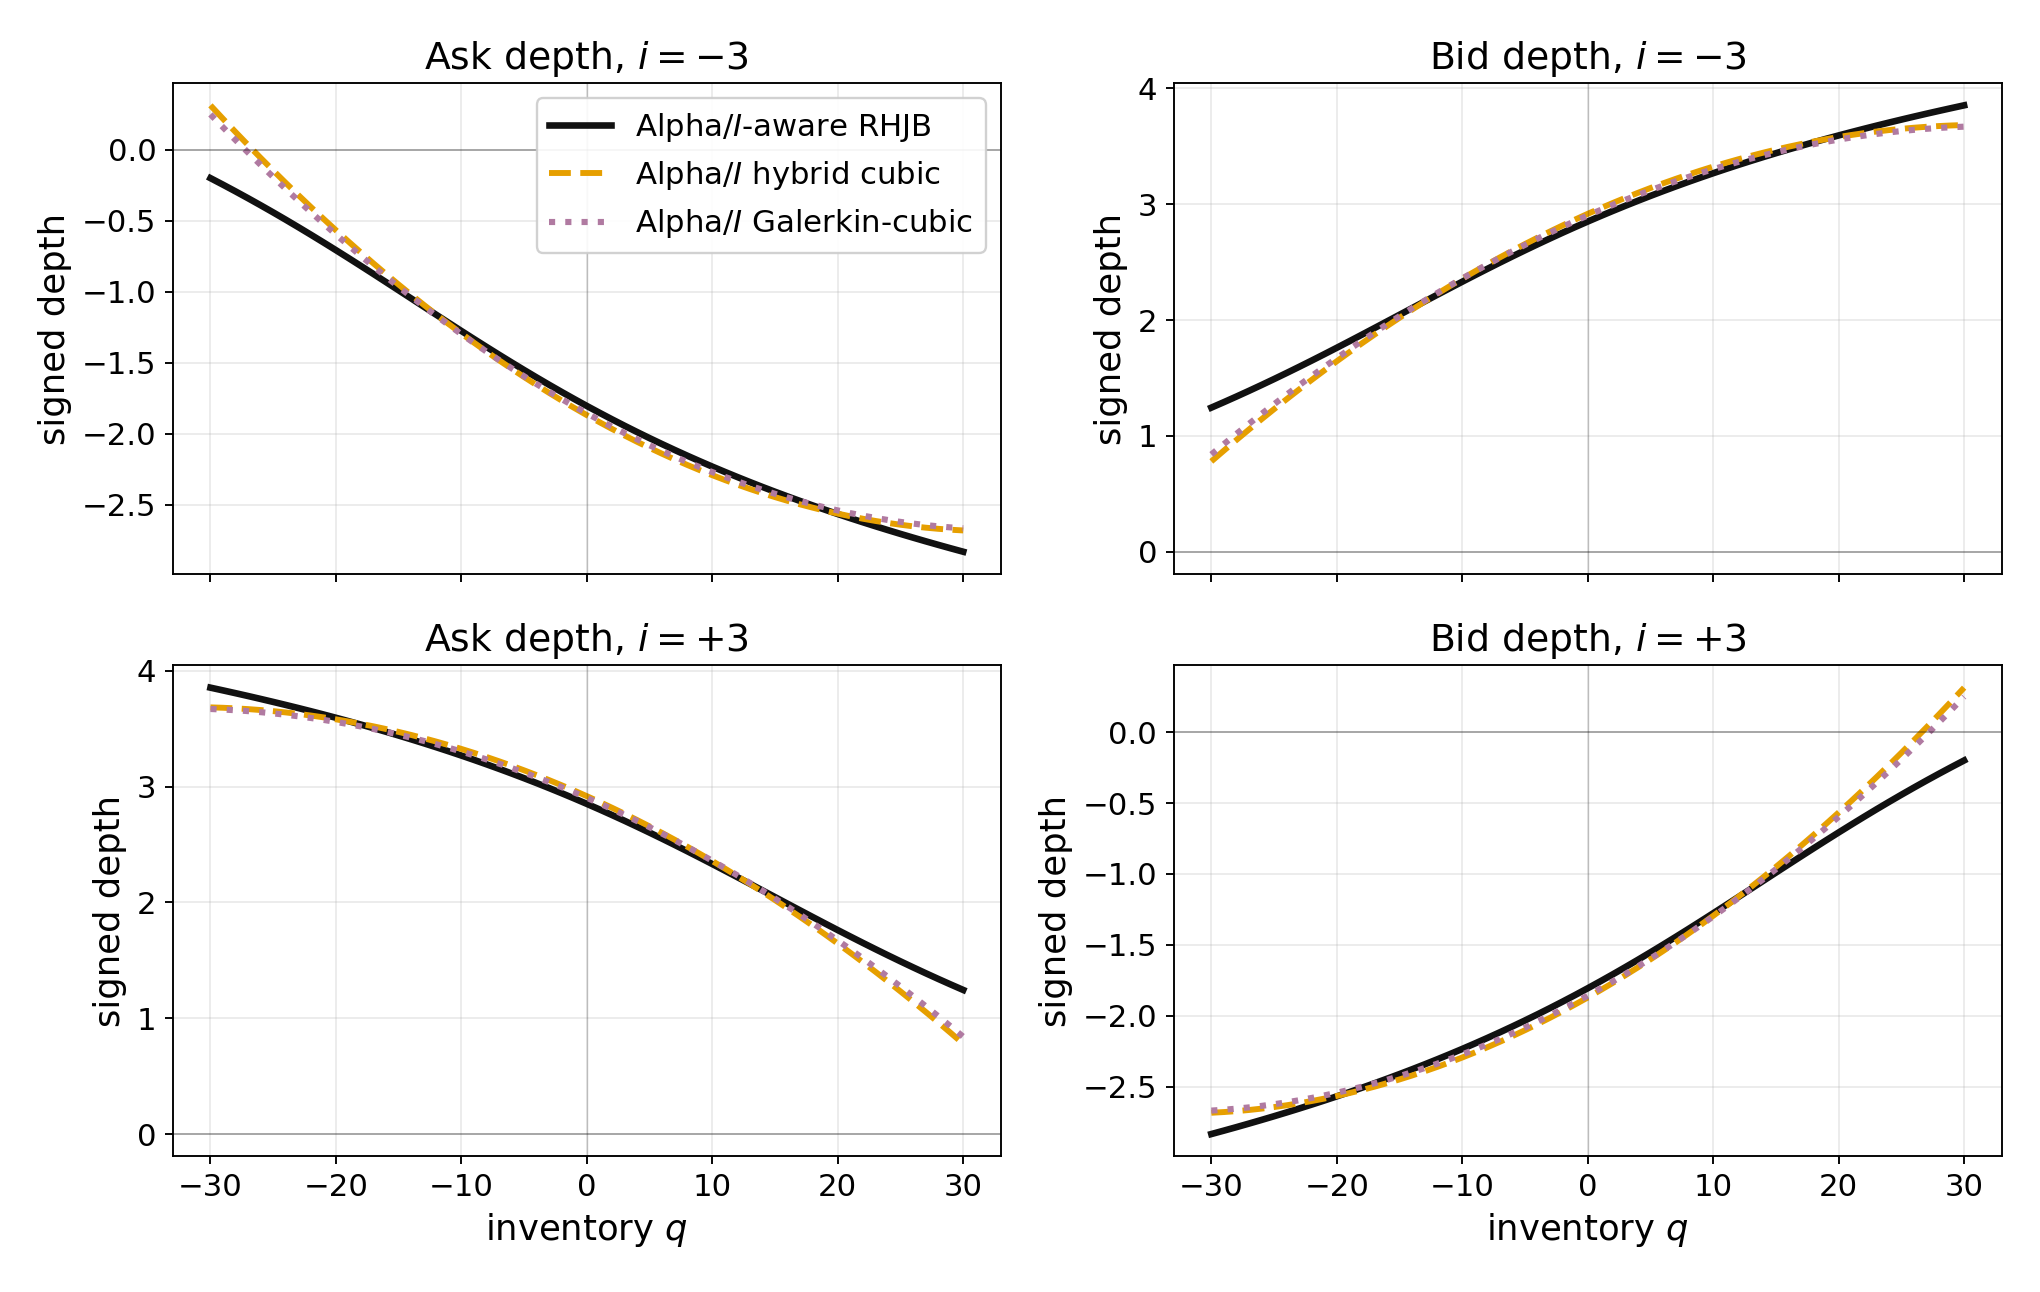
\includegraphics[width=0.85\linewidth]{alpha_reduced_galerkin_depths_vs_inventory_v2.png}
\caption{Fast-alpha quotes as functions of inventory at selected imbalance values,
overlaid on the numerical RHJB (solid): the body's hybrid flow-gated cubic
\eqref{eq:fast_alpha_selfconsistent_quotes} (dashed) and the appendix Galerkin-cubic form
\eqref{eq:fa_galerkin_quotes} (dotted). Here the single-loading Galerkin form attains the
tightest inventory-slice fit, with the hybrid cubic close behind. This is the inventory-slice
counterpart of Figure~\ref{fig:alpha_galerkin_ansatz_selected_q}.}
\label{fig:alpha_galerkin_ansatz_vs_inventory}
\end{figure}

Figure~\ref{fig:alpha_depth_error_vs_i} shows where the depth error lives:
for the hybrid cubic it is confined to \(|i|\gtrsim4\), where the stationary
law \(\pi_I\) carries little mass, so the stationary-weighted RMS
(\(0.045\)--\(0.055\) for \(q\in\{0,10,15\}\)) is well below the uniform one
(\(0.07\)--\(0.13\)); the Galerkin-cubic form is as accurate near the origin,
but its tail error at \(q=10,15\) reaches \(3\)--\(6\) depth units.

\begin{figure}[htbp]
\centering
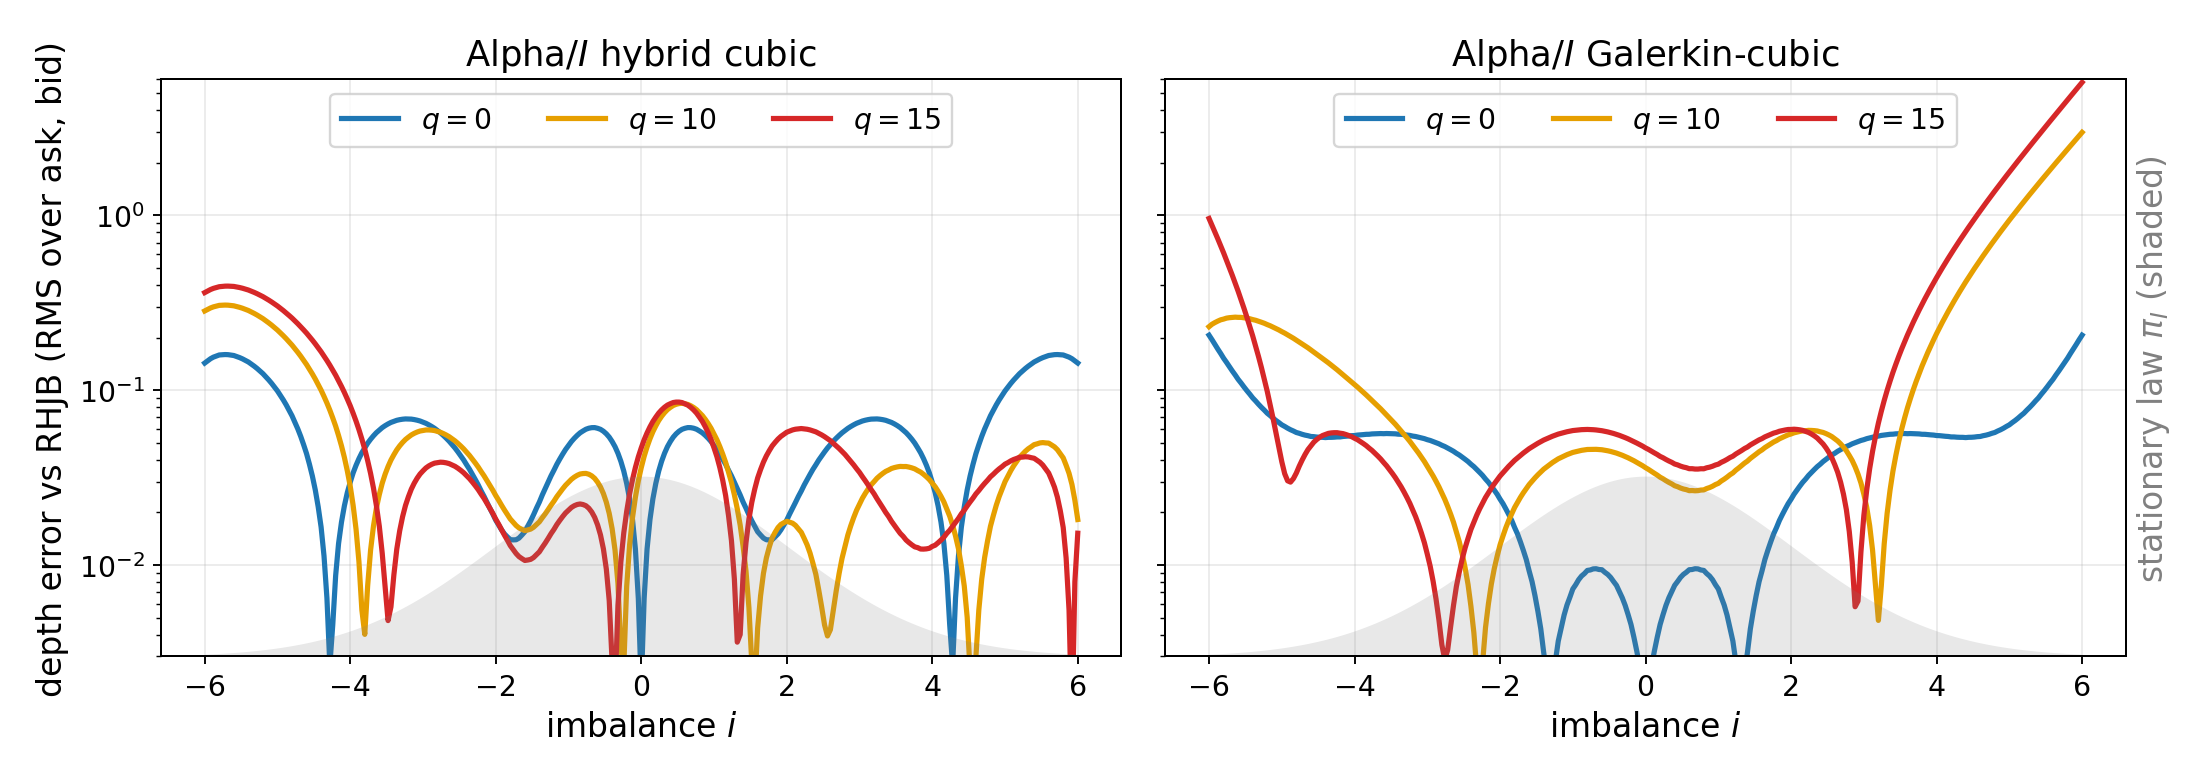
\includegraphics[width=0.95\linewidth]{alpha_depth_error_vs_i.png}
\caption{Fast-alpha depth error of the two closed forms against the numerical
RHJB along the imbalance axis (root mean square over ask and bid, log scale)
at \(q\in\{0,10,15\}\), with the OU stationary law \(\pi_I\) shaded.  The
hybrid cubic's error grows only outside the band \(\pi_I\) populates; the
Galerkin-cubic error explodes in the tails at large inventory (the plateau
mechanism of Appendix~\ref{app:fast_alpha_refined}).  This is the picture
behind the uniform-versus-weighted RMSE contrast of
Remark~\ref{rem:domain_convergence}.}
\label{fig:alpha_depth_error_vs_i}
\end{figure}


\begin{table}[htbp]
\centering
\setlength{\tabcolsep}{4.5pt}
\begin{tabular}{lrrrrrr}
\toprule
Policy & Total & Penalized & Spread & Alpha drift & \(\E|Q_t|\) & \(Q^{\rm life}_{.01},Q^{\rm life}_{.99}\)\\
\midrule
GLFT & \(-1945.91\) & \(-3527.26\) & \(2403.26\) & \(-4353.93\) & \(15.53\) & \([-39,39]\)\\
\(I\)-aware & \(667.69\) & \(473.57\) & \(2095.48\) & \(-1428.93\) & \(5.46\) & \([-13,14]\)\\
Alpha/\(I\)-aware & \(2513.67\) & \(2199.32\) & \(604.98\) & \(1910.82\) & \(7.19\) & \([-16,16]\)\\
Alpha/\(I\) hybrid cubic & \(2550.51\) & \(2198.48\) & \(522.51\) & \(2029.52\) & \(7.72\) & \([-16,16]\)\\
Alpha/\(I\) Galerkin-cubic & \(2521.16\) & \(2179.77\) & \(562.71\) & \(1960.30\) & \(7.53\) & \([-16,16]\)\\
\bottomrule
\end{tabular}
\caption{Fast-alpha Monte Carlo summary at the parameters of
Table~\ref{tab:parameters}.  Columns as in \eqref{eq:pnl_decomposition}:
Total is the realized PnL including the Brownian mark-to-market term, Alpha
drift is \(\E[\int_0^T Q_t\alpha_t\,\dd t]\), and Penalized is the diagnostic
\eqref{eq:penalized_pnl_diagnostic}; inventory metrics as in
Table~\ref{tab:toy_summary}.  Signal-blind GLFT earns spread but is adversely
aligned with the realized drift; observing \(I\) removes most of that adverse
selection, and using \(\alphabar(I)\) turns it into positive alpha-drift PnL
at the cost of more directional inventory.}
\label{tab:alpha_summary}
\end{table}

\paragraph{Paired contrasts.}
On the shared environment paths the penalized PnL of the hybrid flow-gated
cubic is statistically indistinguishable from the Alpha/\(I\)-aware RHJB's
(difference \(-0.8\), paired s.e.\ \(1.1\), \(95\%\) CI \([-2.9,1.3]\)), while
the Galerkin-cubic form trails it by \(-19.5\pm1.1\)
(Figure~\ref{fig:paired_ladder}); the other table entries
are path means over \(20000\) paths, reported without standard errors.

The Alpha/\(I\)-aware policies often post negative signed depths on one side
of the book---price-improving or marketable quotes that acquire directional
inventory (Remark~\ref{rem:why_carry_inventory}); the spread component
nonetheless remains positive on average, and the main gain comes from positive
alpha-drift PnL.

\begin{remark}[A recalibrated signal-blind benchmark]
\label{rem:blind_recalibration}
The first ladder step compares the state-aware policies with GLFT quoted at the
maker's own \(\sigma\).  Under persistent flow the maker's inventory is more
persistent, and more adversely aligned with the drift, than the signal-blind
model assumes, so part of that step reflects a mis-set inventory-risk parameter
rather than the value of observing \(I_t\).  Scaling only the quoting curvature,
\(r_{\rm G}\to m\,r_{\rm G}\), while holding the penalized diagnostic
\eqref{eq:penalized_pnl_diagnostic} at the true \(\gamma\sigma^2/2\), a
\(4000\)-path run on the fast-alpha environment gives
\[
\begin{array}{l|rrrrrrrrr}
m & 1 & 2 & 3 & 4 & 5 & 6 & 8 & 12 & 20\\\hline
\text{penalized} & -3509 & -1267 & -430 & +13 & +282 & +460 & +676 & +866 & +941\\
\E|Q_t| & 15.5 & 9.5 & 7.0 & 5.6 & 4.6 & 4.0 & 3.1 & 2.2 & 1.4
\end{array}
\]
against \(+478\pm5\) for the \(I\)-aware RHJB on the same paths (at \(m=1\) the
run reproduces the GLFT row of Table~\ref{tab:alpha_summary} within one standard
error).  A blind maker that only rescales its own risk parameter therefore
erases the ladder step by \(m\approx4\) and overtakes the \(I\)-aware RHJB
beyond \(m\approx6\) (paired difference \(+198\pm3\) at \(m=8\)).  Two caveats
keep this from being a like-for-like comparison.  The factor \(m\) is tuned in
sample on the diagnostic itself, whereas no state-aware policy is; and the
mechanism is inventory suppression rather than information, with \(\E|Q_t|\)
falling from \(15.5\) to \(1.4\) across the sweep, so that by \(m=20\) the maker
round-trips at marketable depths rather than making markets, a regime in which
the exponential fill law \eqref{eq:generic_fill_intensities} is no longer a
credible reduced form.  The first ladder step should nonetheless not be read as
the value of flow information under this diagnostic.  Under the CARA certainty
equivalent of Section~\ref{sec:toy}, where GLFT is admissible in the
signal-blind class, the upper-bound reading remains valid.
\end{remark}



\FloatBarrier

\section{Slow Regime Extension}
\label{sec:regime}

The toy and fast-alpha models use the current imbalance \(I_t\) as the only
flow signal, which cannot tell a positive \(I_t\) that is a short fluctuation
about to revert from one that reflects a persistent buy-pressure regime under
which future \(I\)-values will also stay positive.  The slow-regime extension
adds this distinction through a finite-state Markov chain \(R_t\) that shifts
the mean-reversion level of the OU imbalance process (the contrast with
\cite{GuilbaudPham2013} drawn in Section~\ref{sec:intro} applies: their chain
drives the cost of quoting, ours the future flow).  The simulated state is
\((X_t,S_t,Q_t,I_t,R_t,\alpha_t)\); the regime-aware RHJB keeps
\((Q_t,I_t,R_t)\) and eliminates \(\alpha_t\) by the fast mean
\(\alphabar(I_t)\) of Section~\ref{sec:fast_alpha}.

\subsection{Regime-Modulated Imbalance Process}
\label{subsec:regime_process}

Let \(\mathcal R\) be a finite set of regime labels.  The regime process
\(R_t\in\mathcal R\) is a
continuous-time Markov chain with generator
\[
\Gamma=(\nu_{rr'})_{r,r'\in\mathcal R},
\]
where
\[
\nu_{rr'}\ge0\quad(r'\ne r),
\qquad
\nu_{rr}=-\sum_{r'\ne r}\nu_{rr'}.
\]
Each regime \(r\) has an associated imbalance level \(z_r\in\mathbb R\).  The
imbalance process mean-reverts toward the current regime level:
\begin{equation}
\dd I_t
=
-\beta\bigl(I_t-z_{R_t}\bigr)\dd t+\eta\,\dd W^I_t.
\label{eq:regime_y_dynamics}
\end{equation}
When \(z_r>0\), the regime represents persistent buy pressure; when
\(z_r<0\), it represents persistent sell pressure; and when \(z_r=0\), it is a
neutral regime.  The regime chain is taken independent of the Brownian motions
and conditionally independent of the counting processes given the current
state.

In the reported experiments \(\mathcal R=\{-1,0,1\}\) with
\(z_{\pm1}=\pm1.25\), \(z_0=0\), and generator
\[
\Gamma
=
\begin{pmatrix}
-1/\tau_R & 1/\tau_R & 0\\
1/(2\tau_R) & -1/\tau_R & 1/(2\tau_R)\\
0 & 1/\tau_R & -1/\tau_R
\end{pmatrix},
\qquad
\tau_R=120,
\]
so the buy- and sell-pressure regimes pass through the neutral state before
switching sign, and the level vector \(z=(z_{-1},z_0,z_1)\) is an exact
eigenvector, \(\Gamma z=-(1/\tau_R)z\); the closed-form regime ansatz below
uses this eigenmode relation with \(\lambda_R=1/\tau_R\).

The zero-depth execution intensities remain
\eqref{eq:lambda_plus_y}--\eqref{eq:lambda_minus_y}, functions of the current
imbalance \(I_t\) alone: \(R_t\) does not enter the fill law directly, but
changes the conditional law of future \(I\)-values in
\eqref{eq:regime_y_dynamics}, so two paths with the same current \(I_t=i\) can
receive different quotes if their regimes imply different likely future
imbalance paths.

\subsection{Joint Generator}

For a vector-valued test function
\[
f(i,r)=f_r(i),
\qquad r\in\mathcal R,
\]
the generator of the joint \((I_t,R_t)\) process is
\begin{equation}
(\mathcal{L}_{I,R} f)_r(i)
=
-\beta(i-z_r)\partial_i f_r(i)
+\frac{\eta^2}{2}\partial_{ii} f_r(i)
+\sum_{r'\ne r}\nu_{rr'}\bigl(f_{r'}(i)-f_r(i)\bigr).
\label{eq:regime_joint_generator}
\end{equation}
The first two terms are the OU generator conditional on the current regime.
The last term is the Markov-chain switching generator.  It compares the value
in the current regime \(r\) with the value that would apply immediately after
a jump to another regime \(r'\).

The regime-aware policy uses the same GLFT-style reduction as the toy and
fast-alpha sections.  The exact CARA signal block contains the diffusion
signal-risk penalty \(-\tfrac{\gamma\eta^2}{2}(\partial_i u_{q,r})^2\) and the
nonlinear regime-switch term
\(\frac1\gamma\sum_{r'\ne r}\nu_{rr'}(1-\e^{-\gamma(u_{q,r'}-u_{q,r})})\).
Although nonlinear in \(u\), both are jointly absorbed by the same CARA
transform: with \(\psi_{q,r}=\e^{-\gamma u_{q,r}}\),
\begin{align}
(\mathcal L_{I,R}\psi_q)_r={}&-\gamma \psi_{q,r}\Bigg[
-\beta(i-z_r)\partial_i u_{q,r}+\frac{\eta^2}{2}\partial_{ii}u_{q,r}
-\frac{\gamma\eta^2}{2}(\partial_i u_{q,r})^2\notag\\[-2pt]
&\hspace{35mm}+\frac1\gamma\sum_{r'\ne r}\nu_{rr'}
\left(1-\e^{-\gamma(u_{q,r'}-u_{q,r})}\right)\Bigg].
\label{eq:regime_cara_joint_cole_hopf}
\end{align}
Thus the exact CARA signal subflow is linear in \(\psi\), with generator
\(\mathcal L_{I,R}\).  The RHJB below replaces this risk-sensitive block by
its signal-risk-neutral linearization \(\mathcal L_{I,R}u_q\), retaining the
inventory execution block in Cole--Hopf form; it is therefore an RHJB
benchmark, not the exact CARA HJB for the full regime-switching problem.

\subsection{Regime-Aware RHJB}

The regime-aware value correction is indexed by inventory and regime:
\[
u_{q,r}(\tau,i),
\qquad q\in\Qcal,\quad r\in\mathcal R.
\]
The regime RHJB retains the frozen-\(I\) alpha closure \(\alphabar(i)\) of
\eqref{eq:alpha_bar_fast} (Remark~\ref{rem:frozen_i_robustness}); this is not
the exact stationary mean \(\E[\alpha\mid I=i,R=r]\), which in the modulated
process generally also depends on \(r\).
The regime-aware RHJB is
\begin{align}
\partial_\tau u_{q,r}
={}&
(\mathcal{L}_{I,R} u_q)_r(i)
+q\alphabar(i)
-\frac{\gamma\sigma^2}{2}q^2
\notag\\
&+
\frac{\Lambda^{a,0}(i)}{k}
\chi_\gamma
\exp\{k(u_{q-1,r}-u_{q,r})\}
\notag\\
&+
\frac{\Lambda^{b,0}(i)}{k}
\chi_\gamma
\exp\{k(u_{q+1,r}-u_{q,r})\}.
\label{eq:regime_reduced_hjb}
\end{align}
The quotes are recovered by the unchanged map \eqref{eq:state_dep_recovery},
\(\delta^{a/b}(\tau,q,i,r)=\delta_\gamma+u_{q,r}-u_{q\mp1,r}\).  Relative to
the fast-alpha RHJB \eqref{eq:fast_alpha_hjb} the only new object is the generator \(\mathcal{L}_{I,R}\),
which propagates the value across both continuous imbalance motion and slow
regime switches; at fixed \((i,r)\) the inventory part of
\eqref{eq:regime_reduced_hjb} in \(w_{q,r}=\e^{ku_{q,r}}\) is the fast-alpha
block \eqref{eq:fast_alpha_w}, applied independently for each regime \(r\).

\subsection{Ergodic Regime-Aware Problem}

Proposition~\ref{prop:toy_ergodic} again applies verbatim with
\(\mathcal L_{I,R}\) in place of \(\Lcal_I\): under the \((q,i,r)\) analogue of
\eqref{eq:toy_ergodic_ansatz},
\(u_{q,r}(\tau,i)=\lambda_{\rm reg}\tau+c_{\rm reg}+v_{q,r}(i)+o(1)\)
(normalized as in Remark~\ref{rem:ergodic_existence}), the pair
\((\lambda_{\rm reg},v)\) solves
\begin{align}
\lambda_{\rm reg}
={}&
(\mathcal{L}_{I,R} v_q)_r(i)+q\alphabar(i)-\frac{\gamma\sigma^2}{2}q^2
\notag\\
&+\frac{\Lambda^{a,0}(i)}{k}\chi_\gamma\exp\{k(v_{q-1,r}-v_{q,r})\}
+\frac{\Lambda^{b,0}(i)}{k}\chi_\gamma\exp\{k(v_{q+1,r}-v_{q,r})\},
\label{eq:regime_ergodic_hjb}
\end{align}
with quotes \(\delta^{a/b}=\delta_\gamma+v_{q,r}-v_{q\mp1,r}\), conditional as
before on the ergodic limit.

\subsection{Closed-Form Regime Ansatz}

The regime-aware ansatz follows the fast-alpha one, with a loading that now
depends on \(i\) and \(r\),
\begin{equation}
v_{q,r}(i)\approx c_r(i)+q\,h_r(i)-\frac{r_{\rm G}}{2k}q^2 ,
\label{eq:regime_ansatz_value}
\end{equation}
where \(h_r\) should carry three channels: current flow composition
(\(\Lambda^{a,0}/\Lambda^{b,0}=\e^{2i}\)), fast-alpha drift
(\(\alphabar(i)=(2\bar\Lambda\epsilon/\zeta)\tanh i\)), and slow-regime
persistence (the conditional path of \(I_t\) is pulled toward \(z_r\)).

\begin{approximation}[Regime-aware local loading]
\label{prop:regime_loading}
Suppose the regime levels satisfy the eigenmode relation
\(\sum_{r'\ne r}\nu_{rr'}(z_{r'}-z_r)=-\lambda_R z_r\) for some
\(\lambda_R>0\); the conditional regime level then decays exactly,
\(\E[z_{R_t}\mid R_0=r]=\e^{-\lambda_R t}z_r\) (the relation holds exactly for
the symmetric three-state chain used here, with \(\lambda_R\) its spectral gap).
Then local matching of \eqref{eq:regime_ergodic_hjb} under
\eqref{eq:regime_ansatz_value} gives
\begin{equation}
h_r(i)=A_{\rm flow}i+A_\alpha\tanh i+A_R z_r,
\qquad
A_R=\frac{\beta}{\lambda_R+2\kappa}\,
\frac{(2/k)\kappa+2\bar\Lambda\epsilon/\zeta}{\beta+2\kappa},
\label{eq:regime_closed_loading}
\end{equation}
with \(A_{\rm flow},A_\alpha\) as in \eqref{eq:fast_alpha_closed_h},
and hence the quotes
\begin{align}
\delta_{R,\mathrm{ans}}^a(q,i,r)
&=\delta_\gamma-\frac{r_{\rm G}}{2k}(2q-1)+A_{\rm flow}i+A_\alpha\tanh i+A_Rz_r,
\notag\\
\delta_{R,\mathrm{ans}}^b(q,i,r)
&=\delta_\gamma+\frac{r_{\rm G}}{2k}(2q+1)-A_{\rm flow}i-A_\alpha\tanh i-A_Rz_r.
\label{eq:regime_ansatz_quotes_qYr}
\end{align}
\end{approximation}

\begin{proof}
Write \(h_r(i)\approx a_0\,i+B z_r\),
\(a_\alpha:=2\bar\Lambda\epsilon/\zeta\).
The \(qi\) matching condition is that of Approximation~\ref{prop:fast_alpha_loading},
\(a_\alpha-\beta a_0+\tfrac{2}{k}\kappa(1-ka_0)=0\), so
\(a_0=[(2/k)\kappa+a_\alpha]/(\beta+2\kappa)=A_{\rm flow}+A_\alpha\) at the origin.
The new \(qz_r\) matching condition is the regime channel---the OU pull toward \(z_r\)
(strength \(\beta\)) against regime decay \(\lambda_R\) and inventory
rebalancing \(2\kappa\)---i.e.\ \(\beta a_0-(\lambda_R+2\kappa)B=0\), giving
\(B=\tfrac{\beta a_0}{\lambda_R+2\kappa}=A_R\).  Splitting the \(i\)-slope into its
flow (\(\propto i\)) and alpha (\(\propto\tanh i\)) shapes, as in
Approximation~\ref{prop:fast_alpha_loading}, yields
\eqref{eq:regime_closed_loading}; \eqref{eq:regime_ansatz_quotes_qYr} is the
optimal-quote map applied to \eqref{eq:regime_ansatz_value}.
\end{proof}

The affine quotes \eqref{eq:regime_ansatz_quotes_qYr} are the leading-order
scaffold (linear in \(q\), curvature frozen at \(r_{\rm G}\)); like the toy and
fast-alpha affine forms they are the derivation stepping-stone, not a separately
reported model.  The body's working closed form is the \emph{regime hybrid
flow-gated empirical cubic closure} below, which restores a state-dependent
curvature and cubic skew; the single-global-loading Galerkin variant is
deferred to Appendix~\ref{app:regime_refined}.

\paragraph{Regime hybrid flow-gated cubic (body closure).}
The regime extends the fast-alpha hybrid flow-gated cubic
\eqref{eq:fast_alpha_selfconsistent_quotes} by a third, \emph{slow} channel.
To distinguish the regime label from the curvature \(r(i)\), write
\(\ell\in\mathcal R\) for the former throughout this paragraph; the ask/bid
side, elsewhere carried by \(\ell\in\{a,b\}\), is written out explicitly.
With \(h_I,h_\alpha,A_2,\vartheta_I,\mathcal M_I,r(i)\) and \(g\) exactly as
in \eqref{eq:fa_selfcons_loadings}--\eqref{eq:fa_selfcons_shift}---the
curvature still reads the flow-only shift \(\vartheta_I\), retaining the much
smaller flow-only curvature plateau, and the skew still flow-gates the two
\emph{fast} channels---the only change is the regime level \(A_Rz_\ell\),
carried ungated in the shift,
\begin{equation}
\boxed{\,h_{\rm shift}(i,\ell)=\mathcal M_I\,h_I
+\bigl[1+g(\mathcal M_I-1)\bigr]h_\alpha+A_R z_\ell\,}
\label{eq:regime_sc_shift}
\end{equation}
with \(\vartheta_{\rm full}(i,\ell)=i-k\,h_{\rm shift}(i,\ell)\) and cubic
\(s(i,\ell)=\tfrac{r(i)^2}{6}\tanh\vartheta_{\rm full}(i,\ell)\) as in
\eqref{eq:fa_selfcons_cubic}, so that
\begin{equation}
\boxed{\;
\begin{aligned}
\delta_{R,\,\text{hybrid}}^a(q,i,\ell)&=\delta_\gamma+h_{\rm shift}-\tfrac{r(i)}{2k}(2q-1)+\tfrac{s(i,\ell)}{k}\bigl(q^2-q+\tfrac13\bigr),\\[2pt]
\delta_{R,\,\text{hybrid}}^b(q,i,\ell)&=\delta_\gamma-h_{\rm shift}+\tfrac{r(i)}{2k}(2q+1)-\tfrac{s(i,\ell)}{k}\bigl(q^2+q+\tfrac13\bigr),
\end{aligned}\;}
\label{eq:regime_sccubic_quotes}
\end{equation}
with \(A_R\) as in \eqref{eq:regime_closed_loading}.

\paragraph{Why the regime channel is ungated.}
The flow (\(h_I\)) and fast-alpha (\(h_\alpha\)) channels are driven by the
instantaneous flow and inherit the curvature multiplier \(\mathcal M_I(i)\); the regime is
a \emph{persistent level}, quoted at full strength, and does not receive the
flow-curvature amplification.  Gating it like the fast channels overshoots the
numerical RHJB in the tails of the non-neutral regimes.  Measured pooled
ask\(+\)bid depth RMSE against the numerical regime RHJB (over the three
regimes) confirms the ordering: affine \(\approx0.52\), regime-gated cubic
\(\approx0.25\), and ungated regime cubic \eqref{eq:regime_sccubic_quotes}
\(\approx0.10\); the Galerkin variant of Appendix~\ref{app:regime_refined}
reaches \(\approx0.65\) on the same comparison.  The gated form is an
ablation, not the reported policy.

\paragraph{Status and limit.}
The split use of \(\vartheta_I\) in \(r\) and \(\vartheta_{\rm full}\) in
\(s\) is a hybrid empirical closure validated numerically, not a theorem or a
strict coefficient match; \(A_\alpha,A_R\) are local-linear coefficients
extended as bounded profiles.  At balanced flow \(i=0\) the fast channels vanish
but the regime channel does not: \(h_{\rm shift}(0,\ell)=A_R z_\ell\), so a non-neutral
regime keeps the book biased and \(s(0,\ell)\neq0\); only the fully neutral state
(\(i=0,\ z_\ell=0\)) recovers the signal-blind GLFT quotes.

\subsection{Regime Numerical Study}

The regime study adds the three-state chain of
Section~\ref{subsec:regime_process} to the fast-alpha parameters
(Table~\ref{tab:parameters}).  Six policies are compared
(Table~\ref{tab:policies}): signal-blind GLFT, the \(I\)-aware,
Alpha/\(I\)-aware and regime-aware RHJBs, and the regime hybrid flow-gated
cubic and Galerkin-cubic closed forms, all run on the same exogenous
\((S_t,I_t,R_t,\alpha_t)\) path while inventories and fills follow each
policy's own quotes.  The first four form a performance ladder as richer
policies and dynamics are introduced (Table~\ref{tab:regime_summary}), with
the caveat that the alpha/\(I\)-aware step is solved under a no-regime OU (see
the discussion of \(\Delta_R\)).  The depth figures below (Figures~\ref{fig:regime_depths_vs_i}
and~\ref{fig:regime_depths_vs_alpha_z}) overlay both closed forms on the
numerical regime RHJB, whose quotes are the map
\eqref{eq:state_dep_recovery} on the ergodic \(v_{q,r}\) of
\eqref{eq:regime_ergodic_hjb}; the signal-blind GLFT anchors the PnL and
inventory diagnostics.

\begin{figure}[htbp]
\centering
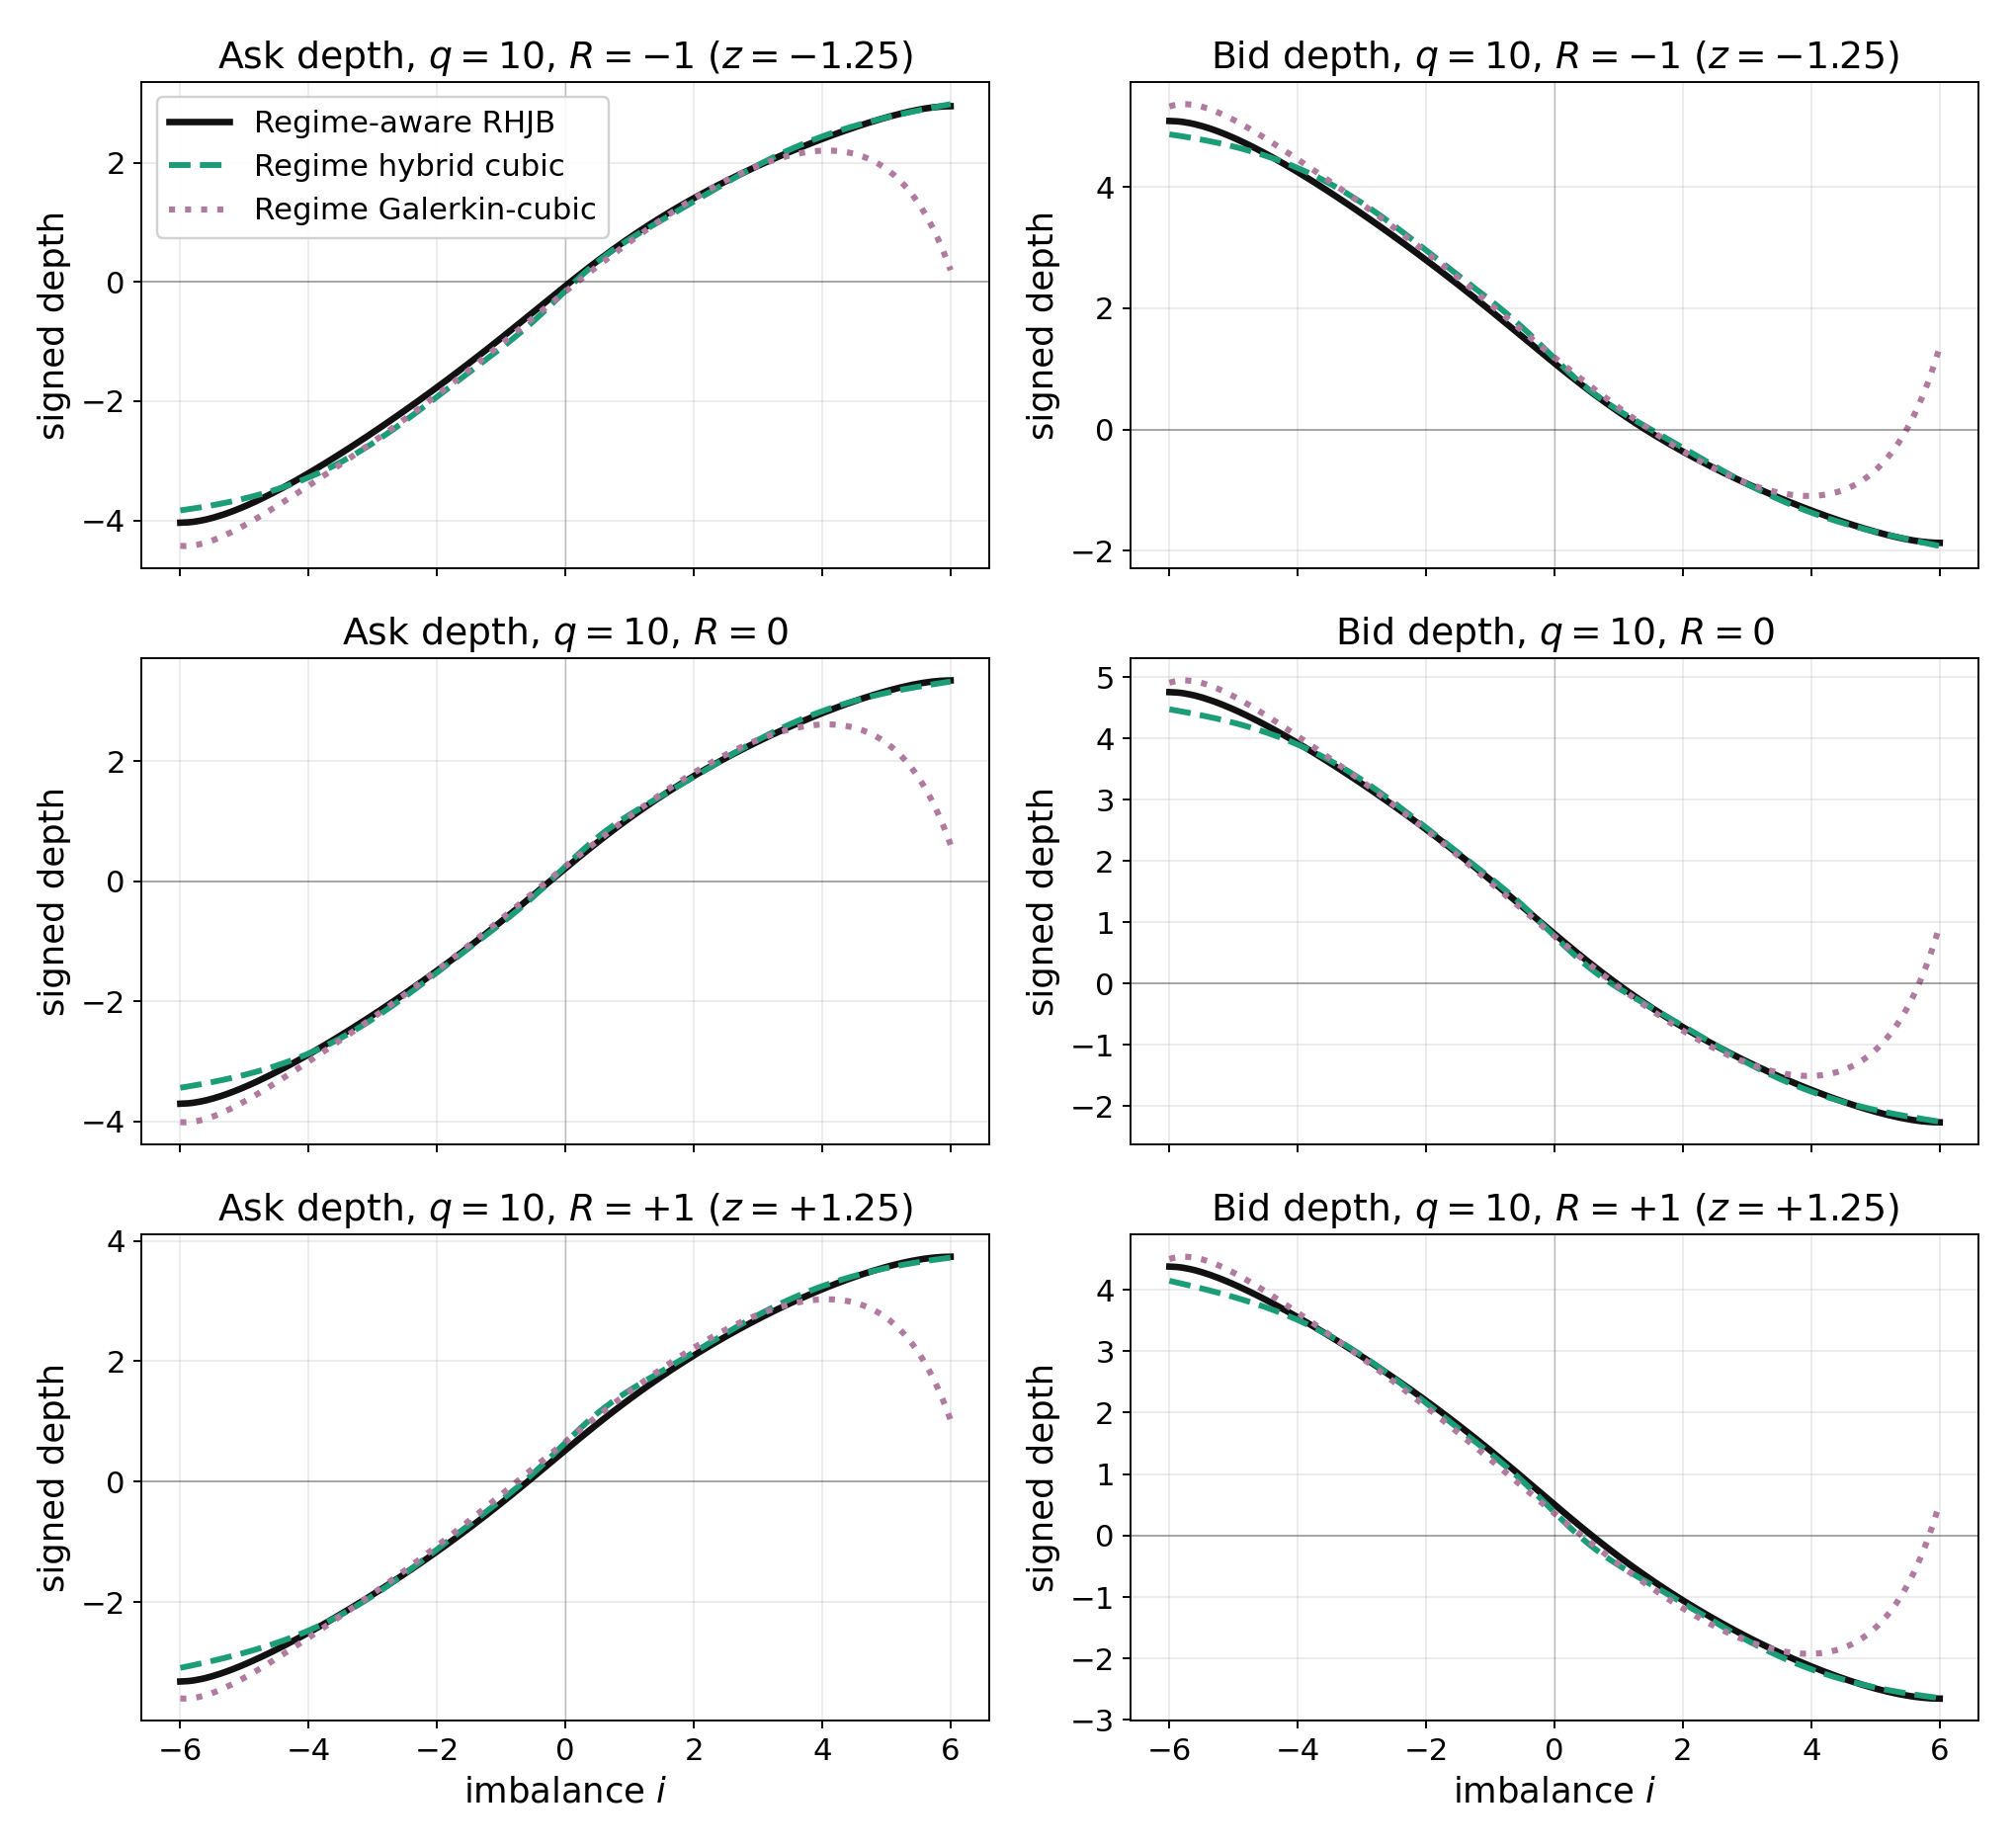
\includegraphics[width=0.85\linewidth]{regime_fast_alpha_depths_vs_i_v2.png}
\caption{Regime depths vs imbalance \(i\) (rows: the three regimes) at \(q=10\).
Numerical regime RHJB (solid) overlaid with the body hybrid flow-gated cubic
\eqref{eq:regime_sccubic_quotes} (dashed) and the appendix Galerkin-cubic
\eqref{eq:regime_galerkin_quotes} (dotted).  The hybrid cubic tracks the
RHJB across all three regimes; the single-loading Galerkin form deviates sharply in the
tails.  Pooled ask\(+\)bid depth RMSE vs the RHJB (over \(q\in\{-5,0,10,15\}\) and the three regimes): hybrid cubic
\(\approx0.10\), Galerkin \(\approx0.65\), affine \eqref{eq:regime_ansatz_quotes_qYr}
\(\approx0.52\).}
\label{fig:regime_depths_vs_i}
\end{figure}


\begin{figure}[htbp]
\centering
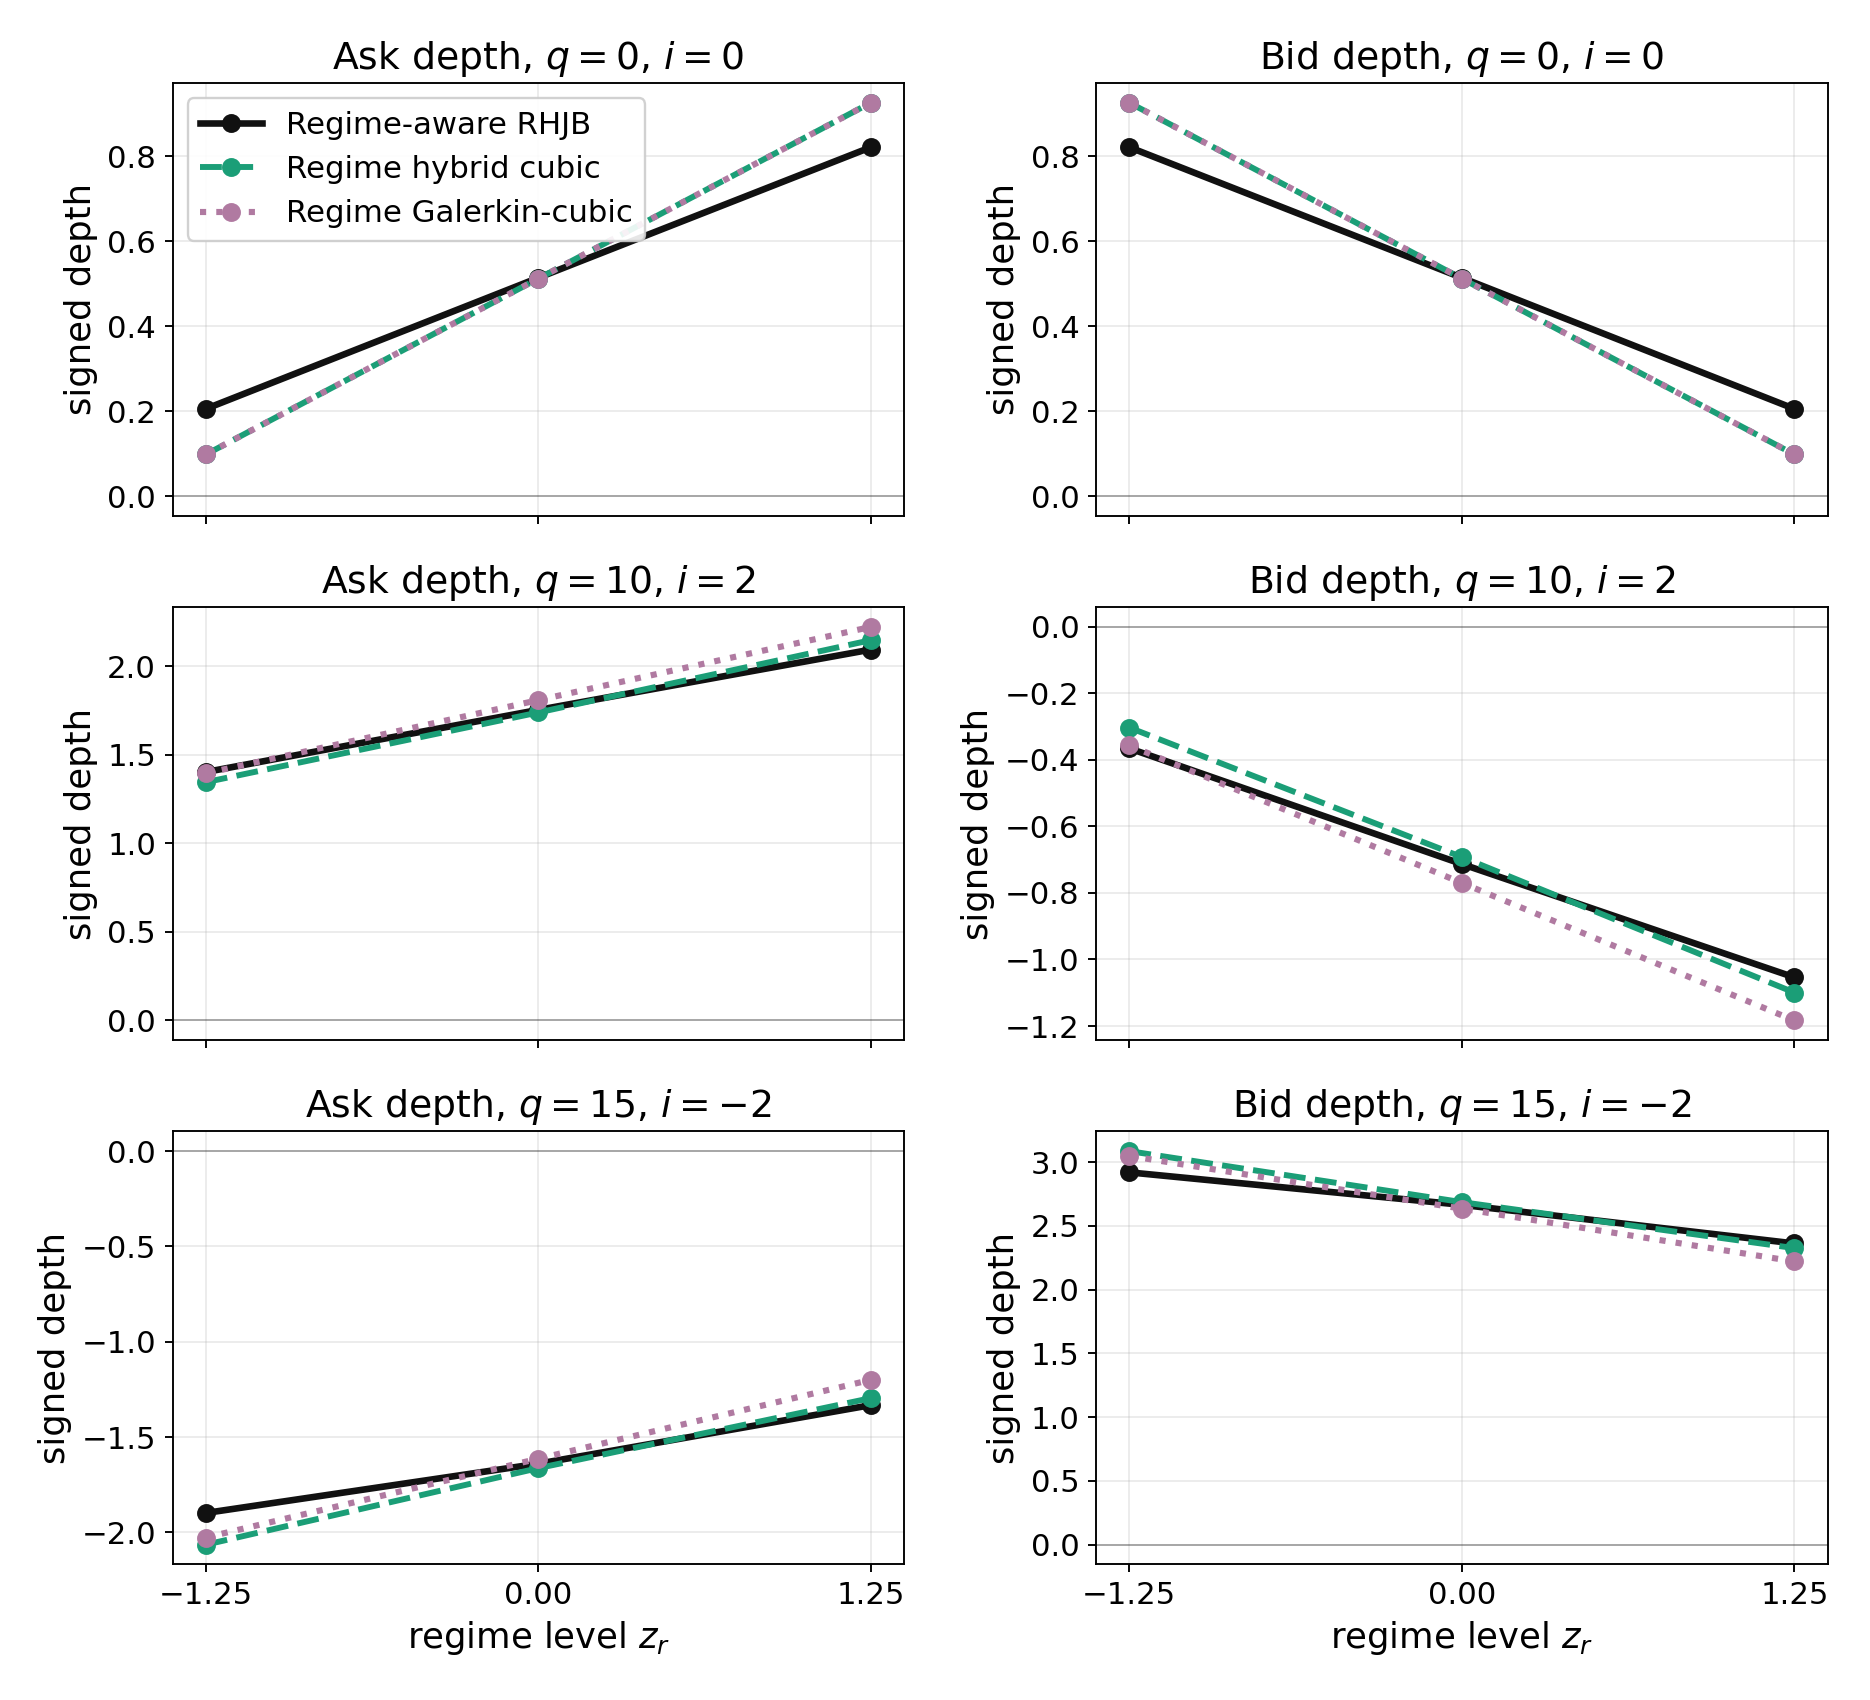
\includegraphics[width=0.75\linewidth]{regime_fast_alpha_depths_vs_z_v2.png}
\caption{Regime depths as a function of the regime level
\(z_r\in\{-1.25,0,+1.25\}\) at selected \((q,i)\): numerical regime RHJB (solid)
against the hybrid cubic (dashed) and the Galerkin-cubic (dotted).  Both closed
forms carry the ungated channel \(A_Rz_r\) with \(A_R\approx0.331\); at
balanced flow (\(q=0\), \(i=0\)) the RHJB's own slope in \(z_r\) is \(0.246\),
close to the Galerkin-local value \(B_G\approx0.257\) of
Appendix~\ref{app:regime_refined}, so the imported \(A_R\) overstates the regime
response at the origin by about a third; away from the origin the hybrid
cubic, whose cubic skew also reads the regime through \(\vartheta_{\rm full}\),
stays closer to the RHJB.}
\label{fig:regime_depths_vs_alpha_z}
\end{figure}

\begin{remark}[Domain convergence of the depth RMSE]
\label{rem:domain_convergence}
The depth RMSEs above are computed on the \([-6,6]\) solve grid.  The
\emph{uniform} RMSE over that band is sensitive to the truncation of the solve
domain (the truncated \([-6,6]\) solve understates the tail error), whereas the
RMSE weighted by where the process lives is stable.  Re-solving on \([-9,9]\) at the same \(\Delta i=0.1\) and re-evaluating
on the common interior \(|i|\le6\) (pooled over \(q\in\{-5,0,10,15\}\) and, for the
regime, the three regimes; entries recomputed on a common \(241\)-point band, so
they may differ from the body's figures in the last digit):
\[
\begin{array}{l|ccc|ccc}
& \multicolumn{3}{c|}{\text{uniform}} & \multicolumn{3}{c}{\text{stationary-weighted}}\\
\text{solve domain} & \text{toy} & \text{fast-}\alpha & \text{regime} & \text{toy} & \text{fast-}\alpha & \text{regime}\\\hline
{[-6,6]} & 0.052 & 0.097 & 0.103 & 0.031 & 0.049 & 0.086\\
{[-9,9]} & 0.066 & 0.169 & 0.164 & 0.032 & 0.058 & 0.092
\end{array}
\]
The toy and fast-alpha weights are the centred OU law \(\mathcal N(0,\eta^2/2\beta)\); the regime
weight is the joint invariant density \(p_r(i)\) of \((I,R)\), whose per-regime
means are shifted to \(\pm0.75\) rather than centred.  The uniform figure grows by
\(28\%\) (toy), \(75\%\) (fast-alpha) and \(60\%\) (regime) on the wider grid while the
stationary-weighted figure barely moves: the closed forms are robust over the
visited \((I,R)\) states, and the uniform RMSE---dominated by the sparsely visited
tails---overstates the typical error.
\end{remark}

\begin{remark}[Calibration-local fidelity]
\label{rem:calibration_local}
The depth accuracy just reported is local to the baseline calibration, not a
uniform parameter-robustness claim.  In a frozen holdout campaign, the current
hybrid flow-gated cubic had invariant-weighted relative depth RMSE (absolute
depth RMSE divided by the RHJB depth RMS) of \(3.46\%\) at the fast-alpha
baseline and \(5.11\%\) at the regime baseline.  Representative stresses were
much harder: across seven wide-imbalance and wide-flow corners the relative
error ranged from \(43\%\) to \(357\%\), the extremes being
\((\beta,\eta)=(0.00625,0.64)\) for fast-alpha and \(\eta=0.64\) for the
regime.  All corresponding RHJB solves converged,
and expanded-domain checks ruled out truncation as the explanation in the
wide-imbalance corners.  A predeclared deterministic promotion gate therefore
failed, so no stressed Monte Carlo comparison was run.  The economic Monte
Carlo conclusions below should consequently be read as baseline-calibration
evidence; the elementary formulas should be revalidated after material
parameter changes.
\end{remark}

\begin{table}[htbp]
\centering
\setlength{\tabcolsep}{4pt}
\begin{tabular}{lrrrrrr}
\toprule
Policy & Total & Penalized & Spread & Alpha drift & \(\E|Q_t|\) & \(Q^{\rm life}_{.01},Q^{\rm life}_{.99}\)\\
\midrule
GLFT & \(-2383.76\) & \(-4153.82\) & \(2337.70\) & \(-4720.89\) & \(16.48\) & \([-41,41]\)\\
\(I\)-aware & \(492.20\) & \(281.23\) & \(2028.94\) & \(-1537.54\) & \(5.72\) & \([-14,14]\)\\
Alpha/\(I\)-aware & \(2578.30\) & \(2248.43\) & \(568.18\) & \(2009.74\) & \(7.40\) & \([-16,16]\)\\
Regime-aware & \(3001.21\) & \(2423.51\) & \(556.21\) & \(2445.76\) & \(9.68\) & \([-21,21]\)\\
Regime hybrid cubic & \(3099.86\) & \(2400.31\) & \(483.28\) & \(2616.99\) & \(10.81\) & \([-22,22]\)\\
Regime Galerkin-cubic & \(2999.12\) & \(2283.20\) & \(493.77\) & \(2505.79\) & \(10.84\) & \([-24,24]\)\\
\bottomrule
\end{tabular}
\caption{Regime Monte Carlo summary at the parameters of
Table~\ref{tab:parameters}; columns as in Table~\ref{tab:alpha_summary}.  All
policies stay far from the \([-60,60]\) inventory boundary.}
\label{tab:regime_summary}
\end{table}

\begin{figure}[htbp]
\centering
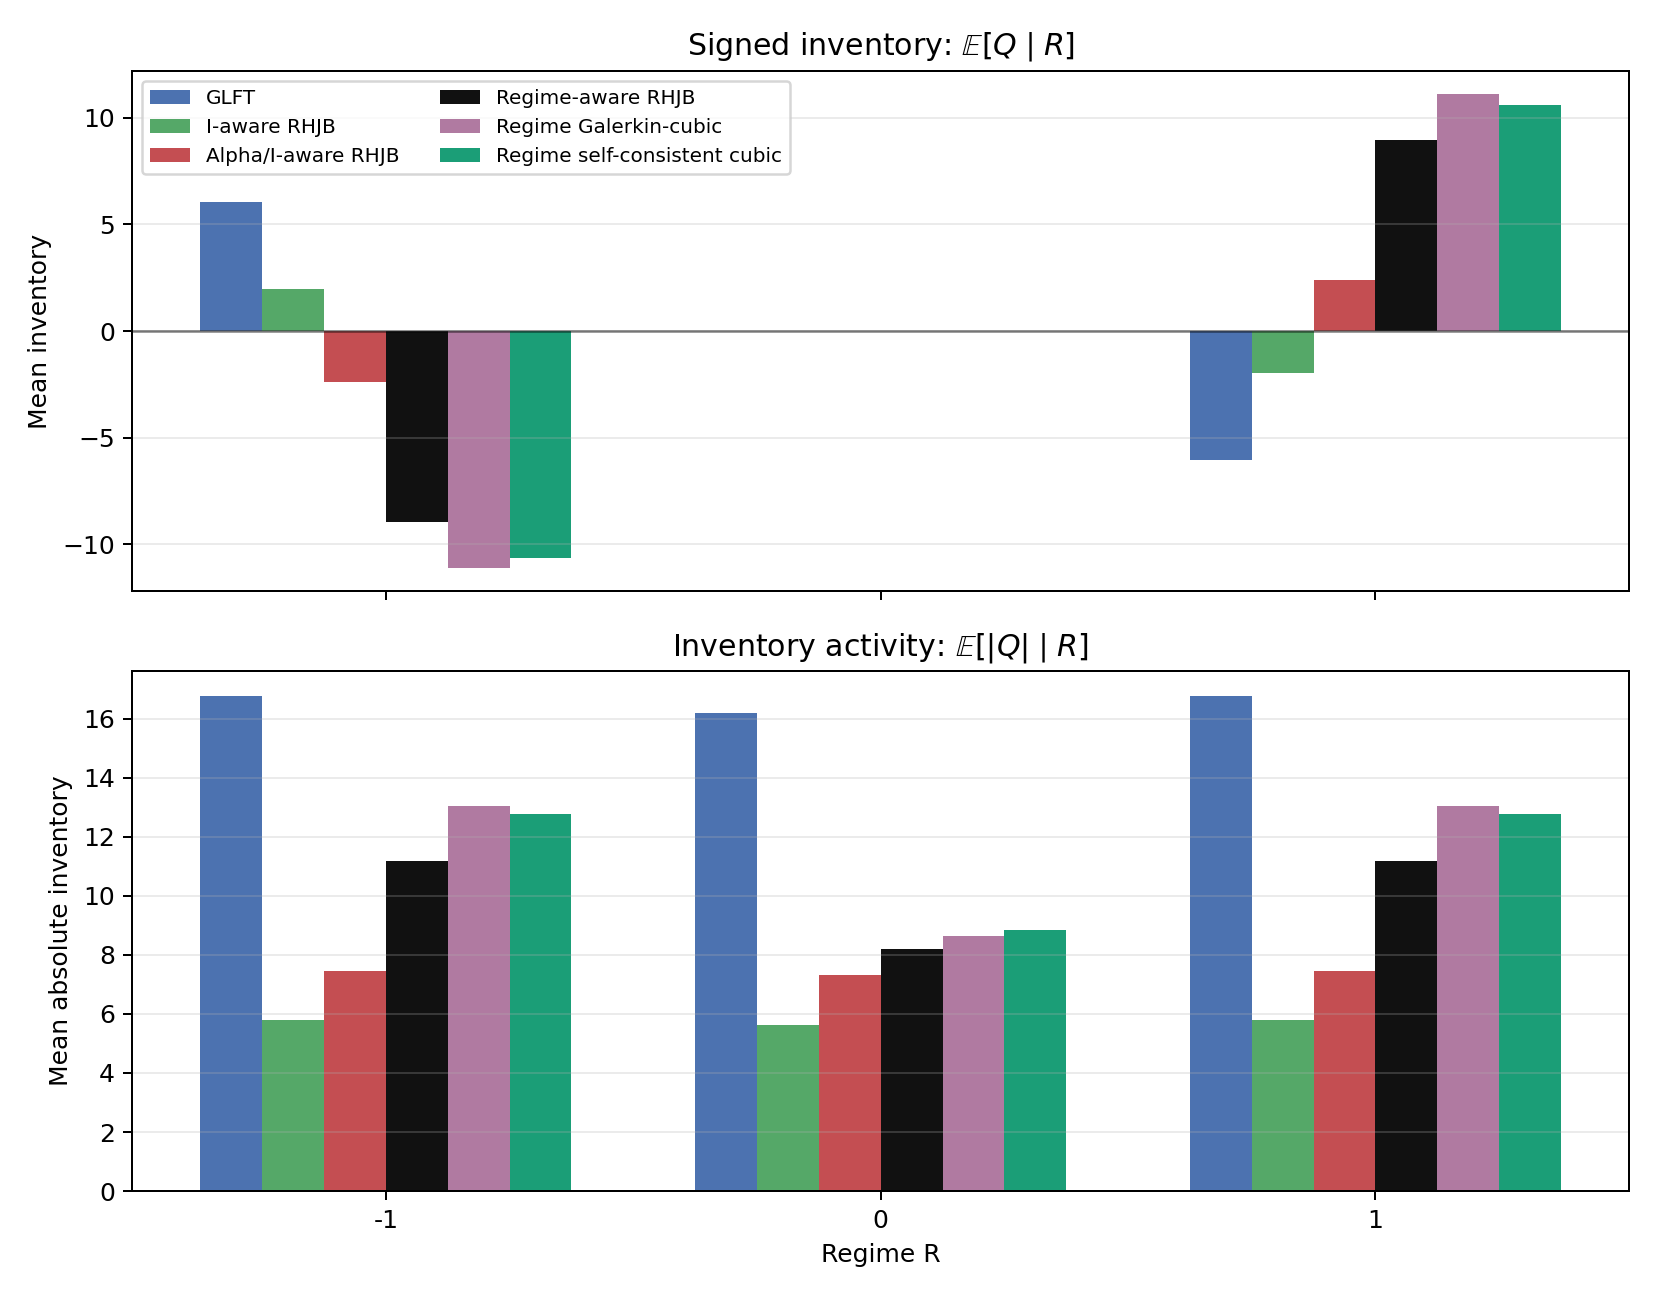
\includegraphics[width=0.78\linewidth]{regime_fast_alpha_inventory_by_regime.png}
\caption{Regime study: mean signed inventory by slow regime,
\(\E[Q_t\mid R_t]\), pooled over paths and times.  In the neutral regime the
means of all six policies vanish by symmetry (each within \(0.02\) units), so
no bar is visible at \(R=0\); the persistent-pressure regimes are discussed
in the text.}
\label{fig:regime_inventory_by_regime}
\end{figure}

\begin{figure}[htbp]
\centering
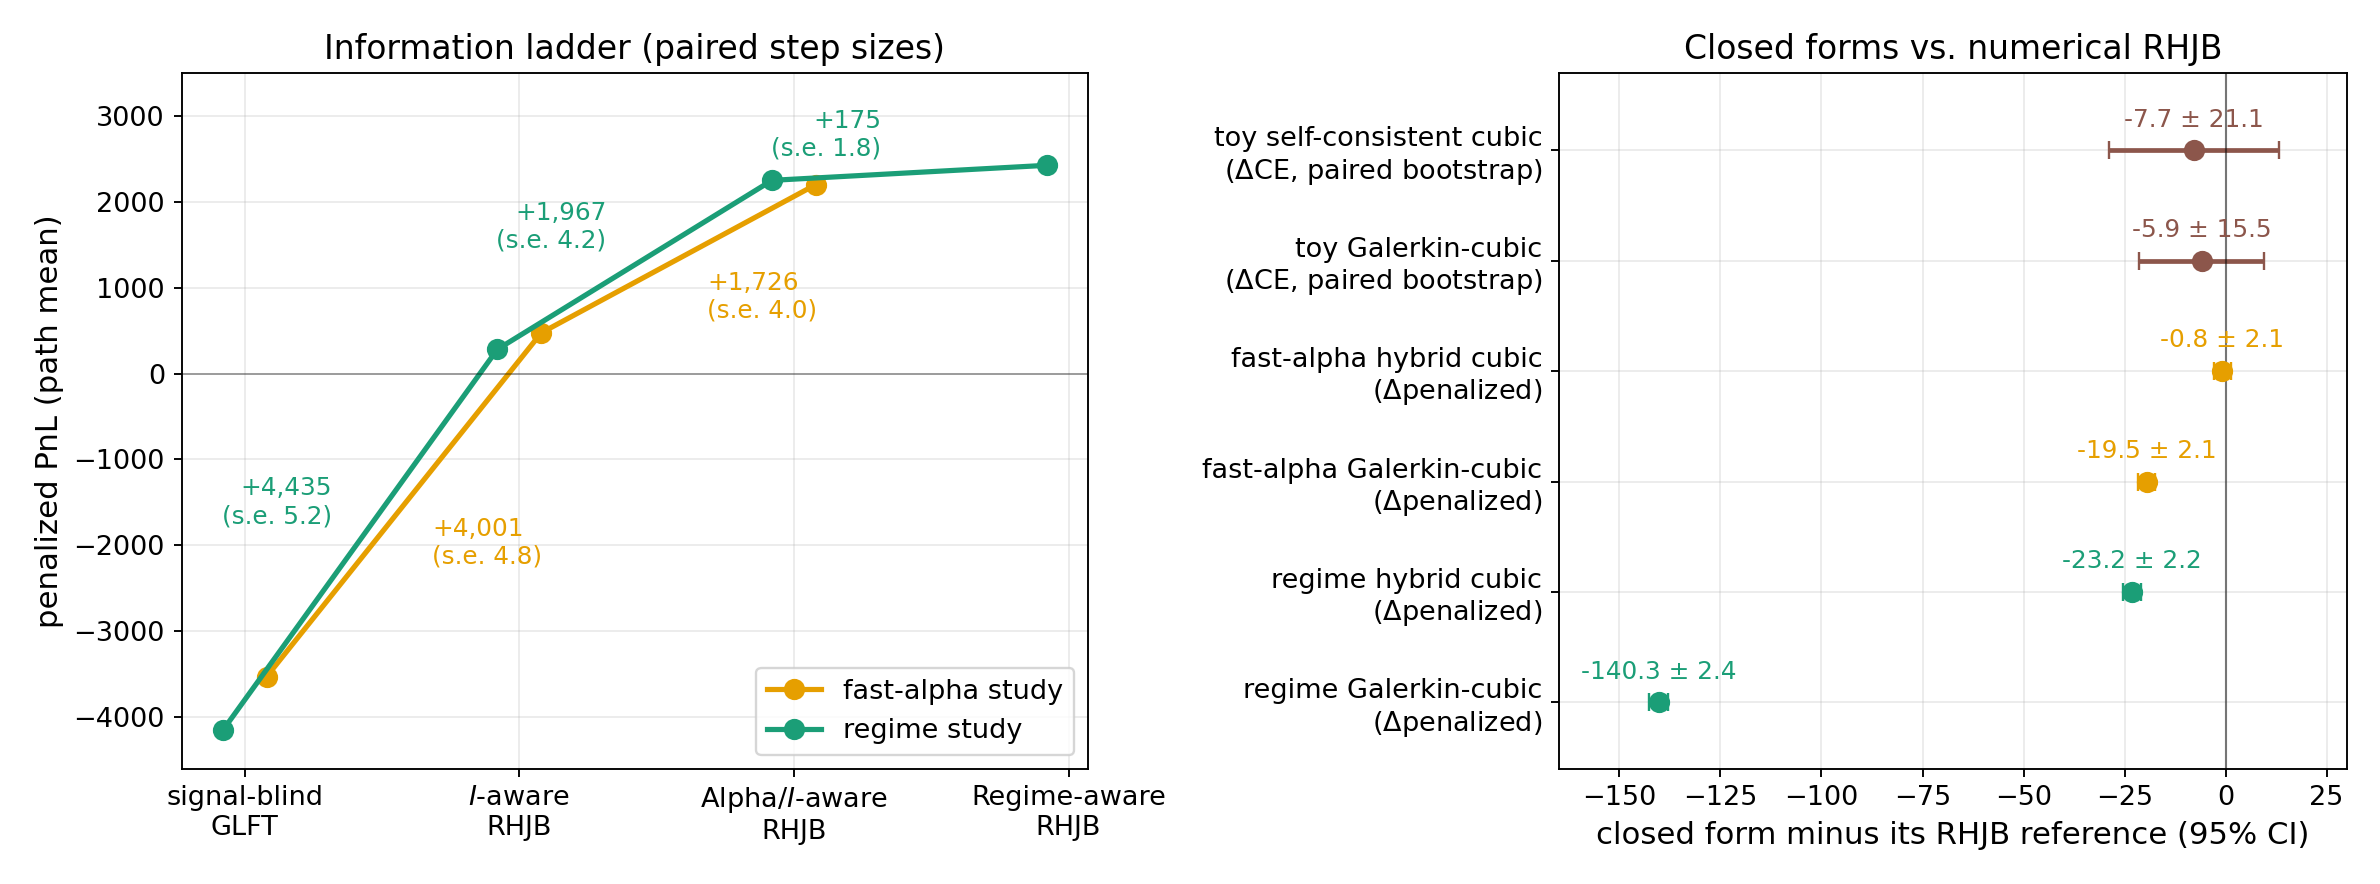
\includegraphics[width=0.9\linewidth]{paired_ladder.png}
\caption{Paired contrasts across the three studies.  Left: penalized-PnL
levels of the RHJB ladder in the fast-alpha (Table~\ref{tab:alpha_summary})
and regime (Table~\ref{tab:regime_summary}) studies, each step annotated with
its paired difference and standard error on the shared environment paths.
Right: each closed form against its own RHJB reference---toy:
paired-bootstrap \(\Delta\mathrm{CE}\) against the \(I\)-aware RHJB
(\(2000\) path resamples; exponential-weight ESS \(73\) and \(145\));
fast-alpha: \(\Delta\)penalized PnL against the Alpha/\(I\)-aware RHJB;
regime: \(\Delta\)penalized PnL against the regime-aware RHJB, point
estimates from Table~\ref{tab:regime_summary} without paired standard errors
(open markers).  Bars are \(95\%\) intervals.}
\label{fig:paired_ladder}
\end{figure}

Because all six policies run on the \emph{same} exogenous
\((S,I,R,\alpha)\)-environment, the table is a ladder in penalized PnL as
information is added: signal-blind GLFT (\(-4154\)) is severely adversely
aligned with alpha; observing \(I\) lifts it to \(+281\) (\(+4435\), by far the
largest step), the fast-alpha channel to \(+2248\) (a \(+1967\) step), and the
regime-aware policy to \(+2424\).  Over the alpha/\(I\)-aware benchmark,
\[
\Delta_R=\mathrm{Penalized}_{\alpha/I/R}-\mathrm{Penalized}_{\alpha/I}
\approx+175.1
\quad(\text{paired s.e.}\ 1.8,\ \ 95\%\ \text{CI}\ [171.5,\,178.6])
\]
is statistically clear but small: about \(8\%\) on top of the alpha/\(I\)-aware
level, against \(+4435.0\) (paired s.e.\ \(5.2\)) from observing flow and
\(+1967.2\) (paired s.e.\ \(4.2\)) from using alpha; contrasts are paired on the
shared paths (paired correlation \(0.77\) for \(\Delta_R\), roughly halving the
unpaired s.e.\ \(\approx3.5\)).  We do not read \(\Delta_R\) as the \emph{pure}
value of observing \(R\): the benchmark is solved under a centred, no-regime OU,
so \(\Delta_R\) also reflects correcting the imbalance dynamics to the switching
generator (a pure regime value needs a regime-blind policy optimised under the
switching dynamics).  \(R_t\) helps because it carries information about the
\emph{future} path of \(I_t\)---\(\mathcal{L}_{I,R}\) propagates values across
likely future \((I,R)\)-states and the loading adds the persistent-regime term
\(A_R z_r\) (\eqref{eq:regime_closed_loading}, \eqref{eq:regime_sc_shift})---but
only as a modest refinement.  Figure~\ref{fig:regime_inventory_by_regime} shows
mean signed inventory by regime: the regime-aware RHJB and both closed forms
lean about ten units into the persistent-pressure regimes, the Alpha/\(I\)-aware
policy about two, and signal-blind GLFT and the \(I\)-aware policy hold
inventory of the wrong sign there.  Both closed forms fall short of the regime-aware RHJB in penalized PnL---the
body hybrid flow-gated cubic by about \(23\) (\(\approx1\%\), penalized
\(\approx2400\)), the offline Galerkin-cubic by about \(140\)
(\(\approx2283\)), the ordering of the depth figures.  Paired standard errors
were not computed for these two contrasts, so we report them as point
differences; for scale, the corresponding fast-alpha contrasts have paired
standard errors near \(1.1\).  Both forms quote more aggressively into the
regime signal (\(\E|Q_t|\approx10.8\) versus \(9.7\)), earning more raw PnL
and paying for it in inventory penalty.  Figure~\ref{fig:paired_ladder}
collects the paired contrasts of the three studies.




\FloatBarrier

\section{Numerical Implementation}
\label{sec:numerical_implementation}

The parameters and policies of the three studies are collected in
Tables~\ref{tab:parameters} and~\ref{tab:policies} (Section~\ref{sec:toy});
this section records how the profiles and simulations were computed.

\subsection{Stationary Profiles}

The stationary quoting profiles of Sections~\ref{sec:toy}--\ref{sec:regime}
are obtained by advancing the split scheme of Section~\ref{subsec:strang} in
pseudo-time while repeatedly removing a common additive level---the nonlinear
analogue of the power method for the principal eigenvector, which is what the
profile literally is in the GLFT case.  The step is \(\Delta\tau=0.25\)
(\(0.5\) for the toy); every \(20\) steps the full recovered ask and bid depth
arrays are compared with those of the preceding check, and the iteration stops
when the maximum absolute change falls below \(2\times10^{-8}\), reached by
\(\tau\approx810\)--\(1085\) in all runs.  The exact finite-grid GLFT benchmark
is its principal eigenvector and the Gaussian GLFT baseline is analytic;
neither uses this iteration.  The subsequent Monte Carlo simulations use the
seeds \(20260519\) (toy, with seed\(+777\) for its independent shared
environment), \(86420\) (fast-alpha) and \(24680\) (regime).

\subsection{Finite Grids}

All PDE computations use the inventory grid \(\Qcal\) with \(q_{\max}=60\),
the boundary rule of Section~\ref{sec:setup} (the unavailable depth may be
viewed as \(+\infty\)), and the \(J=121\)-point imbalance grid
\(i_j=-6+0.1j\), \(j=0,\ldots,J-1\), on which the OU generator is discretized
by the centered differences and ghost-node edge closure of
Section~\ref{subsubsec:toy_signal_step}---a numerical device for the truncated
domain, not an economic assumption about the unbounded OU process.

\paragraph{Depth harness.}
Every depth RMSE quoted in the paper is the root mean square of
\(\delta_{\rm closed\ form}-\delta_{\rm RHJB}\) over the pooled ask and bid
depths.  Along the imbalance axis the mean is uniform over a \(301\)-point
evaluation grid on \([-6,6]\) (\(\Delta i=0.04\); the RHJB depths are
interpolated from the \(J=121\)-point solve grid), or weighted by the
stationary law where stated, and pooled over
\(q\in\{-5,0,10,15\}\) and, in the regime model, the three regimes; along the
inventory axis it is taken over the inventory window and imbalance slices of
the corresponding depth figure.  Appendix~\ref{app:toy_refined} pools its
imbalance-axis figures over \(q\in\{0,3,5\}\) and its inventory-axis figures
over \(|q|\le14\).

\subsection{Simulation Protocol}

All reported Monte Carlo runs start from \(S_0=0\), \(Q_0=0\), with
\(I_0=0\) in the toy and fast-alpha experiments and \(\alpha_0=0\) in the
fast-alpha and regime experiments.  The regime experiment uses a
\emph{quasi-stationary frozen-regime} initialization:
\(R_0\sim(\tfrac14,\tfrac12,\tfrac14)\) over the three regimes and, given
\(R_0\), \(I_0\sim\mathcal N(z_{R_0},\eta^2/2\beta)\).  This is not the exact
joint invariant law of \((I,R)\), whose conditional means are \(\pm0.75\)
rather than \(z_{\pm1}\) (Remark~\ref{rem:domain_convergence}); over
\(T=10000\) the initialization bias relaxes on the \(1/\beta\) timescale.

Within each step, quotes and intensities use the left-endpoint state.  \(S\),
\(I\), and the diffusive part of \(\alpha\) are advanced by Euler--Maruyama;
maker fills and aggregate market-order counts are Poisson increments with
left-endpoint means.  The regime chain uses a one-jump-per-step update with
holding probability \(\e^{-\Delta t/\tau_R}\) and jump destinations read from
\(\Gamma\), not the exact matrix exponential.

The numerical RHJB policy is computed on the finite \(I\)-grid and evaluated by
linear interpolation in \(i\); if the OU state leaves \([-6,6]\), the lookup
clips \(I_t\) to the nearest boundary point before interpolation, while
\(I_t\) itself is not reflected.  The fast-alpha and regime Galerkin forms
use the same \(i_c=\operatorname{clip}(I_t,-6,6)\), since their single global
loading otherwise drives the curvature off-grid
(Remark~\ref{rem:regime_galerkin}); the body cubic closures and the toy
Galerkin form use the true \(I_t\).  The shares of recorded time--path
states outside the solve grid are \(0.298\%\) (toy), \(0.302\%\)
(fast-alpha) and \(0.490\%\) (regime); no clipping ablation was run, so the
closed-form-versus-RHJB contrasts differ in the off-grid rule as well as in
the quoting formula.

Each maker side is simulated as a Poisson increment
\(\Delta N_t^\ell\sim\operatorname{Poisson}(\Lambda_t^{\ell,0}
\e^{-k\delta_t^\ell}\Delta t)\), with quotes held fixed within the step; a
count that would move inventory outside \(\Qcal\) is truncated at the remaining
inventory capacity on that side.  The simulation is thus a finite-grid
approximation of the continuous-time intensity model that allows multiple
fills per side per step.  The aggregate counts \(M^\ell\) driving \(\alpha_t\)
are also Poisson increments with means \(\Lambda^{\ell,0}(I_t)\Delta t\),
sampled, conditional on the left-endpoint state and quotes, independently of
the maker-fill counts, consistently with the reduced-form assumption of
Section~\ref{sec:fast_alpha}.

\subsection{Splitting Scheme}

All three models advance by the Strang split of Section~\ref{subsec:strang};
only the operators change: \(\mathsf A_{i_j}^{\rm toy}\) of \eqref{eq:toy_w}
in the toy model and \(\mathsf A_{i_j}^{\alpha}\) of \eqref{eq:fast_alpha_w}
in the fast-alpha and regime models (at each \((i_j,r)\) in the latter), and,
in the regime model, \(\mathsf L_{I,R}^\Delta\) discretizing the joint
generator \eqref{eq:regime_joint_generator} in place of
\(\mathsf L_I^\Delta\).  The split keeps both blocks linear: a global
Cole--Hopf change would make \(\Lcal_I(k^{-1}\log w_q)\) nonlinear.  After
each full step \(v_0(0)\) (its neutral-regime counterpart in the regime model)
is subtracted from the relative value, leaving the quotes unchanged.

\subsection{PnL Decomposition}

In the fast-alpha and regime simulations, the mark-to-market wealth satisfies
\[
\dd(X_t+Q_tS_t)
=
\delta_t^a\,\dd N_t^a
+\delta_t^b\,\dd N_t^b
+Q_t\,\dd S_t.
\]
Since
\[
\dd S_t=\alpha_t\,\dd t+\sigma\,\dd W^S_t,
\]
the pathwise decomposition is
\begin{equation}
\PnL_T
=
\int_0^T\delta_t^a\,\dd N_t^a
+\int_0^T\delta_t^b\,\dd N_t^b
+\int_0^T Q_t\alpha_t\,\dd t
+\int_0^T Q_t\sigma\,\dd W^S_t.
\label{eq:pnl_decomposition}
\end{equation}
The last term is a zero-mean martingale that contributes to realized PnL
dispersion but not to its mean; the tables report the full realized PnL
(``Total'') together with the spread and \emph{alpha-drift} components, the
latter positive when the policy is, on average, long when \(\alpha_t>0\) and
short when \(\alpha_t<0\).

The penalized PnL reported in the fast-alpha and regime tables is the
diagnostic
\begin{equation}
\PnL_T^{\rm pen}
=
\PnL_T
-\frac{\gamma\sigma^2}{2}\int_0^T Q_t^2\,\dd t
-c_T Q_T^2,
\qquad
c_T=0.01.
\label{eq:penalized_pnl_diagnostic}
\end{equation}
The penalty uses the RHJB's own running inventory-risk scale
\(\gamma\sigma^2/2\); the penalized quantity is a post-simulation diagnostic,
not the objective used to compute the policies (Remark~\ref{rem:xi}); the
terminal term \(c_TQ_T^2\) is a small liquidation charge (at most
\(c_Tq_{\max}^2=36\) against penalized PnLs in the thousands) that
discourages end-of-horizon inventory.

\begin{remark}[The two objectives as a single $\xi$-family]
\label{rem:xi}
Up to its terminal term, the diagnostic \eqref{eq:penalized_pnl_diagnostic} is
the running-penalty objective
\(\E\bigl[\PnL_T-\tfrac12\gamma\sigma^2\int_0^TQ_t^2\,\dd t\bigr]\) of
\cite{CarteaJaimungalPenalva2015}, while the policies derive from the CARA
terminal utility~\eqref{eq:as_objective} (up to the simplification of
Definition~\ref{def:srn_rhjb} when state-dependent).  In the \(\xi\ge0\)
family of reduced HJBs of \cite{Gueant2017}, CARA is \(\xi=\gamma\) and the
running-penalty model \(\xi=0\), with the same \(\tfrac12\gamma\sigma^2q^2\)
inventory term; \(\xi\) is the aversion to non-execution risk, \(\gamma\) to
price risk.  The diagnostic thus scores CARA-derived policies under
\(\xi=0\), isolating realized inventory risk from non-execution-risk aversion.
\end{remark}

\section{Conclusion}
\label{sec:conclusion}

The GLFT benchmark supplies the inventory curvature and the signal-blind
baseline; the three extensions modulate it with order-flow information through
one optimal-quote map.  Persistent flow imbalance matters even without
predictive drift, because it changes future fill composition, and the
\(I\)-dependent skew controls inventory far more tightly than GLFT; the
fast-alpha drift reward \(q\alphabar(i)\) (Approximation~\ref{prop:alpha_bar})
turns the observable imbalance into positive alpha-drift PnL, reversing the
adverse alignment of the signal-blind maker; and the slow regime, acting only
through the conditional future law of \(I_t\), leaves the Cole--Hopf inventory
block intact at fixed \((i,r)\) and adds one persistent-regime term, with the
regime-aware RHJB attaining the best penalized performance.

Four simplifications bound what the results establish.  The state-dependent
policies solve the signal-risk-neutral RHJB (Definition~\ref{def:srn_rhjb}),
whose depth gap to the exact CARA solution is small in the toy model but
comparable to the closed-form error in the fast-alpha model
(Remark~\ref{rem:srn_size}); the stationary profiles assume the ergodic limit
of Remark~\ref{rem:ergodic_existence}, which we do not prove; alpha enters
through the frozen-\(I\) mean \(\alphabar(I)\), whose origin slope \(0.036\)
exceeds that of the exact conditional mean by about \(30\%\)
(Remark~\ref{rem:frozen_i_robustness});
and the regime-aware policy observes \(R_t\) perfectly, so its performance is
a full-information ceiling rather than what a filtered regime would deliver.
The signal-blind benchmark is the textbook GLFT rule at the maker's own
\((\gamma,\sigma)\), not the optimal policy of a maker who knows the model but
does not observe \(I_t\).  Under the CARA certainty equivalent of the toy study
that gap does bound the value of flow information from above, GLFT being
admissible in the signal-blind class; under the penalized diagnostic it does
not, since a signal-blind maker that merely rescales its inventory-risk
parameter erases the first ladder step
(Remark~\ref{rem:blind_recalibration}).  Natural next steps are a filtered-regime policy, an
empirical calibration of the imbalance process to trade-sign
autocorrelations, and a closure that remains accurate in the wide-imbalance
corners of Remark~\ref{rem:calibration_local}.

All numerical statements concern the baseline calibration and the reported
finite-grid, time-discretized experiments.  The frozen holdouts of
Remark~\ref{rem:calibration_local} show that the elementary closures can
deteriorate materially under wide-imbalance stresses: they are interpretable
calibration-local approximations, not uniformly accurate policies over the
parameter space.

\appendix

\section{Global Galerkin toy loading}
\label{app:toy_refined}

The body's self-consistent cubic closed form \eqref{eq:toy_curvature_quotes}---with the
dynamic curvature \(r(i)\) of \eqref{eq:toy_dynamic_r_main} and the
side-asymmetric cubic \(s(i)\) of \eqref{eq:toy_curvature_rs}---already tracks
the numerical RHJB closely off balanced flow with an elementary loading and no
fitted constants.  This appendix records one further, \emph{global} saturating
refinement whose amplitude and inner scale are fixed by an offline OU-Gaussian
moment projection (the Galerkin pair \((A,\varrho)\)), carried through those
same curvature and cubic closures.  On the depth harness evaluated at
\(q\in\{0,3,5\}\), it tightens the imbalance-axis fit (pooled depth RMSE
\(0.057\to0.030\)) at the cost of the inventory axis (\(0.030\to0.049\) on
\(|q|\le14\)) and, unlike the body form, requires an offline numerical moment
solve.

\begin{approximation}[Global Galerkin loading]
\label{prop:toy_galerkin}
Restoring the \(i\)-dependent curvature \(r(i)\) of
\eqref{eq:toy_dynamic_r_main} and the execution factor
\(\e^{-r(i)/2}=1+O(r_{\rm G})\) in the \(q^1\) source, under the
small-curvature truncation of the proof of
Approximation~\ref{prop:toy_curvature}, gives the retained-order residual
\begin{equation}
\mathcal R_1(i):=\frac{\eta^2}{2}h_I''-\beta i\,h_I'
+\frac{2\kappa}{k}\,\frac{\sinh\vartheta}{\sqrt{\cosh i\,\cosh\vartheta}}\,
\e^{-r(i)/2}=0 ,\qquad
\vartheta=i-kh_I,\ \ r(i)=r_{\rm G}\sqrt{\tfrac{\cosh i}{\cosh\vartheta}} .
\label{eq:toy_loading_ode}
\end{equation}
Differentiating the untruncated cubic execution sum at \(q=0\) replaces
\(r\sinh\vartheta\) by \(s\cosh(\vartheta-s/3)+r\sinh(\vartheta-s/3)\), an
omitted source that is formally \(O(c_{\rm GLFT}r_{\rm G}^2/k)\) at fixed or
moderate imbalance since \(s=O(r_{\rm G}^2)\); \(\mathcal R_1\) is thus the
\(q^1\) residual through \(O(r_{\rm G})\), not the full cubic-RHJB
coefficient.  The curvature ratio \(\sqrt{\cosh i/\cosh\vartheta}\) equals
one at \(i=0\) (retained execution factor \(\e^{-r_{\rm G}/2}\approx0.974\))
and grows only at moderate \(|i|\), which a Taylor expansion about the
origin such as the leading-order loading \eqref{eq:toy_loading_ansatz}
misses: the effect lives at the moderate \(|i|\) the imbalance actually
visits.  We therefore impose \eqref{eq:toy_loading_ode} \emph{on average}
over the band the imbalance populates, with no fit to RHJB data, taking for
\(A\in\R\), \(\varrho>0\) the saturating trial loading
\begin{equation}
h_G(i)=A\,\frac{i}{\sqrt{1+\dfrac{\beta}{\varrho\,\eta^2}\,i^2}},
\label{eq:toy_galerkin_loading}
\end{equation}
written \(h_G\) throughout the appendices to distinguish this globally
projected family from the body's elementary loading \(h_I\) of
\eqref{eq:toy_loading_ansatz}, and fixing \((A,\varrho)\) by Galerkin
projection of \(\mathcal R_1\) onto \(\{i,i^3\}\) under the OU stationary
weight \(\omega_{\rm OU}(i)=\e^{-\beta i^2/\eta^2}\),
\begin{equation}
\int_{\R} \mathcal R_1(i)\,i\,\omega_{\rm OU}(i)\,\dd i=0,\qquad
\int_{\R} \mathcal R_1(i)\,i^3\,\omega_{\rm OU}(i)\,\dd i=0 .
\label{eq:toy_galerkin_moments}
\end{equation}
The loading \eqref{eq:toy_loading_ansatz} is not in this family but shares
the \(\varrho=1\) saturation scale \(\eta/\sqrt\beta\), fixing its amplitude
pointwise at \(i=0\) instead; the optimal-quote map
\eqref{eq:state_dep_recovery} then returns the Galerkin closed-form quotes
\begin{align}
\delta_{\rm galerkin}^a(q,i)&=\delta_\gamma+h_G(i)-\frac{r(i)}{2k}(2q-1)
+\frac{s(i)}{k}\Bigl(q^2-q+\tfrac13\Bigr),\notag\\
\delta_{\rm galerkin}^b(q,i)&=\delta_\gamma-h_G(i)+\frac{r(i)}{2k}(2q+1)
-\frac{s(i)}{k}\Bigl(q^2+q+\tfrac13\Bigr),\label{eq:toy_galerkin_quotes}
\end{align}
with \(h_G\) of \eqref{eq:toy_galerkin_loading}, effective imbalance
\(\vartheta(i)=i-kh_G(i)\), \(r(i)\) of \eqref{eq:toy_dynamic_r_main},
\(s(i)\) of \eqref{eq:toy_curvature_rs}, and \((A,\varrho)\) solving the
Gaussian-moment system \eqref{eq:toy_galerkin_moments}.  The loading is odd,
so at balanced flow \(h_G(0)=\vartheta(0)=s(0)=0\), \(r(0)=r_{\rm G}\), and
\eqref{eq:toy_galerkin_quotes} collapses to the signal-blind GLFT
\eqref{eq:glft_closed_ask}--\eqref{eq:glft_closed_bid} for any admissible
\((A,\varrho)\in\R\times(0,\infty)\).
\end{approximation}

\begin{proof}
Equation \eqref{eq:toy_loading_ode} is the \(q^1\) matching condition of the proof of
Approximation~\ref{prop:toy_curvature} with the curvature retained at its
\(i\)-dependent value \(r(i)\) in the source (the factor
\(\sqrt{\cosh i/\cosh\vartheta}\,\e^{-r/2}\) restored) rather than held at
\(r_{\rm G}\).  Substituting \eqref{eq:toy_galerkin_loading} makes \(\mathcal R_1\) a
smooth bounded function of \(i\) for admissible \((A,\varrho)\); since the weights
\(i\,\omega_{\rm OU}(i)\) and \(i^3\omega_{\rm OU}(i)\) are Gaussian, both integrals in
\eqref{eq:toy_galerkin_moments} converge and reduce to one-dimensional Gaussian
quadratures, leaving two scalar nonlinear equations for \((A,\varrho)\), solved by
Gaussian quadrature and a two-dimensional root search.  Oddness of
\eqref{eq:toy_galerkin_loading} gives \(h_G(0)=0\), whence \(\vartheta(0)=0\) and
\(r(0)=r_{\rm G}\), and \eqref{eq:toy_galerkin_quotes} reduces to
\eqref{eq:glft_closed_ask}--\eqref{eq:glft_closed_bid}.
\end{proof}

\begin{remark}[Numerical solution of the Galerkin moment system]
\label{rem:galerkin_numerics}
The pair \((A,\varrho)\) of \eqref{eq:toy_galerkin_moments} is computed without
solving \eqref{eq:toy_loading_ode}: \(\mathcal R_1\) is evaluated pointwise from
the ansatz \eqref{eq:toy_galerkin_loading} in \eqref{eq:toy_loading_ode}, with
\(h_G'\) in closed form and \(h_G''\) by a central difference of step
\(10^{-5}\).  As \(\mathcal R_1\) is odd and \(\omega_{\rm OU}\) even, the
integrands \(\mathcal R_1(i)\,i^n\omega_{\rm OU}(i)\) (\(n=1,3\)) are even, so
the projections are integrals over \([0,\infty)\), evaluated by adaptive
Gauss--Kronrod quadrature truncated at \(i=40\), with absolute and relative
tolerances \(1.49\times10^{-8}\), as is the relative-step tolerance of the
two-dimensional root search.  This gives \((A,\varrho)\approx(0.280,2.205)\) at
the toy parameters; the simulations evaluate \eqref{eq:toy_galerkin_quotes} at
this fixed pair, so the closed-form policy involves no PDE or ODE solve.
\end{remark}

\section{Global Galerkin fast-alpha loading}
\label{app:fast_alpha_refined}

The fast-alpha affine closed form \eqref{eq:fast_alpha_ansatz_quotes_qY}
freezes the inventory curvature at \(r_{\rm G}\) and carries a two-channel
loading \(A_{\rm flow}i+A_\alpha\tanh i\) matched pointwise at \(i=0\).  This
appendix records the fully coupled refinement, the \emph{Galerkin-cubic}
closed form: the toy Galerkin construction of Appendix~\ref{app:toy_refined}
driven by a single global saturating loading \(h_G\) whose two constants are
fixed by an OU-Gaussian moment projection of the fast-alpha \(q^1\) residual.
As in the toy case the projection involves one offline numerical step,
isolated below; the body's hybrid flow-gated cubic contains no such constant.

\paragraph{The fast-alpha \(q^1\) residual.}
Insert the toy cubic profile \eqref{eq:toy_cubic_ansatz}, with the loading
written \(h_G\), into the ergodic RHJB \eqref{eq:fast_alpha_ergodic}.  The
drift reward \(q\,\alphabar(i)\) is linear in \(q\), so the \(q^2\) and \(q^3\)
balances are unchanged and return the toy closures at the effective imbalance
\(\vartheta(i):=i-kh_G(i)\):
\begin{equation}
r(i)=r_{\rm G}\sqrt{\frac{\cosh i}{\cosh\vartheta(i)}},
\qquad
s(i)=\frac{r(i)^2}{6}\,\tanh\vartheta(i),
\qquad
\vartheta(i)=i-kh_G(i).
\label{eq:fa_curvature_rs}
\end{equation}
The \(q^1\) balance is the toy retained-order residual
\eqref{eq:toy_loading_ode} with the drift source \(\alphabar(i)\) added:
\begin{equation}
\mathcal R_1^{\alpha}[h](i)
:=\Lcal_I h(i)+\alphabar(i)
+\frac{2c_{\rm GLFT}}{k\cosh i}\,r(i)\,\sinh\vartheta(i)\,\e^{-r(i)/2}=0,
\qquad
\Lcal_I=-\beta i\,\partial_i+\frac{\eta^2}{2}\,\partial_{ii},
\label{eq:fa_loading_residual}
\end{equation}
where, by \(c_{\rm GLFT}r(i)=\kappa\sqrt{\cosh i/\cosh\vartheta}\), the last
term equals
\(\tfrac{2\kappa}{k}\,\e^{-r(i)/2}\sinh\vartheta/\sqrt{\cosh i\,\cosh\vartheta}\)
as in \eqref{eq:toy_loading_ode}.  When \(h\) is replaced by a trial loading the
left side no longer vanishes pointwise, and \(\mathcal R_1^{\alpha}[h]\) is the
residual to be projected.

\paragraph{Galerkin projection.}
Following the toy construction we take the single saturating trial family
\(h_G(i;A,\varrho)\) of \eqref{eq:toy_galerkin_loading} and fix
\((A,\varrho)\) by the moment conditions \eqref{eq:toy_galerkin_moments} with
\(\mathcal R_1\) replaced by \(\mathcal R_1^\alpha\),
\[
G_n(A,\varrho):=\int_{\R}\mathcal R_1^{\alpha}[h_G(\cdot;A,\varrho)](i)\,i^n\,
\e^{-\beta i^2/\eta^2}\,\dd i=0,\qquad n=1,3,
\]
evaluated as in Remark~\ref{rem:galerkin_numerics} with the truncation at
\(i=30\).  A single saturating channel suffices where the affine form
\eqref{eq:fast_alpha_ansatz_value} needed two: the curvature factor
\(\sqrt{\cosh i/\cosh\vartheta}\) already supplies the late, alpha-driven
bending that the separate \(\tanh\) term modelled, and the projection
consequently sets \(A\) below the local-linear slope \(A_{\rm flow}+A_\alpha\)
of \eqref{eq:fast_alpha_closed_h}, trading origin fidelity for fidelity over
the OU-populated band.

\paragraph{The one offline numerical step.}
The moments \(G_1=G_3=0\) are transcendental Gaussian-moment conditions: the
source \(\sinh\vartheta/\sqrt{\cosh i\,\cosh\vartheta}\) with
\(\vartheta=i-kh_G(i;A,\varrho)\) is a non-polynomial function of the unknowns
inside a Gaussian expectation, and the \(\tanh i\) drift adds the moment
\(\E_{\pi_I}[\,i^n\tanh i\,]\).  We know of no elementary solution and solve
the system once, offline, by Gauss--Kronrod quadrature and a two-dimensional
root search under the tolerances of Remark~\ref{rem:galerkin_numerics}.  For
the paper's fast-alpha parameters this yields
\begin{equation}
\boxed{\,(A,\varrho)\approx(0.8818,\;4.6663)\,}
\label{eq:fa_galerkin_constants}
\end{equation}
This single offline solve is what separates the Galerkin-cubic form, an
offline-calibrated companion, from the body's hybrid flow-gated cubic, whose
coefficients are all algebraic in the model constants.

\begin{remark}[Why a single global loading, and the fidelity tradeoff]
\label{rem:fa_galerkin_tradeoff}
The Galerkin loading \(h_G\) makes the moment-averaged \(q^1\) residual
orthogonal to \(\{i,i^3\}\) under the OU stationary weight: an OU-weighted
residual condition, not \(L^2\)-optimality of the loading.  With the cubic
carried in, it gives the lowest inventory-slice depth RMSE among the closed
forms (\(\approx0.105\) against the numerical RHJB, depth harness), but one
amplitude and one knee fitted to both the near-origin slope and the saturating
tail mis-shape the \(i\)-skew, and the imbalance-slice depth RMSE degrades to
\(\approx0.643\).  A related edge symptom: \(h_G\) approaches a large plateau,
so \(k\,h_G\) substantially offsets \(i\) on \([-6,6]\),
\(|\vartheta|=|i-kh_G|\) stays much smaller than \(|i|\) while \(\cosh i\)
grows, and the curvature \(r=r_{\rm G}\sqrt{\cosh i/\cosh\vartheta}\) inflates
(\(r/r_{\rm G}\approx9\) at \(i=6\), against \(\approx2.2\) for the body
form); with the cubic \(s\propto r^2\) this yields the sharp swings of the
Galerkin curve at \(q=10,15\) in
Figure~\ref{fig:alpha_galerkin_ansatz_selected_q}.  All quantities stay finite
and the closure is the same local-equilibrium relation used throughout; it
degrades when \(\vartheta\) tracks \(i\) poorly.  As \(|i|\to\infty\),
\(h_G\to\mathrm{const.}\), so \(\vartheta=i-\mathrm{const.}+o(1)\) is
unbounded and the curvature ratio tends to a finite, if large, one-sided
plateau: the issue is \([-6,6]\), not divergence at infinity.  The body's
hybrid flow-gated cubic avoids it by reading the curvature from the
\emph{flow-only} shift \(\vartheta_I=i-kh_I\) (small \(h_I\)), so
\(\vartheta_I\) grows with \(i\) and the curvature stays near a much smaller
bounded plateau; with \(\vartheta_{\rm full}=i-kh_{\rm shift}\) only in the
cubic correction and a flow-gated \(\tanh\) skew, it is better balanced
(imbalance \(\approx0.096\), inventory \(\approx0.120\)).  The Galerkin-cubic
form is the inventory-axis specialist; the body hybrid cubic is the balanced
default.
\end{remark}

\paragraph{Quote map and GLFT limit.}
The optimal-quote map \eqref{eq:state_dep_recovery} then returns the
Galerkin-cubic quotes---the toy Galerkin quotes \eqref{eq:toy_galerkin_quotes}
at the pair \eqref{eq:fa_galerkin_constants}---which collapse to the
signal-blind GLFT quotes at \(i=0\) for any admissible \((A,\varrho)\),
exactly as there:
\begin{equation}
\delta_{\rm fast\text{-}galerkin}^{a,b}(q,i)
=\delta_\gamma\pm h_G(i)\mp\frac{r(i)}{2k}(2q\mp1)
\pm\frac{s(i)}{k}\Bigl(q^2\mp q+\tfrac13\Bigr).
\label{eq:fa_galerkin_quotes}
\end{equation}


\section{Global Galerkin regime loading}
\label{app:regime_refined}

The offline-calibrated companion of the body hybrid flow-gated cubic
\eqref{eq:regime_sccubic_quotes}, the \emph{regime Galerkin-cubic}, carries the
fast-alpha global Galerkin loading of Appendix~\ref{app:fast_alpha_refined} into
the regime model and adds the slow regime channel.  Here \(\ell\in\mathcal R\)
is the regime index (distinct from the curvature \(r(i)\)); the ask/bid side,
elsewhere \(\ell\in\{a,b\}\), is written out.  Under the separable closure
\(h_\ell(i)=h_G(i)+Bz_\ell\) the extra regime term in the \(q^1\) balance,
\(z_\ell[\beta h_G'(i)-(\lambda_R+2\kappa)B]\), is even in \(i\) (\(h_G\) odd),
hence orthogonal to the odd test functions \(\{i,i^3\}\) under the centred OU
weight: the moment equations for \((A,\varrho)\) of
\eqref{eq:fa_galerkin_constants} are unchanged---a parity statement, not an
invariance of the full \((i,\ell)\)-Galerkin residual (it fails if
\(Bz_\ell\) enters the nonlinear curvature, under the true joint weight
\(p_\ell(i)\), or with even test functions).  Parity also leaves \(B\)
undetermined: a Galerkin-local closure gives
\(B_G=\beta A/(\lambda_R+2\kappa)\approx0.257\); we import the body-ansatz
\(A_R\approx0.331\) of \eqref{eq:regime_closed_loading} for continuity with the
body hybrid cubic; the numerical RHJB's slope in \(z_r\) at balanced flow,
\(0.246\) (Figure~\ref{fig:regime_depths_vs_alpha_z}), sits at the
Galerkin-local value rather than at \(A_R\).  No full \((i,\ell)\)-Galerkin residual is re-solved: the
fast-alpha loading is kept, the regime channel added, and the curvature/cubic
evaluated at the \emph{regime-excluded} fast-alpha Galerkin shift,
\begin{equation}
h_G^{\rm fa}(i)=A\,\frac{i}{\sqrt{1+\tfrac{\beta}{\varrho\,\eta^2}i^2}},\qquad
h_G^{\rm reg}(i,\ell)=h_G^{\rm fa}(i)+A_R z_\ell,\qquad
\vartheta_G(i)=i-k\,h_G^{\rm fa}(i),\label{eq:regime_galerkin_loading}
\end{equation}
with \(r(i)\), \(s(i)\) as in \eqref{eq:fa_curvature_rs} evaluated at
\(\vartheta_G\); the optimal-quote map returns
\begin{equation}
\delta_{R,\rm gal}^{a,b}(q,i,\ell)=\delta_\gamma\pm h_G^{\rm reg}(i,\ell)
\mp\tfrac{r(i)}{2k}(2q\mp1)\pm\tfrac{s(i)}{k}\bigl(q^2\mp q+\tfrac13\bigr),
\qquad \ell\in\mathcal R.\label{eq:regime_galerkin_quotes}
\end{equation}

\begin{remark}[Offline Galerkin companion and solve-grid tail inflation]
\label{rem:regime_galerkin}
The plateau mechanism and the solve-grid curvature inflation of
Remark~\ref{rem:fa_galerkin_tradeoff} carry over unchanged, with the same
\(r/r_{\rm G}\approx9\) at \(i=6\).  The verdict, however, does not.  On the
pooled imbalance-axis comparison against the numerical regime RHJB (over
\(q\in\{-5,0,10,15\}\) and the three regimes) the regime Galerkin-cubic has
depth RMSE \(\approx0.65\), versus \(\approx0.10\) for the body hybrid
flow-gated cubic \eqref{eq:regime_sccubic_quotes}, and it buys no matching
inventory-axis advantage: that ordering depends on the fixed
\((i,\ell)\)-slice and on the inventory window.  Unlike its fast-alpha
counterpart it is therefore \emph{not} an inventory specialist, and we retain
it as an offline comparison only; the body hybrid cubic is the balanced
default.
\end{remark}


\begingroup\small
\begin{thebibliography}{99}

\bibitem{AvellanedaStoikov2008}
Marco Avellaneda and Sasha Stoikov.
High-frequency trading in a limit order book.
\emph{Quantitative Finance}, 8(3):217--224, 2008.

\bibitem{HoStoll1981}
Thomas Ho and Hans R. Stoll.
Optimal dealer pricing under transactions and return uncertainty.
\emph{Journal of Financial Economics}, 9(1):47--73, 1981.

\bibitem{GlostenMilgrom1985}
Lawrence R. Glosten and Paul R. Milgrom.
Bid, ask and transaction prices in a specialist market with heterogeneously
informed traders.
\emph{Journal of Financial Economics}, 14(1):71--100, 1985.

\bibitem{BouchaudGefenPottersWyart2004}
Jean-Philippe Bouchaud, Yuval Gefen, Marc Potters, and Matthieu Wyart.
Fluctuations and response in financial markets: the subtle nature of
``random'' price changes.
\emph{Quantitative Finance}, 4(2):176--190, 2004.

\bibitem{BouchaudFarmerLillo2008}
Jean-Philippe Bouchaud, J. Doyne Farmer, and Fabrizio Lillo.
How markets slowly digest changes in supply and demand.
In Thorsten Hens and Klaus Reiner Schenk-Hopp\'e, editors,
\emph{Handbook of Financial Markets: Dynamics and Evolution}, pages 57--160.
North-Holland, Amsterdam, 2009.

\bibitem{Stoikov2018}
Sasha Stoikov.
The micro-price: a high-frequency estimator of future prices.
\emph{Quantitative Finance}, 18(12):1959--1966, 2018.

\bibitem{CarteaJaimungalRicci2014}
\'Alvaro Cartea, Sebastian Jaimungal, and Jason Ricci.
Buy low, sell high: a high frequency trading perspective.
\emph{SIAM Journal on Financial Mathematics}, 5(1):415--444, 2014.

\bibitem{CarteaJaimungal2015}
\'Alvaro Cartea and Sebastian Jaimungal.
Risk metrics and fine tuning of high-frequency trading strategies.
\emph{Mathematical Finance}, 25(3):576--611, 2015.

\bibitem{CarteaJaimungal2016}
\'Alvaro Cartea and Sebastian Jaimungal.
Incorporating order-flow into optimal execution.
\emph{Mathematics and Financial Economics}, 10(3):339--364, 2016.

\bibitem{CarteaDonnellyJaimungal2018}
\'Alvaro Cartea, Ryan Donnelly, and Sebastian Jaimungal.
Enhancing trading strategies with order book signals.
\emph{Applied Mathematical Finance}, 25(1):1--35, 2018.

\bibitem{GueantLehalle2015}
Olivier Gu\'eant and Charles-Albert Lehalle.
General intensity shapes in optimal liquidation.
\emph{Mathematical Finance}, 25(3):457--495, 2015.

\bibitem{Gueant2016}
Olivier Gu\'eant.
\emph{The Financial Mathematics of Market Liquidity: From Optimal Execution to
Market Making}.
Chapman \& Hall/CRC Financial Mathematics Series. CRC Press, Boca Raton, 2016.

\bibitem{GuilbaudPham2013}
Fabien Guilbaud and Huy\^en Pham.
Optimal high-frequency trading with limit and market orders.
\emph{Quantitative Finance}, 13(1):79--94, 2013.

\bibitem{Pham2009}
Huy\^en Pham.
\emph{Continuous-time Stochastic Control and Optimization with Financial
Applications}.
Stochastic Modelling and Applied Probability, vol.~61. Springer, Berlin
Heidelberg, 2009.

\bibitem{LilloFarmer2004}
Fabrizio Lillo and J. Doyne Farmer.
The long memory of the efficient market.
\emph{Studies in Nonlinear Dynamics \& Econometrics}, 8(3), Article 1, 2004.
doi:10.2202/1558-3708.1226.

\bibitem{ContKukanovStoikov2014}
Rama Cont, Arseniy Kukanov, and Sasha Stoikov.
The price impact of order book events.
\emph{Journal of Financial Econometrics}, 12(1):47--88, 2014.
doi:10.1093/jjfinec/nbt003.

\bibitem{Bremaud1981}
Pierre Br\'emaud.
\emph{Point Processes and Queues: Martingale Dynamics}.
Springer-Verlag, New York, 1981.

\bibitem{GLFT2013}
Olivier Gu\'eant, Charles-Albert Lehalle, and Joaquin Fernandez-Tapia.
Dealing with the inventory risk: a solution to the market making problem.
\emph{Mathematics and Financial Economics}, 7(4):477--507, 2013.

\bibitem{CarteaJaimungalPenalva2015}
\'Alvaro Cartea, Sebastian Jaimungal, and Jos\'e Penalva.
\emph{Algorithmic and High-Frequency Trading}.
Cambridge University Press, 2015.

\bibitem{Gueant2017}
Olivier Gu\'eant.
Optimal market making.
\emph{Applied Mathematical Finance}, 24(2):112--154, 2017.

\bibitem{Applebaum2009}
David Applebaum.
\emph{L\'evy Processes and Stochastic Calculus}.
Cambridge University Press, 2nd edition, 2009.

\bibitem{Protter2005}
Philip E. Protter.
\emph{Stochastic Integration and Differential Equations}.
Springer-Verlag, Berlin Heidelberg, 2nd edition, 2005.

\bibitem{LilloMikeFarmer2005}
Fabrizio Lillo, Szabolcs Mike, and J. Doyne Farmer.
Theory for long memory in supply and demand.
\emph{Physical Review E}, 71(6):066122, 2005.
doi:10.1103/PhysRevE.71.066122.

\bibitem{TothPalitLilloFarmer2015}
Bence T\'oth, Imon Palit, Fabrizio Lillo, and J. Doyne Farmer.
Why is equity order flow so persistent?
\emph{Journal of Economic Dynamics and Control}, 51:218--239, 2015.
doi:10.1016/j.jedc.2014.10.007.

\bibitem{BacryIugaLasnierLehalle2015}
Emmanuel Bacry, Adrian Iuga, Matthieu Lasnier, and Charles-Albert Lehalle.
Market impacts and the life cycle of investors orders.
\emph{Market Microstructure and Liquidity}, 1(2):1550009, 2015.
doi:10.1142/S2382626615500094.

\bibitem{TsaknakiLilloMazzarisi2025}
Ioanna-Yvonni Tsaknaki, Fabrizio Lillo, and Piero Mazzarisi.
Online learning of order flow and market impact with Bayesian change-point
detection methods.
\emph{Quantitative Finance}, 25(2):307--322, 2025.
doi:10.1080/14697688.2024.2337300.

\bibitem{vanKervelMenkveld2019}
Vincent van Kervel and Albert J. Menkveld.
High-frequency trading around large institutional orders.
\emph{The Journal of Finance}, 74(3):1091--1137, 2019.
doi:10.1111/jofi.12759.

\bibitem{CarteaWang2020}
\'Alvaro Cartea and Yixuan Wang.
Market making with alpha signals.
\emph{International Journal of Theoretical and Applied Finance},
23(3):2050016, 2020.
doi:10.1142/S0219024920500168.

\bibitem{BergaultEvangelistaGueantVieira2021}
Philippe Bergault, David Evangelista, Olivier Gu\'eant, and Douglas Vieira.
Closed-form approximations in multi-asset market making.
\emph{Applied Mathematical Finance}, 28(2):101--142, 2021.
doi:10.1080/1350486X.2021.1949359.

\bibitem{LehalleMounjid2017}
Charles-Albert Lehalle and Othmane Mounjid.
Limit order strategic placement with adverse selection risk and the role of
latency.
\emph{Market Microstructure and Liquidity}, 3(1):1750009, 2017.
doi:10.1142/S2382626617500095.

\bibitem{FodraPham2015}
Pietro Fodra and Huy\^en Pham.
Semi-Markov model for market microstructure.
\emph{Applied Mathematical Finance}, 22(3):261--295, 2015.
doi:10.1080/1350486X.2015.1037963.

\bibitem{YinZhu2010}
G. George Yin and Chao Zhu.
\emph{Hybrid Switching Diffusions: Properties and Applications}.
Stochastic Modelling and Applied Probability, vol.~63. Springer, New York, 2010.

\end{thebibliography}
\endgroup

\end{document}
